\documentclass[conference]{IEEEtran}
% Some Computer Society conferences also require the compsoc mode option,
% but others use the standard conference format.
%
% If IEEEtran.cls has not been installed into the LaTeX system files,
% manually specify the path to it like:
% \documentclass[conference]{../sty/IEEEtran}


\usepackage{color}
\usepackage{subfigure}
\usepackage{graphicx}
\usepackage{breqn}
\usepackage{url}
\usepackage[linesnumbered,ruled]{algorithm2e}

%\usepackage{subcaption}

%\usepackage{calrsfs}
\DeclareMathAlphabet{\pazocal}{OMS}{zplm}{m}{n}
\newcommand{\La}{\mathcal{P}}

% Some very useful LaTeX packages include:
% (uncomment the ones you want to load)


% *** MISC UTILITY PACKAGES ***
%
%\usepackage{ifpdf}
% Heiko Oberdiek's ifpdf.sty is very useful if you need conditional
% compilation based on whether the output is pdf or dvi.
% usage:
% \ifpdf
%   % pdf code
% \else
%   % dvi code
% \fi
% The latest version of ifpdf.sty can be obtained from:
% http://www.ctan.org/pkg/ifpdf
% Also, note that IEEEtran.cls V1.7 and later provides a builtin
% \ifCLASSINFOpdf conditional that works the same way.
% When switching from latex to pdflatex and vice-versa, the compiler may
% have to be run twice to clear warning/error messages.






% *** CITATION PACKAGES ***
%
%\usepackage{cite}
% cite.sty was written by Donald Arseneau
% V1.6 and later of IEEEtran pre-defines the format of the cite.sty package
% \cite{} output to follow that of the IEEE. Loading the cite package will
% result in citation numbers being automatically sorted and properly
% "compressed/ranged". e.g., [1], [9], [2], [7], [5], [6] without using
% cite.sty will become [1], [2], [5]--[7], [9] using cite.sty. cite.sty's
% \cite will automatically add leading space, if needed. Use cite.sty's
% noadjust option (cite.sty V3.8 and later) if you want to turn this off
% such as if a citation ever needs to be enclosed in parenthesis.
% cite.sty is already installed on most LaTeX systems. Be sure and use
% version 5.0 (2009-03-20) and later if using hyperref.sty.
% The latest version can be obtained at:
% http://www.ctan.org/pkg/cite
% The documentation is contained in the cite.sty file itself.






% *** GRAPHICS RELATED PACKAGES ***
%
\ifCLASSINFOpdf
  % \usepackage[pdftex]{graphicx}
  % declare the path(s) where your graphic files are
  % \graphicspath{{../pdf/}{../jpeg/}}
  % and their extensions so you won't have to specify these with
  % every instance of \includegraphics
  % \DeclareGraphicsExtensions{.pdf,.jpeg,.png}
\else
  % or other class option (dvipsone, dvipdf, if not using dvips). graphicx
  % will default to the driver specified in the system graphics.cfg if no
  % driver is specified.
  % \usepackage[dvips]{graphicx}
  % declare the path(s) where your graphic files are
  % \graphicspath{{../eps/}}
  % and their extensions so you won't have to specify these with
  % every instance of \includegraphics
  % \DeclareGraphicsExtensions{.eps}
\fi
% graphicx was written by David Carlisle and Sebastian Rahtz. It is
% required if you want graphics, photos, etc. graphicx.sty is already
% installed on most LaTeX systems. The latest version and documentation
% can be obtained at:
% http://www.ctan.org/pkg/graphicx
% Another good source of documentation is "Using Imported Graphics in
% LaTeX2e" by Keith Reckdahl which can be found at:
% http://www.ctan.org/pkg/epslatex
%
% latex, and pdflatex in dvi mode, support graphics in encapsulated
% postscript (.eps) format. pdflatex in pdf mode supports graphics
% in .pdf, .jpeg, .png and .mps (metapost) formats. Users should ensure
% that all non-photo figures use a vector format (.eps, .pdf, .mps) and
% not a bitmapped formats (.jpeg, .png). The IEEE frowns on bitmapped formats
% which can result in "jaggedy"/blurry rendering of lines and letters as
% well as large increases in file sizes.
%
% You can find documentation about the pdfTeX application at:
% http://www.tug.org/applications/pdftex





% *** MATH PACKAGES ***
%
%\usepackage{amsmath}
% A popular package from the American Mathematical Society that provides
% many useful and powerful commands for dealing with mathematics.
%
% Note that the amsmath package sets \interdisplaylinepenalty to 10000
% thus preventing page breaks from occurring within multiline equations. Use:
%\interdisplaylinepenalty=2500
% after loading amsmath to restore such page breaks as IEEEtran.cls normally
% does. amsmath.sty is already installed on most LaTeX systems. The latest
% version and documentation can be obtained at:
% http://www.ctan.org/pkg/amsmath





% *** SPECIALIZED LIST PACKAGES ***
%
%\usepackage{algorithmic}
% algorithmic.sty was written by Peter Williams and Rogerio Brito.
% This package provides an algorithmic environment fo describing algorithms.
% You can use the algorithmic environment in-text or within a figure
% environment to provide for a floating algorithm. Do NOT use the algorithm
% floating environment provided by algorithm.sty (by the same authors) or
% algorithm2e.sty (by Christophe Fiorio) as the IEEE does not use dedicated
% algorithm float types and packages that provide these will not provide
% correct IEEE style captions. The latest version and documentation of
% algorithmic.sty can be obtained at:
% http://www.ctan.org/pkg/algorithms
% Also of interest may be the (relatively newer and more customizable)
% algorithmicx.sty package by Szasz Janos:
% http://www.ctan.org/pkg/algorithmicx




% *** ALIGNMENT PACKAGES ***
%
%\usepackage{array}
% Frank Mittelbach's and David Carlisle's array.sty patches and improves
% the standard LaTeX2e array and tabular environments to provide better
% appearance and additional user controls. As the default LaTeX2e table
% generation code is lacking to the point of almost being broken with
% respect to the quality of the end results, all users are strongly
% advised to use an enhanced (at the very least that provided by array.sty)
% set of table tools. array.sty is already installed on most systems. The
% latest version and documentation can be obtained at:
% http://www.ctan.org/pkg/array


% IEEEtran contains the IEEEeqnarray family of commands that can be used to
% generate multiline equations as well as matrices, tables, etc., of high
% quality.




% *** SUBFIGURE PACKAGES ***
%\ifCLASSOPTIONcompsoc
%  \usepackage[caption=false,font=normalsize,labelfont=sf,textfont=sf]{subfig}
%\else
%  \usepackage[caption=false,font=footnotesize]{subfig}
%\fi
% subfig.sty, written by Steven Douglas Cochran, is the modern replacement
% for subfigure.sty, the latter of which is no longer maintained and is
% incompatible with some LaTeX packages including fixltx2e. However,
% subfig.sty requires and automatically loads Axel Sommerfeldt's caption.sty
% which will override IEEEtran.cls' handling of captions and this will result
% in non-IEEE style figure/table captions. To prevent this problem, be sure
% and invoke subfig.sty's "caption=false" package option (available since
% subfig.sty version 1.3, 2005/06/28) as this is will preserve IEEEtran.cls
% handling of captions.
% Note that the Computer Society format requires a larger sans serif font
% than the serif footnote size font used in traditional IEEE formatting
% and thus the need to invoke different subfig.sty package options depending
% on whether compsoc mode has been enabled.
%
% The latest version and documentation of subfig.sty can be obtained at:
% http://www.ctan.org/pkg/subfig




% *** FLOAT PACKAGES ***
%
%\usepackage{fixltx2e}
% fixltx2e, the successor to the earlier fix2col.sty, was written by
% Frank Mittelbach and David Carlisle. This package corrects a few problems
% in the LaTeX2e kernel, the most notable of which is that in current
% LaTeX2e releases, the ordering of single and double column floats is not
% guaranteed to be preserved. Thus, an unpatched LaTeX2e can allow a
% single column figure to be placed prior to an earlier double column
% figure.
% Be aware that LaTeX2e kernels dated 2015 and later have fixltx2e.sty's
% corrections already built into the system in which case a warning will
% be issued if an attempt is made to load fixltx2e.sty as it is no longer
% needed.
% The latest version and documentation can be found at:
% http://www.ctan.org/pkg/fixltx2e


%\usepackage{stfloats}
% stfloats.sty was written by Sigitas Tolusis. This package gives LaTeX2e
% the ability to do double column floats at the bottom of the page as well
% as the top. (e.g., "\begin{figure*}[!b]" is not normally possible in
% LaTeX2e). It also provides a command:
%\fnbelowfloat
% to enable the placement of footnotes below bottom floats (the standard
% LaTeX2e kernel puts them above bottom floats). This is an invasive package
% which rewrites many portions of the LaTeX2e float routines. It may not work
% with other packages that modify the LaTeX2e float routines. The latest
% version and documentation can be obtained at:
% http://www.ctan.org/pkg/stfloats
% Do not use the stfloats baselinefloat ability as the IEEE does not allow
% \baselineskip to stretch. Authors submitting work to the IEEE should note
% that the IEEE rarely uses double column equations and that authors should try
% to avoid such use. Do not be tempted to use the cuted.sty or midfloat.sty
% packages (also by Sigitas Tolusis) as the IEEE does not format its papers in
% such ways.
% Do not attempt to use stfloats with fixltx2e as they are incompatible.
% Instead, use Morten Hogholm'a dblfloatfix which combines the features
% of both fixltx2e and stfloats:
%
% \usepackage{dblfloatfix}
% The latest version can be found at:
% http://www.ctan.org/pkg/dblfloatfix




% *** PDF, URL AND HYPERLINK PACKAGES ***
%
%\usepackage{url}
% url.sty was written by Donald Arseneau. It provides better support for
% handling and breaking URLs. url.sty is already installed on most LaTeX
% systems. The latest version and documentation can be obtained at:
% http://www.ctan.org/pkg/url
% Basically, \url{my_url_here}.




% *** Do not adjust lengths that control margins, column widths, etc. ***
% *** Do not use packages that alter fonts (such as pslatex).         ***
% There should be no need to do such things with IEEEtran.cls V1.6 and later.
% (Unless specifically asked to do so by the journal or conference you plan
% to submit to, of course. )


% correct bad hyphenation here
\hyphenation{op-tical net-works semi-conduc-tor}


\begin{document}
%
% paper title
% Titles are generally capitalized except for words such as a, an, and, as,
% at, but, by, for, in, nor, of, on, or, the, to and up, which are usually
% not capitalized unless they are the first or last word of the title.
% Linebreaks \\ can be used within to get better formatting as desired.
% Do not put math or special symbols in the title.
\title{Discovering Community Structure in Multilayer Networks}


% author names and affiliations
% use a multiple column layout for up to three different
% affiliations
% \author{\IEEEauthorblockN{Michael Shell}
% \IEEEauthorblockA{School of Electrical and\\Computer Engineering\\
% Georgia Institute of Technology\\
% Atlanta, Georgia 30332--0250\\
% Email: http://www.michaelshell.org/contact.html}
% \and
% \IEEEauthorblockN{Homer Simpson}
% \IEEEauthorblockA{Twentieth Century Fox\\
% Springfield, USA\\
% Email: homer@thesimpsons.com}
% \and
% \IEEEauthorblockN{James Kirk\\ and Montgomery Scott}
% \IEEEauthorblockA{Starfleet Academy\\
% San Francisco, California 96678--2391\\
% Telephone: (800) 555--1212\\
% Fax: (888) 555--1212}}
% \author{
% Soumajit Pramanik$^{1}$, Raphael Tackx$^{2}$, Anchit Navelkar$^{1}$, Jean-Loup Guillaume$^{3}$ and Bivas Mitra$^{1}$\\
% $^{1}$Department of Computer Science \& Engineering, IIT Kharagpur, India\\
% $^{2}$UPMC Univ Paris 06, CNRS, LIP6 UMR 7606, 4 place Jussieu 75005 Paris\\
% $^{3}$L3I,University of La Rochelle, France\\
% \{soumajit.pramanik, avnavelkar, bivas\}@cse.iitkgp.ernet.in, raphael.tackx@lip6.fr, jean-loup.guillaume@univ-lr.fr}

\author
{Soumajit Pramanik$^{1}$, Raphael Tackx$^{2}$, Anchit Navelkar$^{1}$, 
Jean-Loup Guillaume$^{3}$ and Bivas Mitra$^{1}$ \\
$^{1}$Department of Computer Science \& Engineering, IIT Kharagpur, India\\
$^{2}$Sorbonne Universit\'es, UPMC Universit\'e Paris 06, CNRS, LIP6 UMR 7606, 4 place Jussieu 75005 Paris, France\\
%$^{2}$Institut Mines Telecom, Telecom Paristech, CNRS, Paris\\
$^{3}$L3I, University of La Rochelle, France\\
soumajit.pramanik@cse.iitkgp.ernet.in, raphael.tackx@lip6.fr, anchitn@gmail.com \\
jean-loup.guillaume@univ-lr.fr, bivas@cse.iitkgp.ernet.in}

% conference papers do not typically use \thanks and this command
% is locked out in conference mode. If really needed, such as for
% the acknowledgment of grants, issue a \IEEEoverridecommandlockouts
% after \documentclass

% for over three affiliations, or if they all won't fit within the width
% of the page, use this alternative format:
%
%\author{\IEEEauthorblockN{Michael Shell\IEEEauthorrefmark{1},
%Homer Simpson\IEEEauthorrefmark{2},
%James Kirk\IEEEauthorrefmark{3},
%Montgomery Scott\IEEEauthorrefmark{3} and
%Eldon Tyrell\IEEEauthorrefmark{4}}
%\IEEEauthorblockA{\IEEEauthorrefmark{1}School of Electrical and Computer Engineering\\
%Georgia Institute of Technology,
%Atlanta, Georgia 30332--0250\\ Email: see http://www.michaelshell.org/contact.html}
%\IEEEauthorblockA{\IEEEauthorrefmark{2}Twentieth Century Fox, Springfield, USA\\
%Email: homer@thesimpsons.com}
%\IEEEauthorblockA{\IEEEauthorrefmark{3}Starfleet Academy, San Francisco, California 96678-2391\\
%Telephone: (800) 555--1212, Fax: (888) 555--1212}
%\IEEEauthorblockA{\IEEEauthorrefmark{4}Tyrell Inc., 123 Replicant Street, Los Angeles, California 90210--4321}}




% use for special paper notices
%\IEEEspecialpapernotice{(Invited Paper)}




% make the title area
\maketitle

% \IEEEpeerreviewmaketitle
\begin{abstract}
Community detection in single layer, isolated networks has been extensively studied in the past decade. However,
many real-world systems can be naturally conceptualized as multilayer networks which embed multiple types of nodes and relations.
In this paper, we propose algorithms for detecting communities in multilayer networks. The crux of the algorithm is based on the
multilayer modularity index $Q_M$, developed in this paper. The proposed algorithm is parameter-free, scalable and
adaptable to complex network structures. More importantly, it can simultaneously detect communities consisting of only 
single type, as well as
multiple types of nodes (and edges). We develop a methodology to create synthetic networks with benchmark
multilayer communities. We evaluate the performance of the proposed community detection algorithm both in the controlled
environment (with synthetic benchmark communities) and on the empirical dataset (Yelp and Meetup dataset); in both cases,
the proposed algorithm outperforms the competing state-of-the-art algorithms.

% Community detection in uni-partite single-relational networks which contain only one type of nodes and edges has been extensively
% studied in the past decade. However, many real-world systems can be naturally
% described as multilayer networks which embed multiple types of nodes and relations.
% In this paper, we propose a new method for detecting communities in such networks. Our algorithm optimizes
% $MultiMod$ which is our proposed modularity index for evaluating communities in multilayer networks.
% Our method is parameter-free, scalable and adaptable to complex network structures. More importantly, it
% can simultaneously detect communities consisting of single or multiple types of nodes (and relations).
% For evaluation purpose, we also develop a benchmark generator framework which creates synthetic networks with pre-planted
% multilayer communities.
% Upon testing against the state-of-the-art techniques, our approach does significantly better in identifying those communities.
% Furthermore, we illustrate the usefulness of our framework through a recommendation task on a real-world Yelp network where
% it successfully detects meaningful communities.
\end{abstract}

%
\begin{IEEEkeywords}
Multilayer Network, Modularity, Community Detection
\end{IEEEkeywords}
%


\section{Introduction}
\label{intro}
% Many social, biological, and information systems can be naturally represented as networks -
% the elementary units of the system are reduced to nodes,
% while their relations and interactions are pictured as edges (or called links).

Communities are defined as groups of nodes that are more densely connected to each other than to the rest
of the network. The goal of the community detection algorithms, consequently, is to partition the networks
into groups of nodes; large body of work exists on community detection in single and isolated
network~\cite{fortunato2010community}. Recently, many real networks, including communication, social,
infrastructural and biological
ones, are often represented as multilayer networks~\cite{buldyrev2010catastrophic}.
A multilayer network is comprised of multiple interdependent networks, where each network layer represents one
aspect of interaction. Moreover, the functionality of a node in one network layer is dependent on the role of nodes in other layers.
For instance, a location based social networks (say, Yelp) can be represented as a multilayer network (see Fig.~\ref{yelp}) where in
one layer customers (visitors) are connected via social links and in the other layer location nodes are connected through proximity links.
The (coupling) link connecting a customer with a location node represents the visit of a customer to a location.
\begin{figure}
\centering
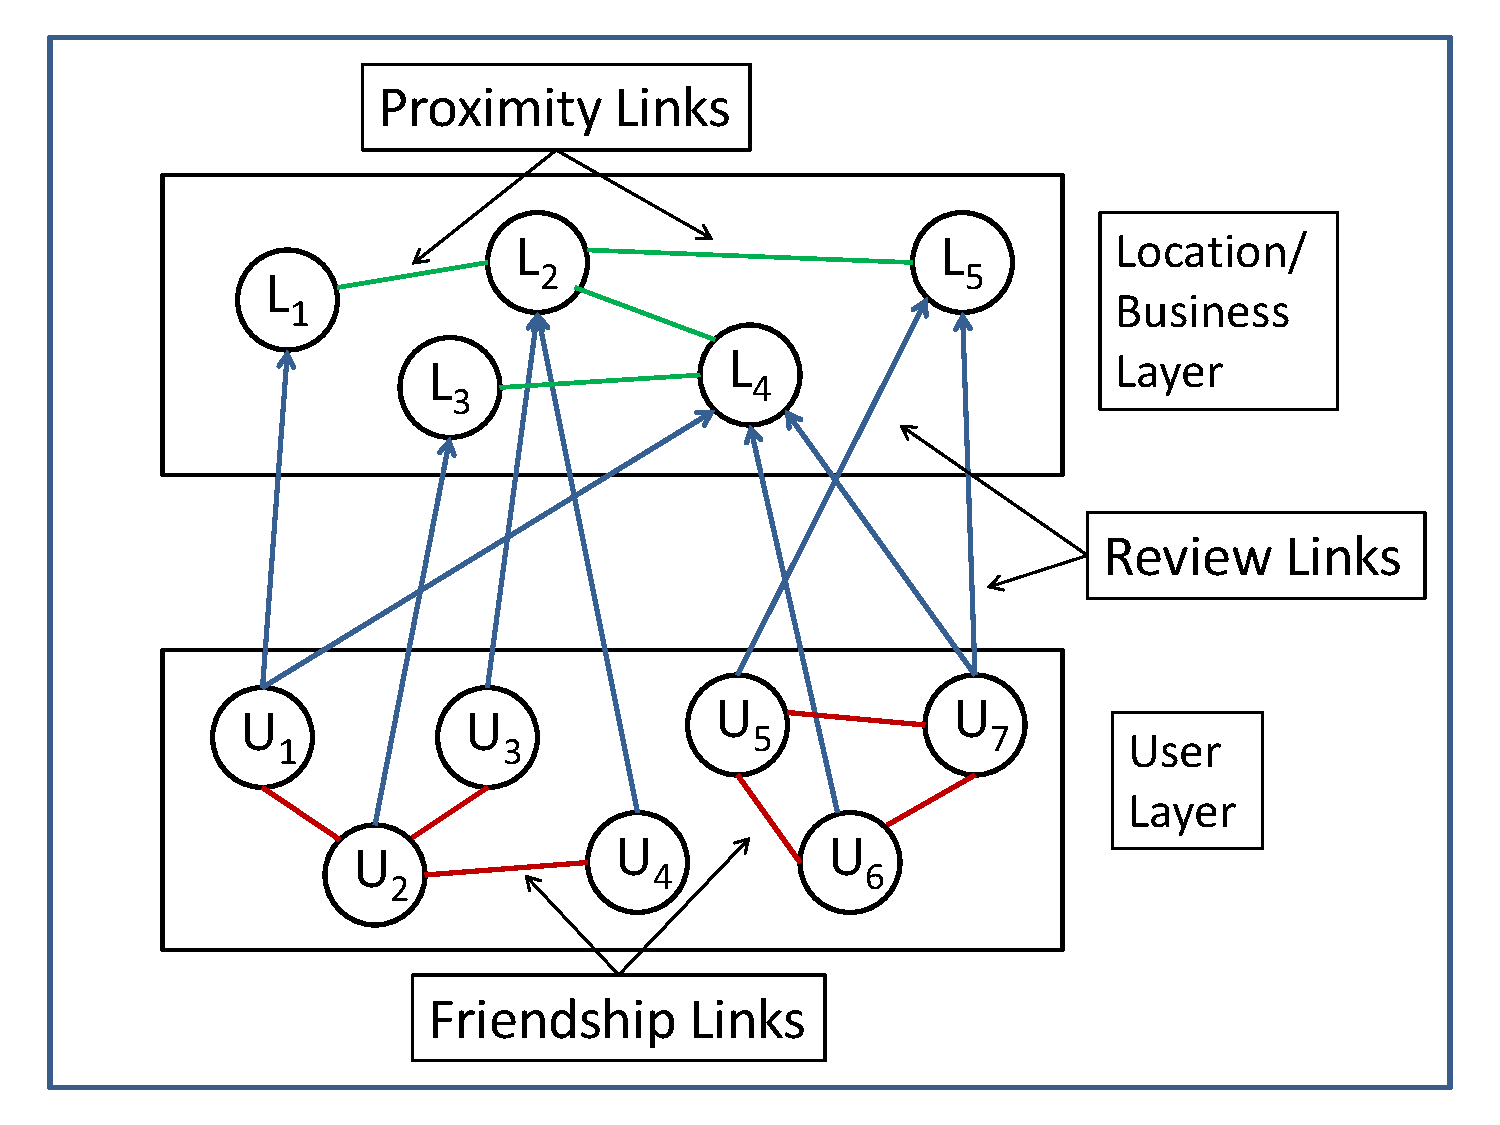
\includegraphics[width=2.3in]{./images/yelp_data.pdf}
\vspace{-0.1in}
\caption{A sample multilayer (Yelp) network.}
\vspace{-0.23in}
\label{yelp}
\end{figure}



% \begin{figure}
% \begin{center}
% \subfigure[A sample Yelp network
% ]{\label{nmi1}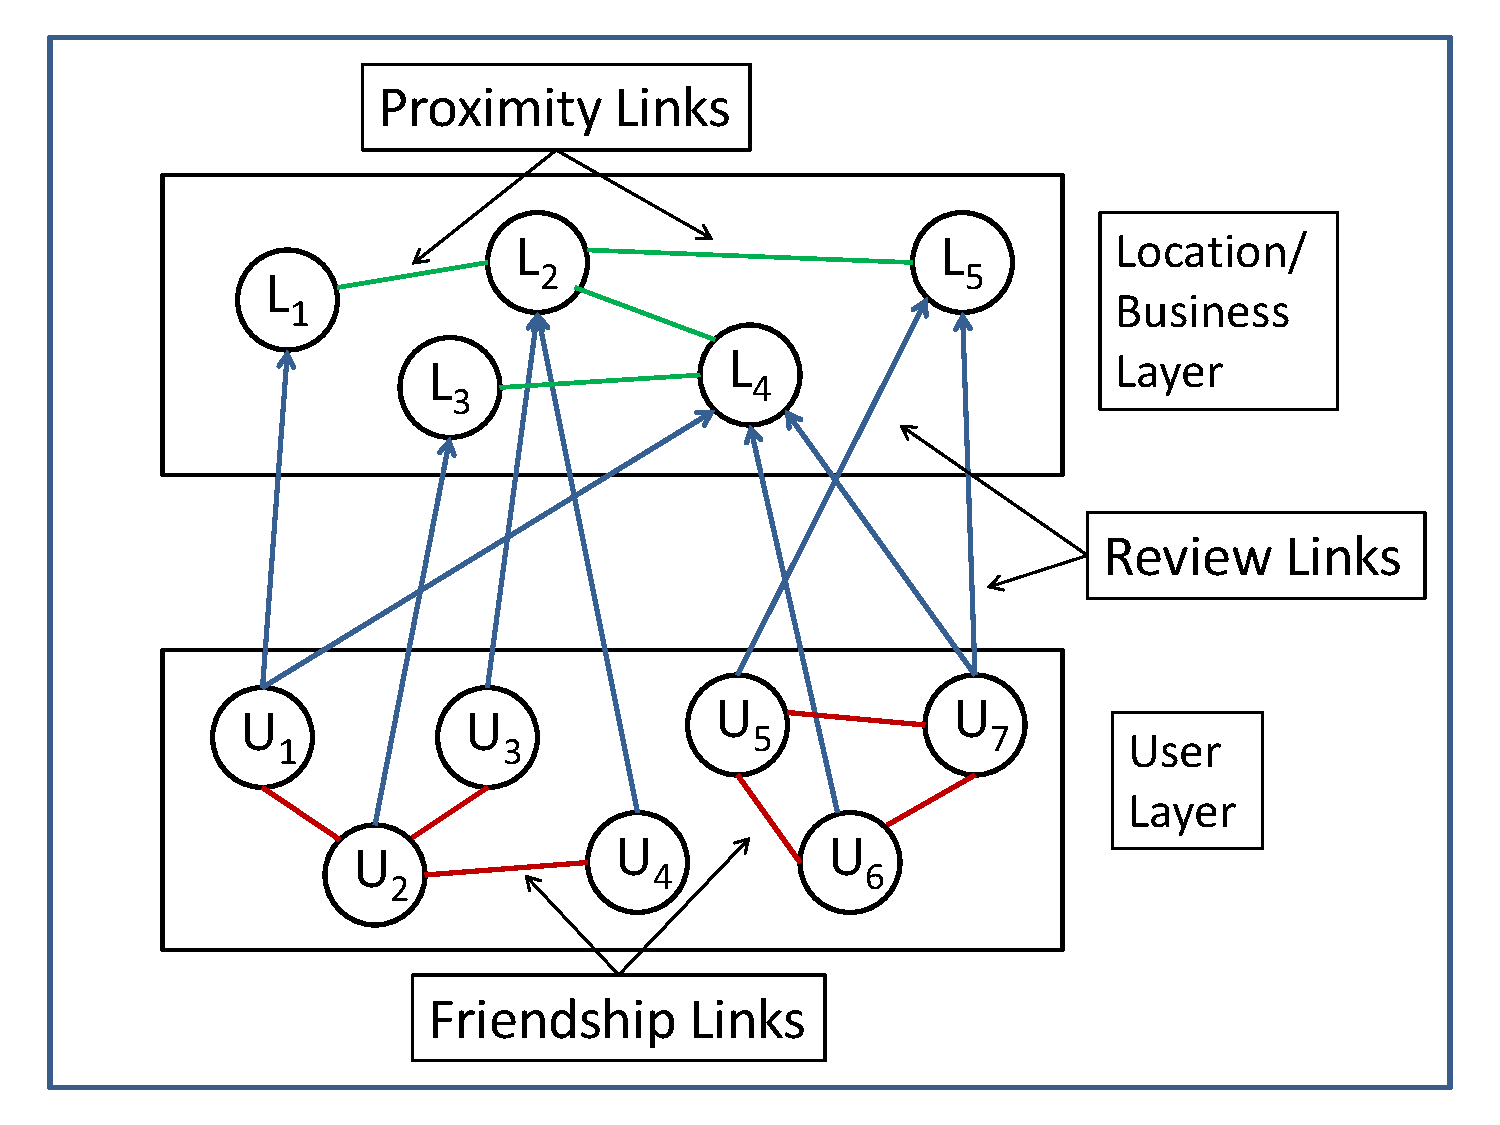
\includegraphics[angle=0,scale=.18]{./images/yelp_data.pdf}}
% \subfigure[A sample multilayer network with two different types of communities
% ]{\label{nmi1_1}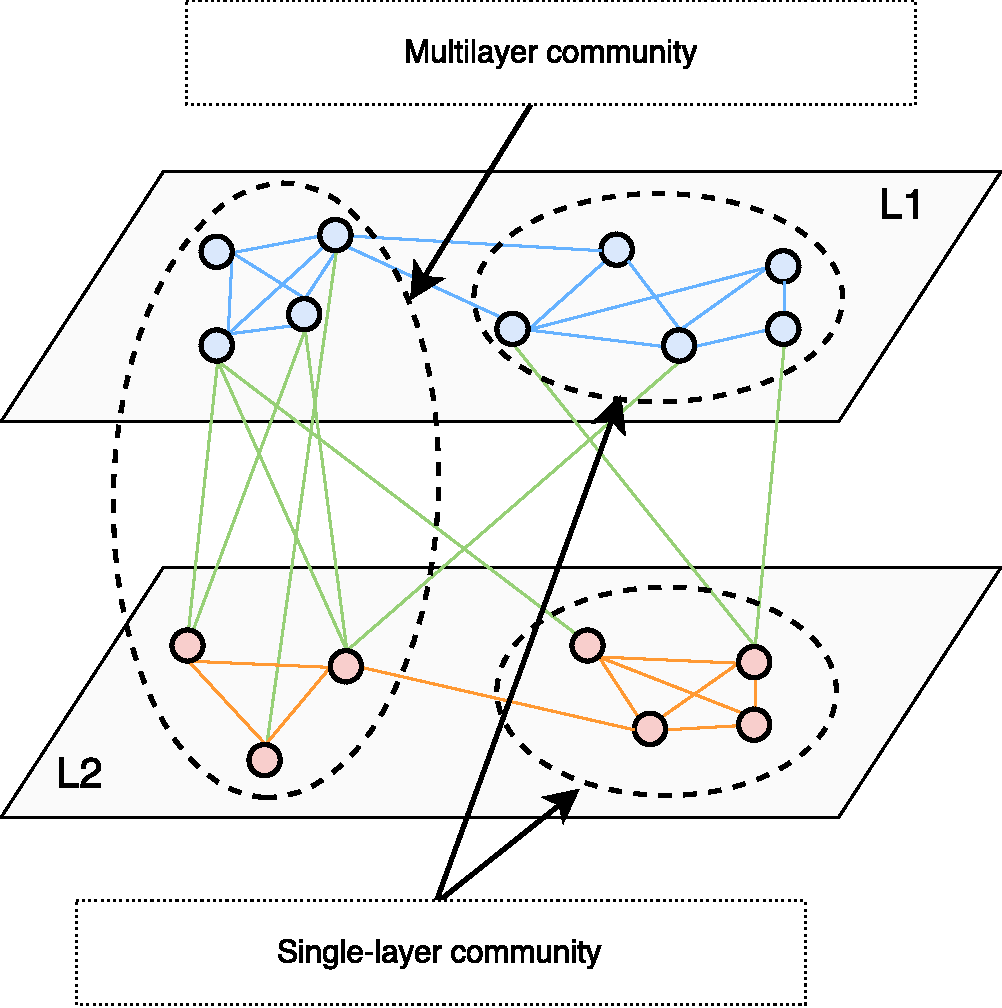
\includegraphics[angle=0,scale=.18]{./images/single_multi_community.pdf}}
% \end{center}
% \vspace{-0.1in}
% \caption{Sample multilayer networks}
% \vspace{-0.2in}
% \label{nmi00}
% \end{figure}



% \begin{figure*}
% \begin{center}
% \subfigure[A sample Yelp network
% ]{\label{yelp}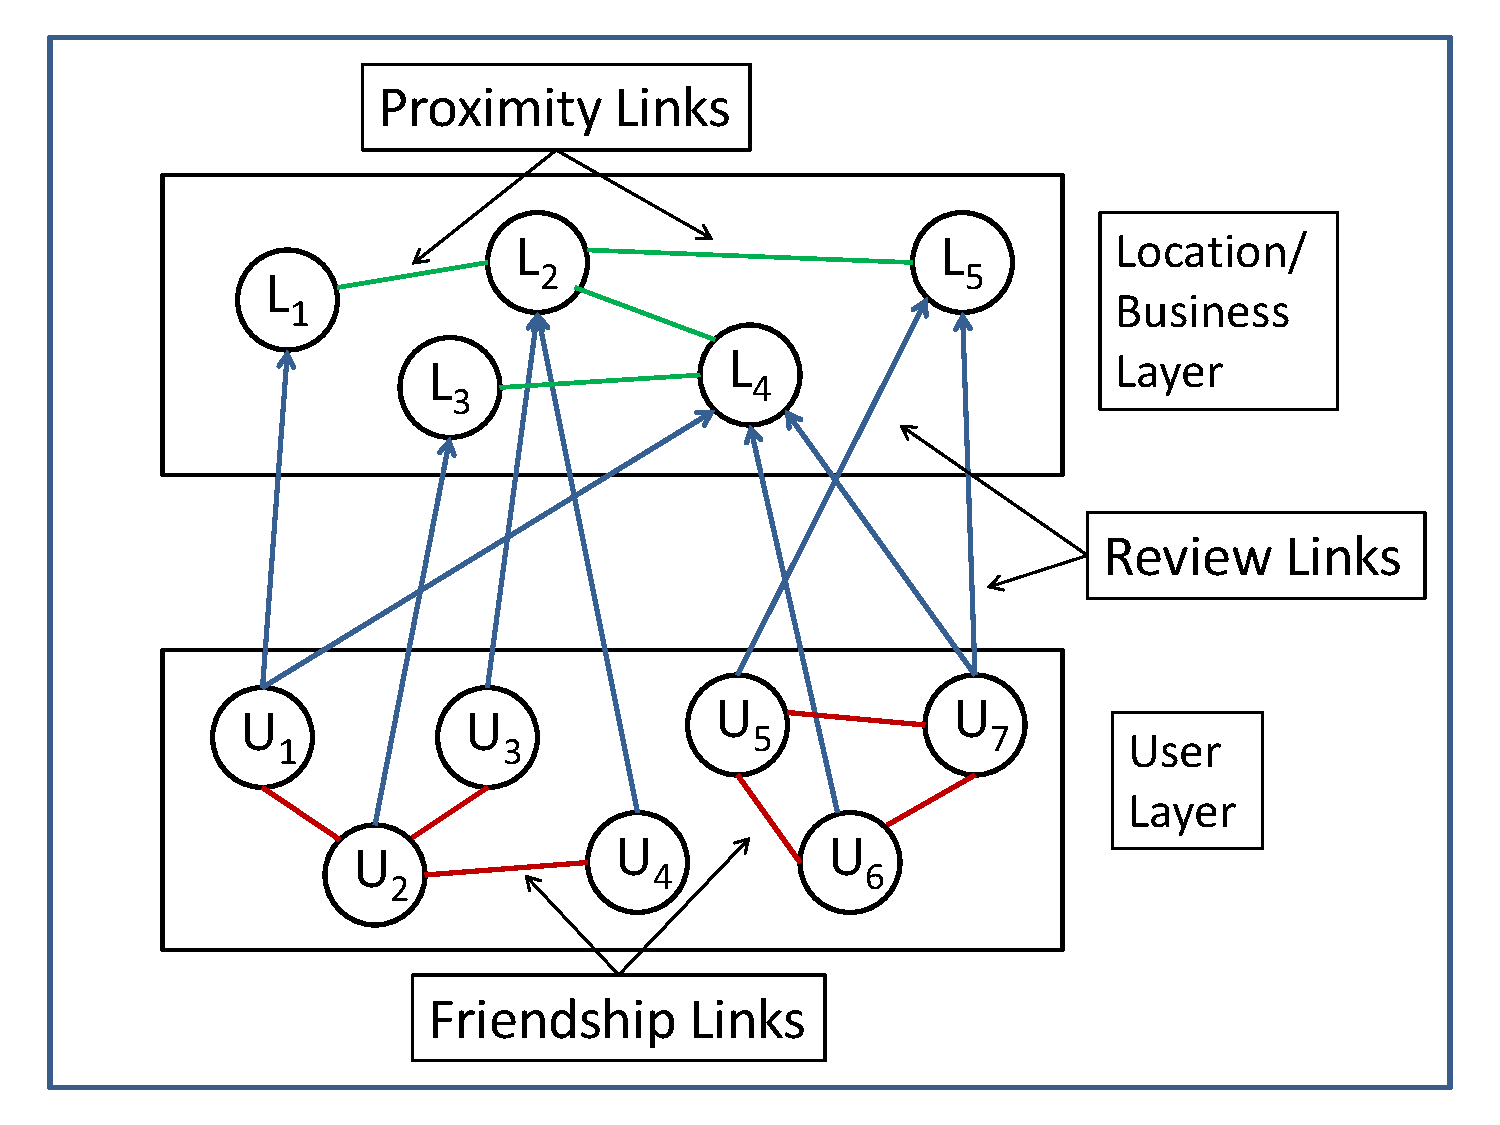
\includegraphics[angle=0,width=2.2in, height=1.5in]{./images/yelp_data.pdf}}
% \subfigure[Network configuration with two different ground truth communities
% ]{\label{N0}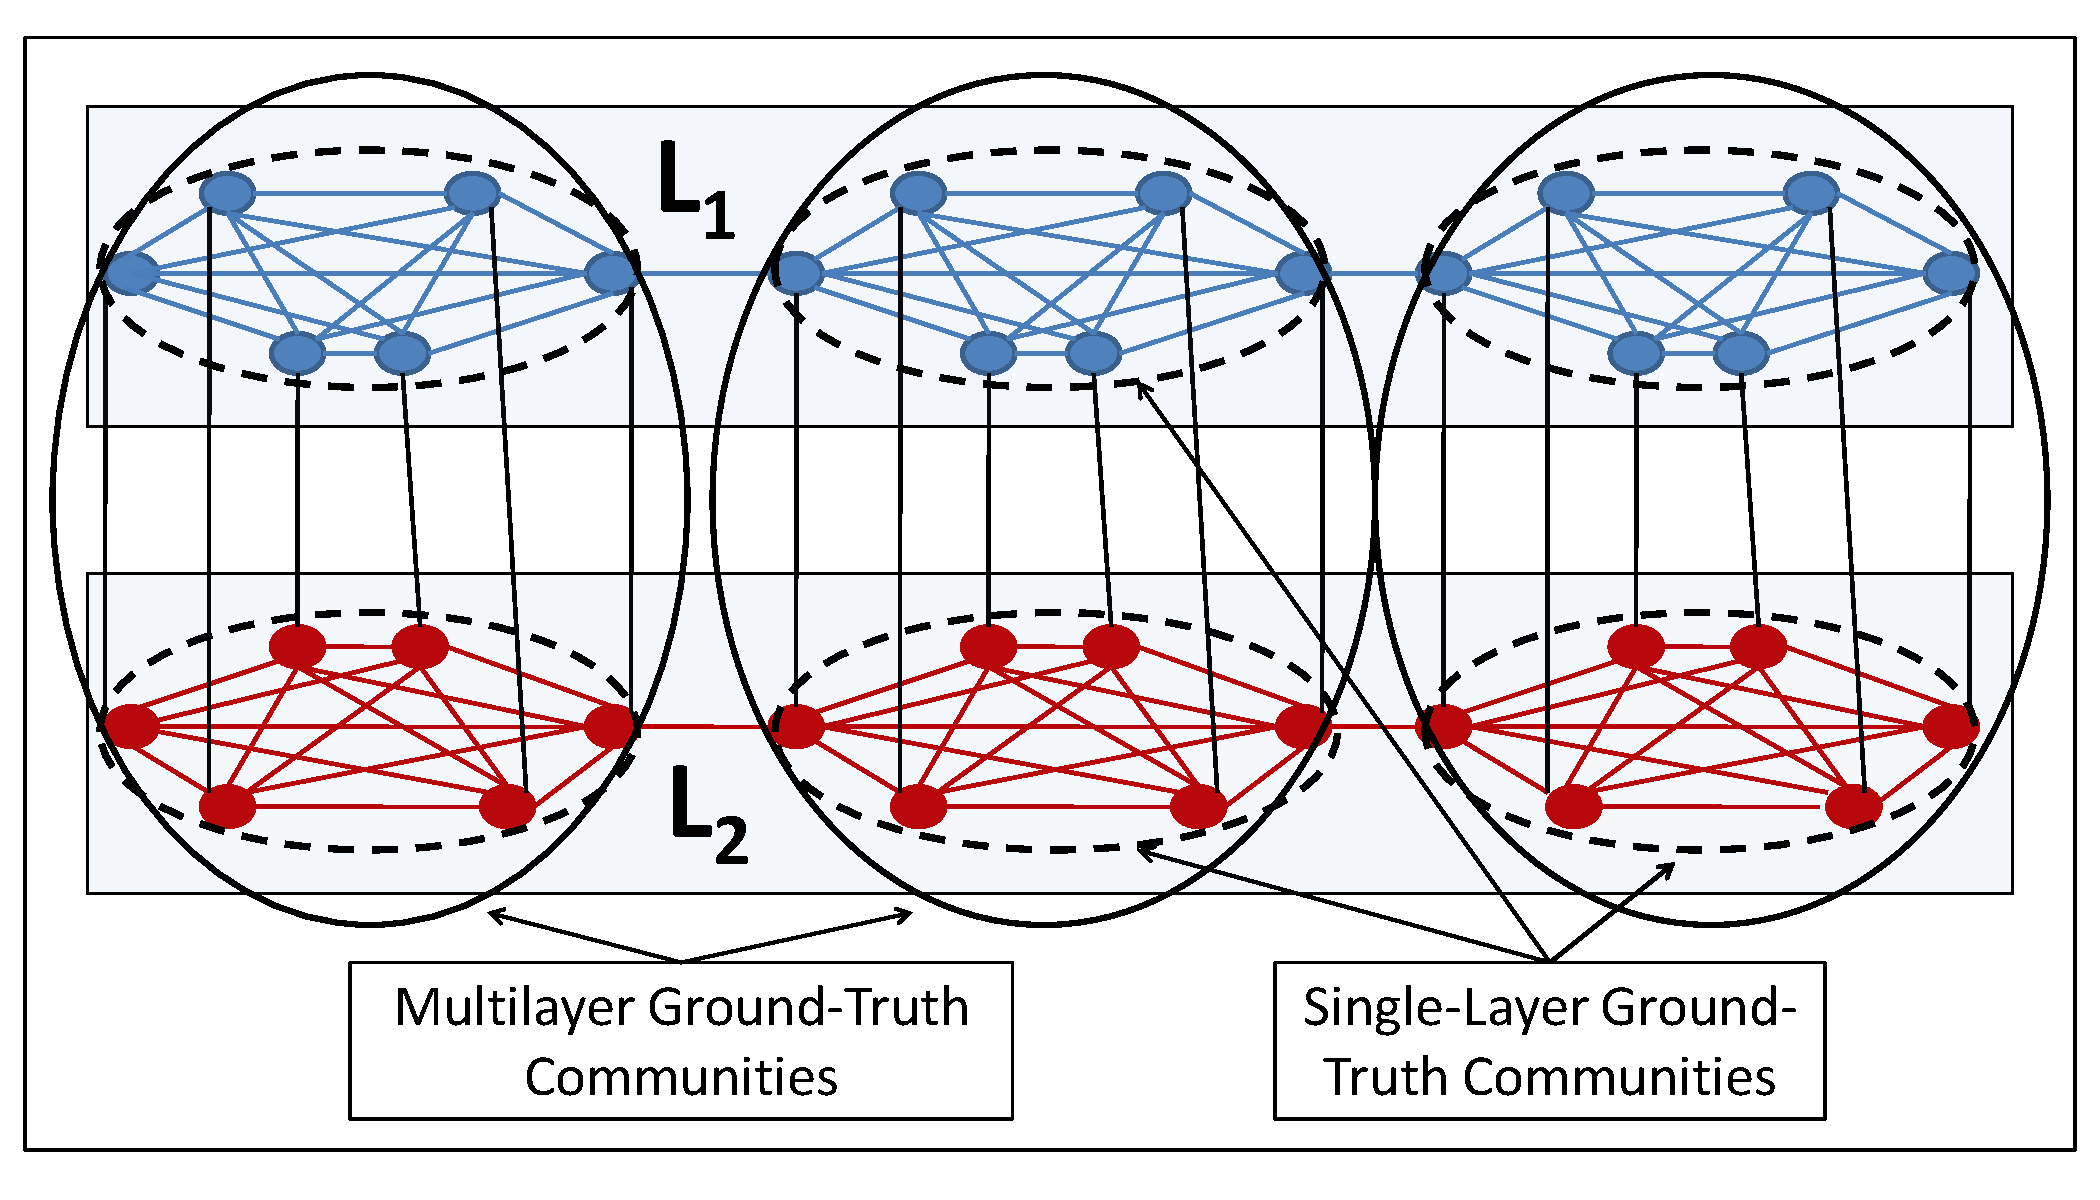
\includegraphics[angle=0,width=2.5in, height=1.5in]{./images/image31.pdf}}
% \end{center}
% \vspace{-0.25in}
% \caption{}
% \vspace{-0.2in}
% \label{YN0}
% \end{figure*}

% \begin{figure*}
% \centering
% 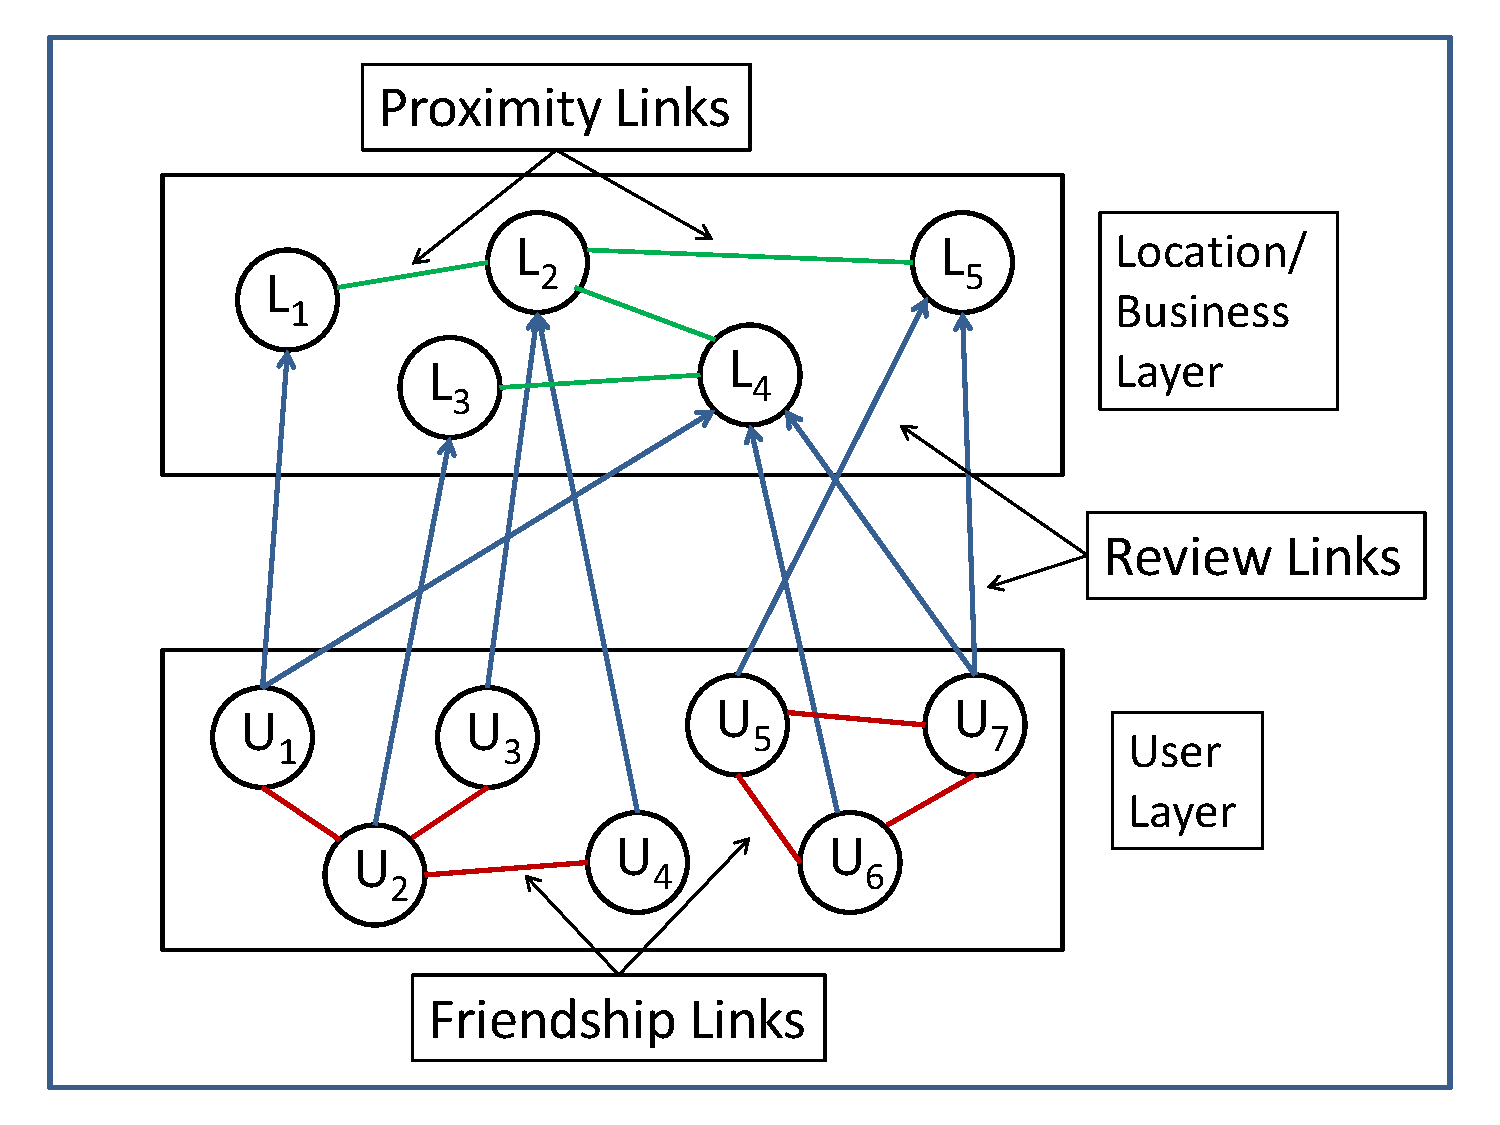
\includegraphics[width=2.5in]{./images/yelp_data.pdf}
% \vspace{-0.2in}
% \caption{A sample Yelp network}
% \vspace{-0.2in}
% \label{yelp}
% \end{figure*}

Community detection in complex multilayer networks is an important research problem.
%As we know, community detection i.e. the task of grouping objects based on their similarity, is one of the most important data mining tasks.
The communities in multilayer networks help to identify
functionally cohesive sub-units and reveal complex interactions between multi-type nodes
and heterogeneous links. They are also found to be beneficial for different
data mining tasks such as context-sensitive search, prediction and recommendation etc~\cite{metafac}. %[BM: need 1-2 good lines].
%provide an insight into how the system is internally organized~\cite{fortunato2010community,gulbahce2008art}. Such an analysis can also shed some light on the dynamics of group formation in the presence of heterogeneous interactions.
Community detection in multilayer network is challenging as the detected communities have possibility to contain only single or
multiple types of nodes.
Most of the recent endeavors concentrated on the
multiplex networks~\cite{mucha2010community,kuncheva2015community} where all layers share the
identical set of nodes but may have multiple types of interactions. In multiplex network, some of the approaches propose new quality
metrics~\cite{mucha2010community} to measure the goodness of the detected communities
%some approaches discover communities in each layer separately and then perform a frequent-pattern mining~\cite{berlingerio2013abacus}
whereas a few other
approaches utilize random walk~\cite{kuncheva2015community}
or frequent-pattern mining techniques~\cite{berlingerio2013abacus}
to obtain structurally similar components.
% There exists another school of
% research which discovers the communities in each layer separately and then perform a frequent-pattern mining~\cite{berlingerio2013abacus}.
In principle, most of the aforementioned algorithms transform the problem to the classical community detection in a monoplex network
leveraging on the fact that in multiplex network, one-to-one cross layer links connect the copies of the same nodes in multiple
layers. Unfortunately, the presence of heterogeneous nodes across multiple layers and cross layer dependency links make the
aforementioned solutions
inadequate for multilayer networks.
% Precisely, the communities detected in multiplex network possess only a single type of
% nodes which makes them difficult to extend for multilayer networks due to the presence of multiple types of nodes.

% collapse all the layers of the network into a single one and apply standard single layer community detection
% algorithms~\cite{rosvall2008maps,schuetz2008efficient,newman2004fast,duch2005community,clauset2004finding,newman2004finding,blondel2008fast} whereas.......
% [BM: need 1-2 lines summarizing the techniques of the multiplex comm detection]
%The naive approach is to collapse all the layers of the network into a single one and apply standard single layer community detection
%approaches~\cite{rosvall2008maps,schuetz2008efficient,newman2004fast,duch2005community,clauset2004finding,newman2004finding,blondel2008fast}.However, this approach suffer from massive information loss. [BM: one more line on the multiplex comm detection]



 %[BM: replace ineffective by a better word]

Attempts have been made in bits and pieces to detect communities in multilayer networks; novel methodologies have been
introduced such as Dirichlet % and non-negative matrix factorization~\cite{comar2012framework},
process~\cite{sun2014co}, tensor factorization~\cite{metafac}, subspace clustering~\cite{dong2014clustering},
non-negative matrix factorization~\cite{Cheng_kdd13} etc.
%and block model analysis~\cite{tang2012identifying} [BM: so many work? Want to reduce?].
% [BM: previous line is not clear.
% Need one good line to highlight the limitation. I write the following, but you try to add/revise.]
% However, most of these approaches suffer from several limitations.
% Some only work on a specific type of multilayer networks (say, star-type etc.)
% or are unable to detect communities comprising of multiple and single types of nodes simultaneously,
% others require to fix the number of communities apriori, limiting their capability to discover of the true set of communities.
% Finally, a proper framework to generate benchmark communities for generic multilayer network is not available for any of them.
However, most of these approaches suffer from several limitations. First of all, some of the aforesaid algorithms only work
on a specific type of multilayer networks (say, star-type~\cite{sun2014co} etc.). Secondly, some of them are
forced to detect communities comprising only multiple types of nodes~\cite{metafac}, hence introducing bias. Third, the desired number of
communities are required to be fixed apriori for most of them~\cite{metafac,dong2014clustering},
limiting their capability to discover the true set of communities.
Finally, a proper framework to generate benchmark communities for generic multilayer network is not available in any of them.

%
% Third, the desired number of communities are required to be fixed apriori for most of them,
% limiting their capability to discover of the true set of communities.
% Finally, a proper framework to generate benchmark communities for generic multilayer network is not available in any of them.

% Few attempts have been made in proposing modularity index for multilayer networks.
% Composite modularity~\cite{CompMod} calculates
% the modularity of a multi-relational network as the integration of modularities calculated for each single-relational subnetwork.
% However, due to the deficiency in definition,
% the composite modularity can only produce communities with single type of nodes. On the other side, modularity
% proposed in~\cite{medical_paper} in the context of gene-chemical interaction network fails to conceive the role of coupling links
% in community characterization.
% The detailed exploration of prior art reveals the importance of the multilayer community
% detection algorithm which is free from (a). any external parameter, say total number of communities (b). any bias towards
% communities with only single type or only multiple types of nodes.
% % The exploration of prior art reveals the importance to develop a proper modularity index that should tackle the limitations
% % discussed above.
% Developing a proper modularity index should be the first
% step towards this direction.

Recent endeavors directed towards development of modularity index for heterogeneous networks.
For instance, composite modularity~\cite{CompMod} calculates
the modularity of a multi-relational network as the integration of modularities calculated for each single-relational subnetwork.
However, due to the deficiency in definition,
the composite modularity can only produce communities with single type of nodes. On the other side, modularity
proposed in~\cite{medical_paper} in the context of gene-chemical interaction network fails to conceive the role of coupling links
in communities characterization. The detailed exploration of prior art reveals the importance of the multilayer community
detection algorithm which is free from (a) any external parameter, say total number of communities (b) any bias towards
communities with only single type or only multiple types of nodes. Developing a suitable modularity index should be the first
step towards this direction.

\begin{figure}
\centering
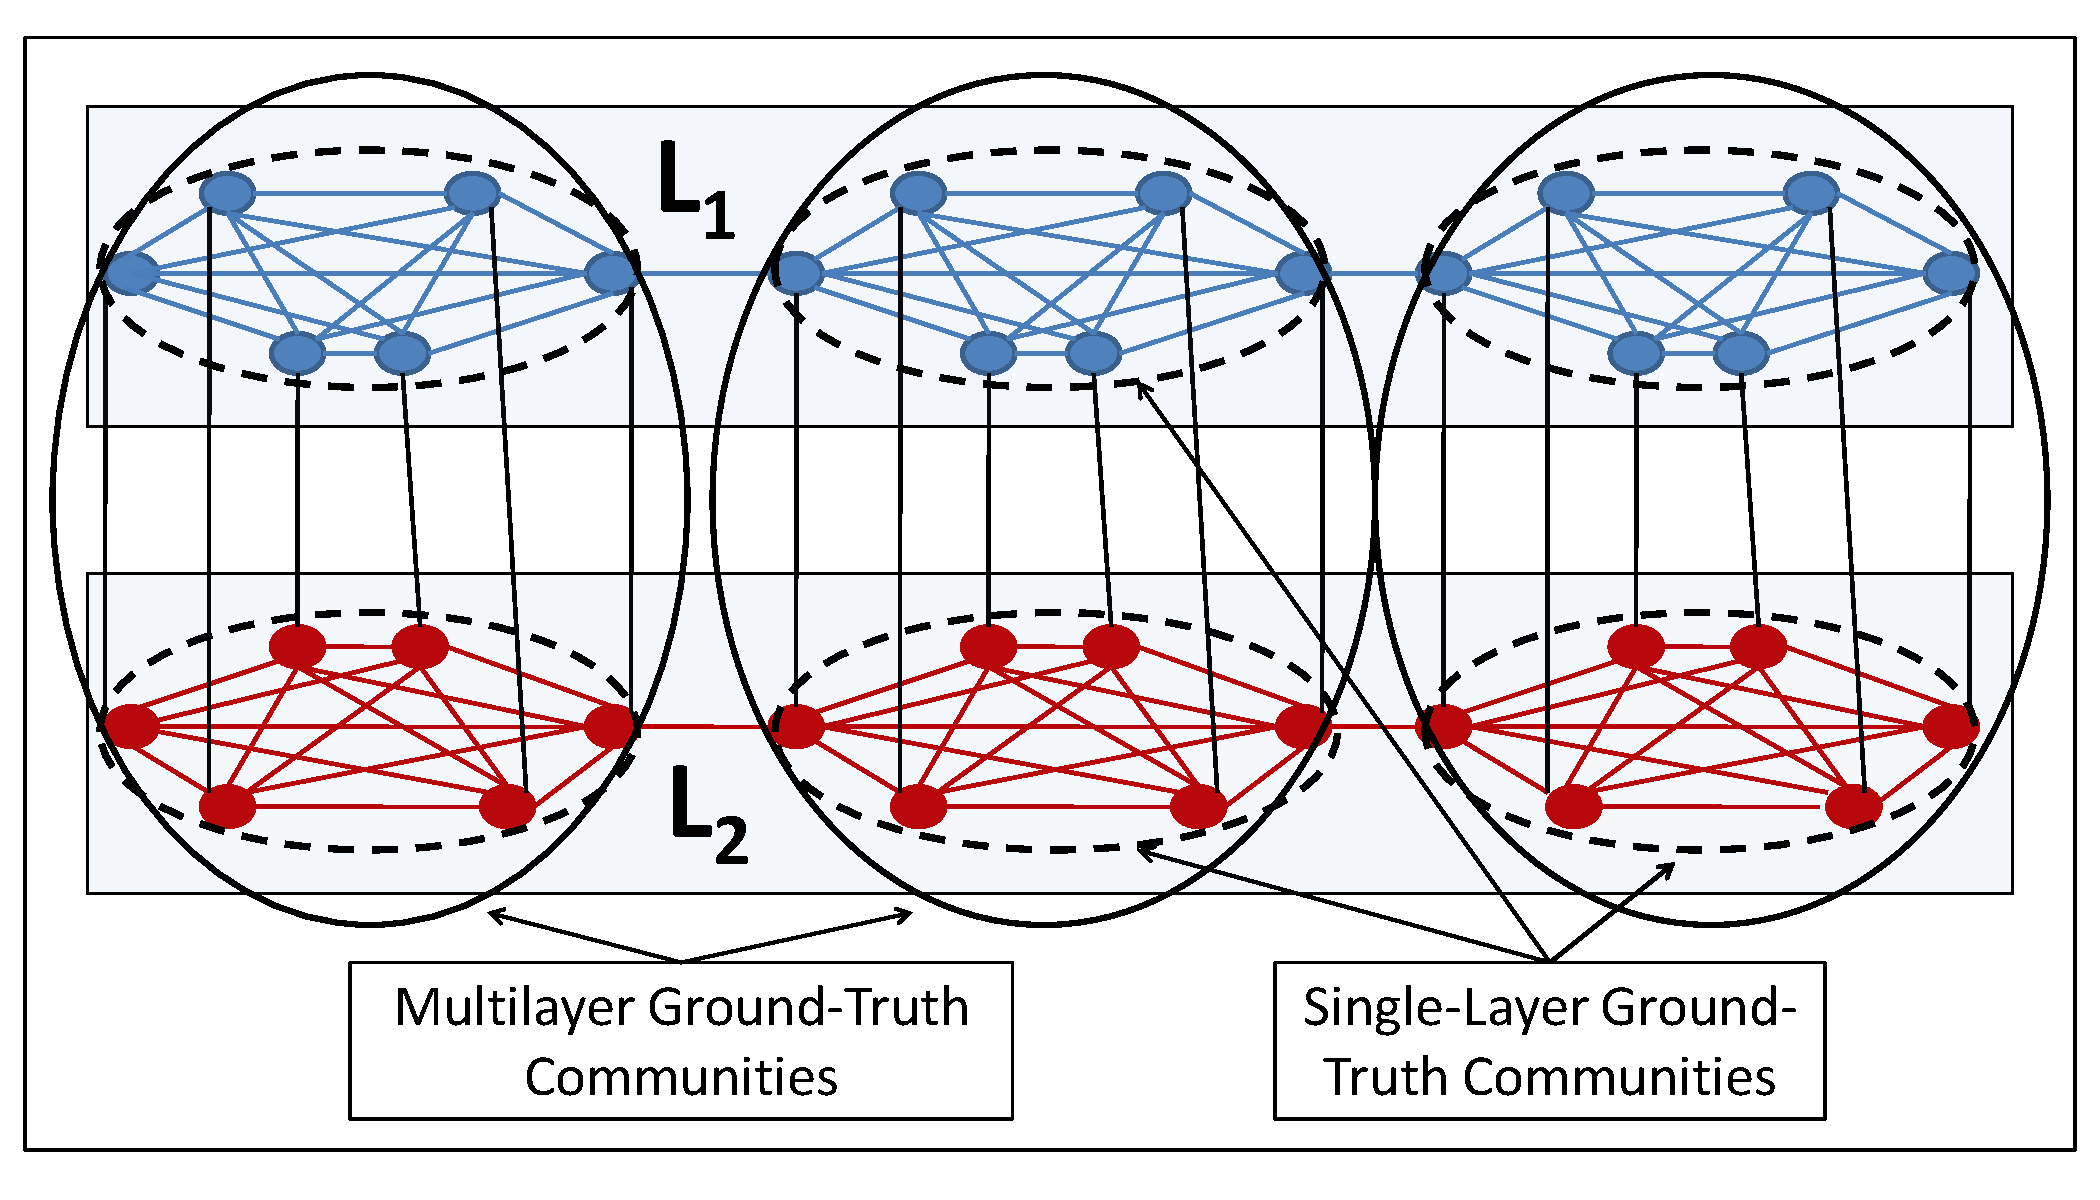
\includegraphics[width=2.3in]{./images/image31.pdf}
\vspace{-0.1in}
\caption{Network configurations with two different types of ground truth communities.}
\vspace{-0.23in}
\label{N0}
\end{figure}

\begin{figure*}
\begin{center}
% \subfigure[Avg source group-organizing group similarity of new members for successful \& unsuccessful groups
% ]{\label{T1}\includegraphics[angle=0,scale=.25]{./images2/fig3a.pdf}}
%\vspace{-0.12in}
\subfigure{\label{eval_01}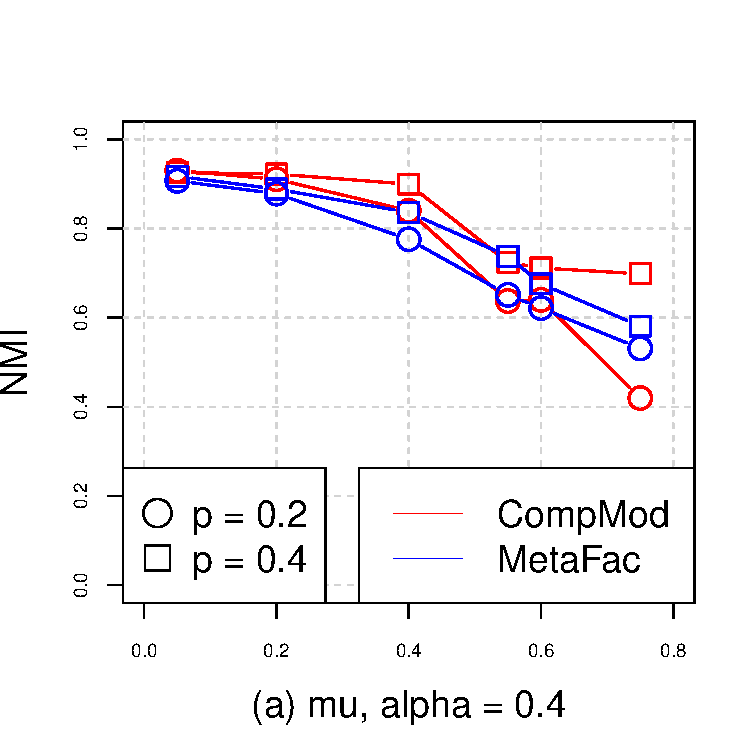
\includegraphics[angle=0,scale=.32]{./images/01.pdf}}
%\vspace{-0.12in}
\subfigure{\label{eval_02}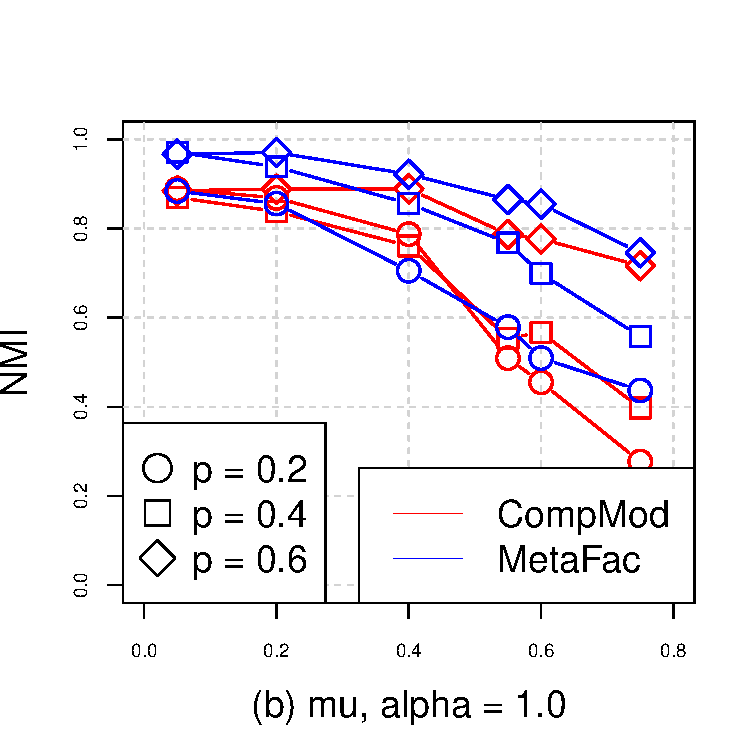
\includegraphics[angle=0,scale=.32]{./images/02.pdf}}
%\vspace{-0.12in}
 \subfigure{\label{eval_03}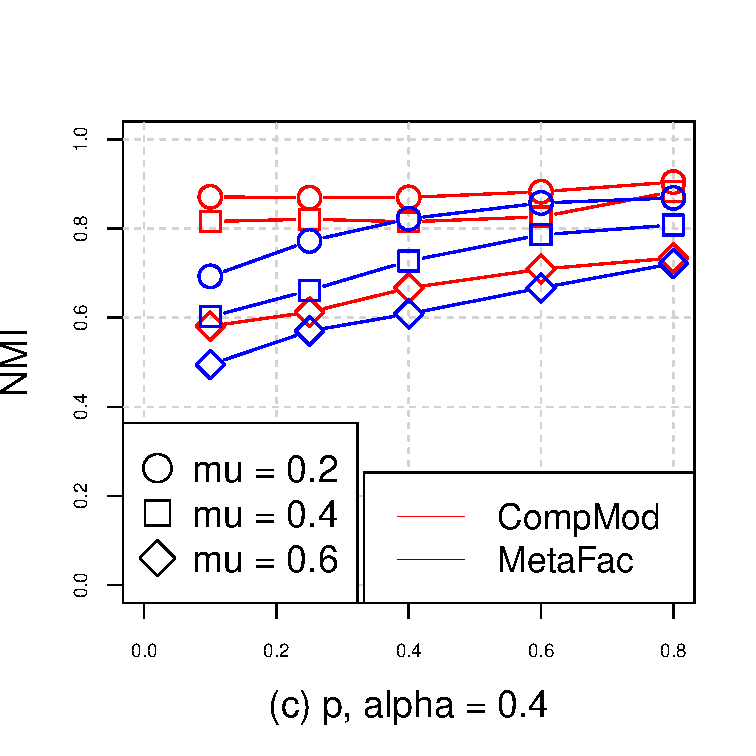
\includegraphics[angle=0,scale=.32]{./images/03.pdf}}
%\vspace{-0.12in}
\subfigure{\label{eval_04}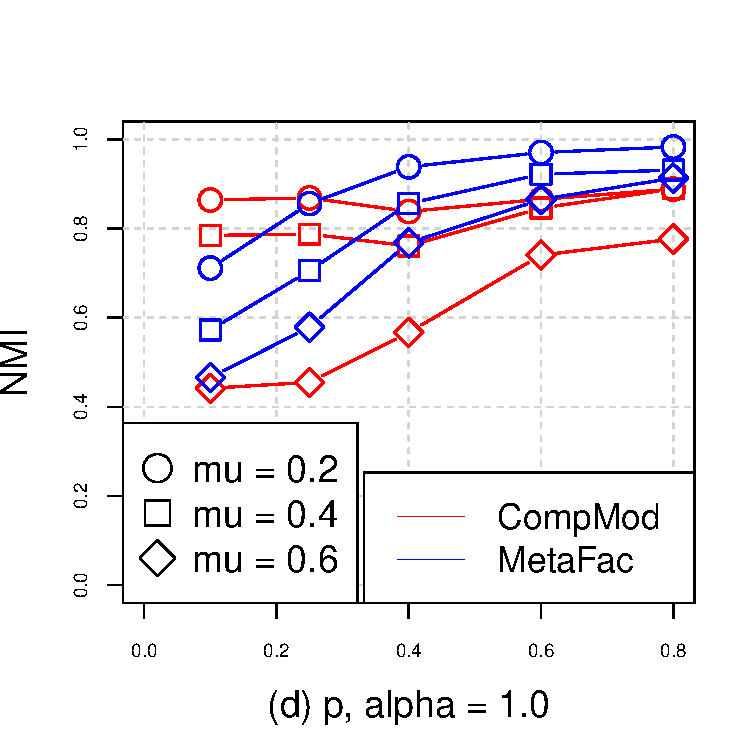
\includegraphics[angle=0,scale=.32]{./images/04.pdf}}

\end{center}\vspace{-0.22in}
\caption{Change of NMI values with $\mu$ and $p$ for `CompMod' and `MetaFac' on 2-layer networks with $100$ nodes in each layer,
generated with maximum degree $k^{i}_{max}=10$, average degree $\langle k_i\rangle=6$ \& coupling link density $d = 0.07$. }
\vspace{-0.22in}
\label{eval_syn}
\end{figure*}

% The idea is to decompose a
% multi-partite multi-relational network into multiple single-relational subnetworks, each composed of one type of edge
% and the incident nodes. Then, a composite modularity which is an integration
% of the modularity in each subnetwork is proposed for evaluating community
% structure in the multi-partite multi-relational network.
%Also, it cannot handle communities of many-to-many correspondence.

In this paper, we propose a community detection algorithm for multilayer networks
%as well as evaluate those communities with ground truth.
which is able to detect communities comprising both single type as well as multiple types of nodes,
depending on the network structure. First we represent the multilayer network with proper notations and define
the problem of community detection (sec.~\ref{dataset}). Next, we develop a methodology to construct synthetic multilayer network
with ground truth communities and evaluate it rigorously (sec.~\ref{syn_gen_eval}). The major contribution of this paper is to propose a
modularity index $Q_M$ for characterizing communities in multilayer networks. Subsequently, we develop the multilayer community detection
algorithms \textbf{GN-$Q_M$} and \textbf{Louvain-$Q_M$} incorporating the modularity index $Q_M$. We present the convergence proof for both 
the proposed algorithms along with their complexity analysis (sec.~\ref{metric}).
%[BM: one good line on we prove the convergence of \textbf{Louvain-$Q_M$} while fitting $Q_M$ into Louvain. May ask JL.]
We first evaluate the performance of the proposed modularity as a community scoring metric (sec.~\ref{ev_metric}) and then tested
the performance of the developed algorithms
against the competing algorithms.
Controlled experiments, performed on
the synthetic network, exhibit the ability of the \textbf{GN-$Q_M$} and \textbf{Louvain-$Q_M$} algorithms to
efficiently detect communities comprising both single types and multiple types on nodes (sec.~\ref{eval}). Finally,
we evaluate the proposed multilayer algorithms on the empirical dataset (Yelp and Meetup) and 
demonstrate that they outperform the state of the art baselines in correctly discovering the communities (sec.~\ref{emp}).
%[BM: one line on Meetup]
%[BM: add section numbers]
% \begin{enumerate}
%  \item Background
%  \item Existing approaches and limitations:\\
%  Most algorithms are for single layer and multiplex. Not suitable for generic multilayer. Very few works on multilayer networks
%  where nodes are different in different layers. These algorithms have the following limitations
%  \begin{enumerate}
%   \item No. of communities has to be told apriori for most of them.
%   \item Most of them either detect all single layer communities or all multilayer communities. Cannot balance optimally.
%   \item Some algorithms work only for a specific topology of multilayer networks - say, star type of networks etc.
%  \end{enumerate}
%
%  \item Scope: Proposing generic modularity and optimization technique; Proposing Benchmark synthetic multilayer networks for evaluation.
%  \item Contributions
% \end{enumerate}
%[BM: real network, recommendation?]

%The rest of the paper is organized as follows - in Sec.~\ref{dataset}, we describe the empirical and synthetic networks we use for
%evaluating our algorithm. Sec.~\ref{experiment} experimentally establishes the need of developing a new modularity
%index for multilayer networks. Sec.~\ref{metric} describes our proposed metric and community detection algorithm. In Sec.~\ref{eval},
%we evaluate our approach with respect to existing techniques and finally, in Sec.~\ref{conclus}, we conclude this paper along with
%future directions.

% %
% % There are studies on community detection in homogeneous multi-relational networks or multiplex networks (sometimes called
% % multi-dimensional networks~\cite{tang2012community}, or multi-slice networks~\cite{mucha2010community}). For example, researchers
% % developed methods for detecting communities in
% % a particular subclass of such networks, known as signed networks where each edge has a positive or negative
% % sign~\cite{traag2009community, yang2007community, bogdanov2010towards}.
% % Mucha et al. proposed a multiplex model for describing a homogeneous multi-relational network and developed a method based
% % on optimizing a generalized modularity known as stability~\cite{mucha2010community}.
% % In \cite{boden2012mining}, Boden et al. considers graphs with multiple edge types and edge attributes. In such graphs, densely
% % connected clusters are detected that also have similar attribute values.
% % Moreover, researchers proposed methods based on matrix
% % approximation~\cite{tang2012identifying}, seed-centric approach~\cite{hmimida2015community} and spectral analysis~\cite{tang2012community}.

\section{Representation \& Problem statement}
\label{dataset}
%\subsection{Representation \& Problem statement}
We start with formally representing the multilayer network and defining the respective communities. Next, we state the problem of 
detecting communities in multilayer network and the key challenges.
\subsection{Representation}
We represent a multilayer network as a
tuple $\mathcal{G} = (\mathcal{G_U},\mathcal{G_B})$ where $\mathcal{G_U} = \{L_i: i \in \{1, 2, \dots, M\} \}$ is a
family of $M$ uni-partite graphs (called layers of $\mathcal{G}$)
and $\mathcal{G_B} = \{L_{ij}: i,j \in \{1, 2, \dots, M\}, i \neq j \}$ is the family of bipartite graphs containing nodes from
individual layers and the cross layer interconnections among them.
We denote each layer $L_i=(V_i, E_i)$ where $V_i$ and $E_i$ are respectively the
set of nodes and intra-layer edges present in $L_i$. In the same line, we can represent $L_{ij}$ as a triplet $(V_i, V_j, E_{ij})$
where $\{E_{ij} \subseteq \{V_i \times V_j\}:~i, j \in \{1, 2, \dots, M \}, i \neq j\}$ is the set of coupling edges
between nodes of layers $L_i$ \& $L_j$.
% For each node $k \in V_i$, $d_k$ (intra-layer degree) denotes the number of other nodes
% it is connected to in the same layer and $c_k$ (inter-layer/coupling degree) denotes the number of other nodes it is connected
% to in the other layers via coupling edges.
% The elements of $\mathcal{E}$ (i.e. $E_{ij}$s) are called interlayer or crosslayer
% connections whereas the elements of each $E_i$ are called intralayer connections of layer $L_i$.



\textbf{Definition:} A community $C$ in a multilayer network $\mathcal{G}$ is defined as a cohesive 
module $(\mathcal{C_U},\mathcal{C_B})$ of $\mathcal{G}$
containing a subset of nodes from one or more layers and all the edges having both endpoints incident on them.
Mathematically, $\mathcal{C_U}$ and $\mathcal{C_B}$ can be
defined as
% where each $G^C_i$ is a subgraph of layer $G_i$ i.e. $G^C_i=$.
% On the other hand $\mathcal{C_B}$ is the subgraph of the bipartite graphs incident on the same set of nodes i.e.
$
\mathcal{C_U} = \{L^C_i = (V^C_i, E^C_i): V^C_i \subseteq V_i, E^C_i = \{E_i \cap (V^C_i \times V^C_i)\}, i \in \{1, 2, \dots, M\} \} ~and~
\mathcal{C_B} = \{L^C_{ij} = (V^C_i, V^C_j, E^C_{ij}): V^C_i \subseteq V_i, V^C_j \subseteq V_j, E^C_{ij} = \{E_{ij} \cap (V^C_i \times V^C_j)\}, i,j \in \{1, 2, \dots, M\}, i \neq j\}
$.

%It is evident that for any community $C$, it is not mandatory to contain nodes from each of the $M$ layers.
Importantly, communities of a multilayer network $\mathcal{G}$ can be divided into two
types (see Fig.~\ref{N0}) (a) cross layer communities (containing multiple types of nodes) 
for which $\left \vert \mathcal{C_B} \right \vert \neq \Phi$;
(b) single layer communities (containing only single type of nodes) for which $\left \vert \mathcal{C_B} \right \vert = \Phi$.


\subsection{Problem Statement}
The problem of multilayer community detection algorithm is to divide the network $\mathcal{G}$ into a set of disjoint cohesive
modules $C_1, C_2,\dots,C_K$ which is a cover of the nodes in $\mathcal{G}$ such that each module $C_i$ is comprised of a group of
nodes densely connected inside \& loosely connected outside the community.


% In such a setup, a community $C$ of $\mathcal{G}$ is defined as any subset of the set of nodes ($\{\bigcup_{i=1}^M V_i\}$)
% in $\mathcal{G}$, including all the edges incident on them. $C$ may contain nodes from only one layer or multiple layers. Accordingly, it is
% denoted as a single layer or multi layer community. Clearly, a single layer community contains only one type of edge whereas
% a multi-layer community can contain different types of edges.
% For example, if a multi layer community $C$ contains nodes from two layers $G_i$ and $G_j$, it can be conceived as a collection of
% three edge-based modules -
% i) module $1$ \& $2$ containing intra-layer edges from $E_i$ and $E_j$ respectively and ii) module $3$ containing cross layer edges
% from $E_{ij}$.
%In this work, our problem is to propose such a community detection algorithm which yields functionally cohesive communities
%from any given multilayer network.
% We also propose a modularity index which can measure the quality of the detected communities in terms
% of their intra-community and inter-community connection densities.

%\subsection{Challenges}
The key challenges of this problem are two-fold - (a) deals with multilayer network which contains multiple types of links (of different
densities) \& nodes and (b) detects both cross layer \& single layer communities simultaneously without any additional parameter.





% \begin{figure}
% \centering
% 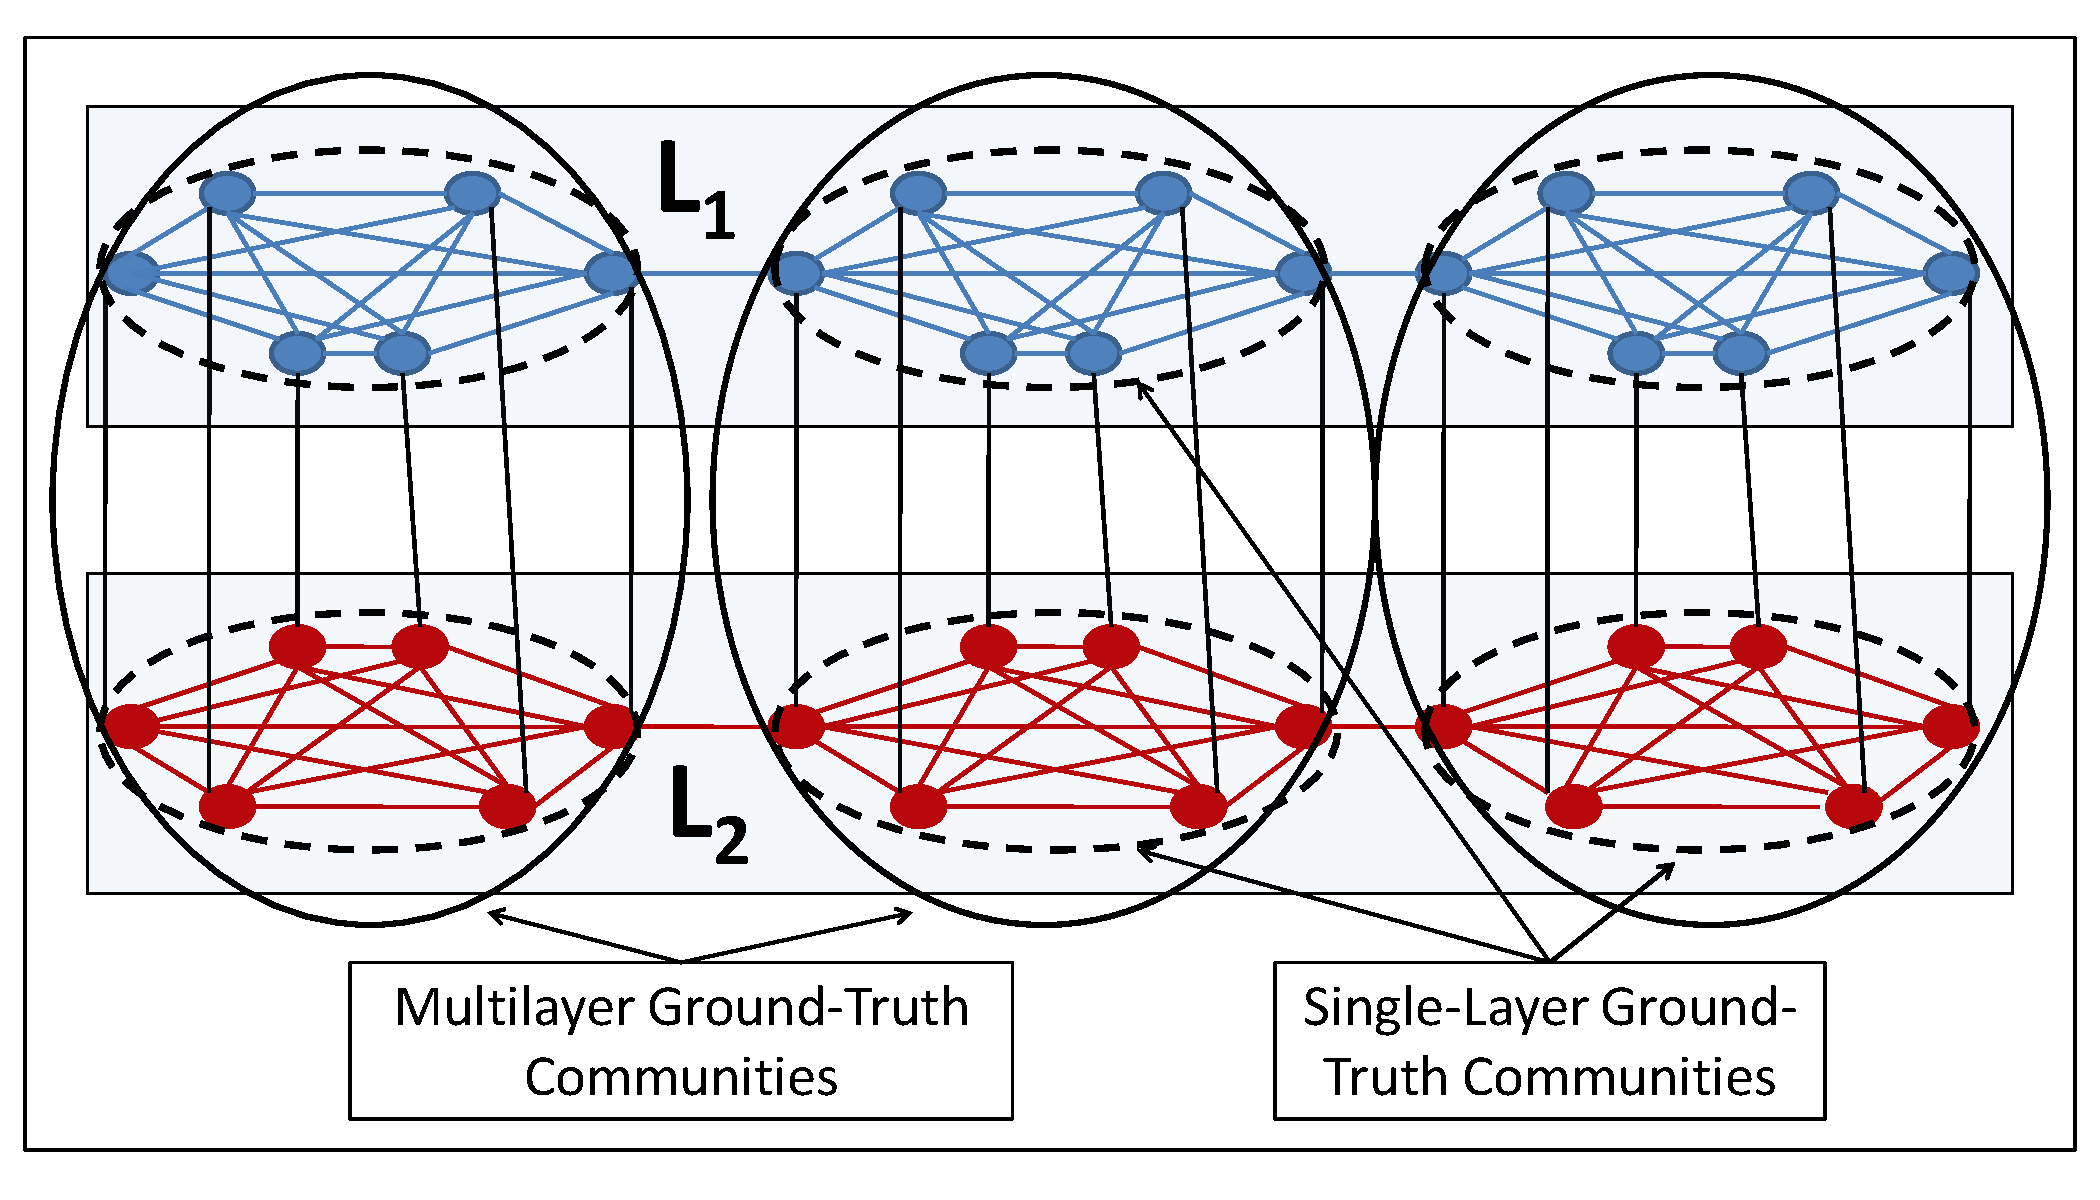
\includegraphics[width=2.5in]{./images/image31.pdf}
% \vspace{-0.1in}
% \caption{Network configuration with two different ground truth communities}
% \label{N0}
% \end{figure}
%
% \begin{figure}
% \centering
% 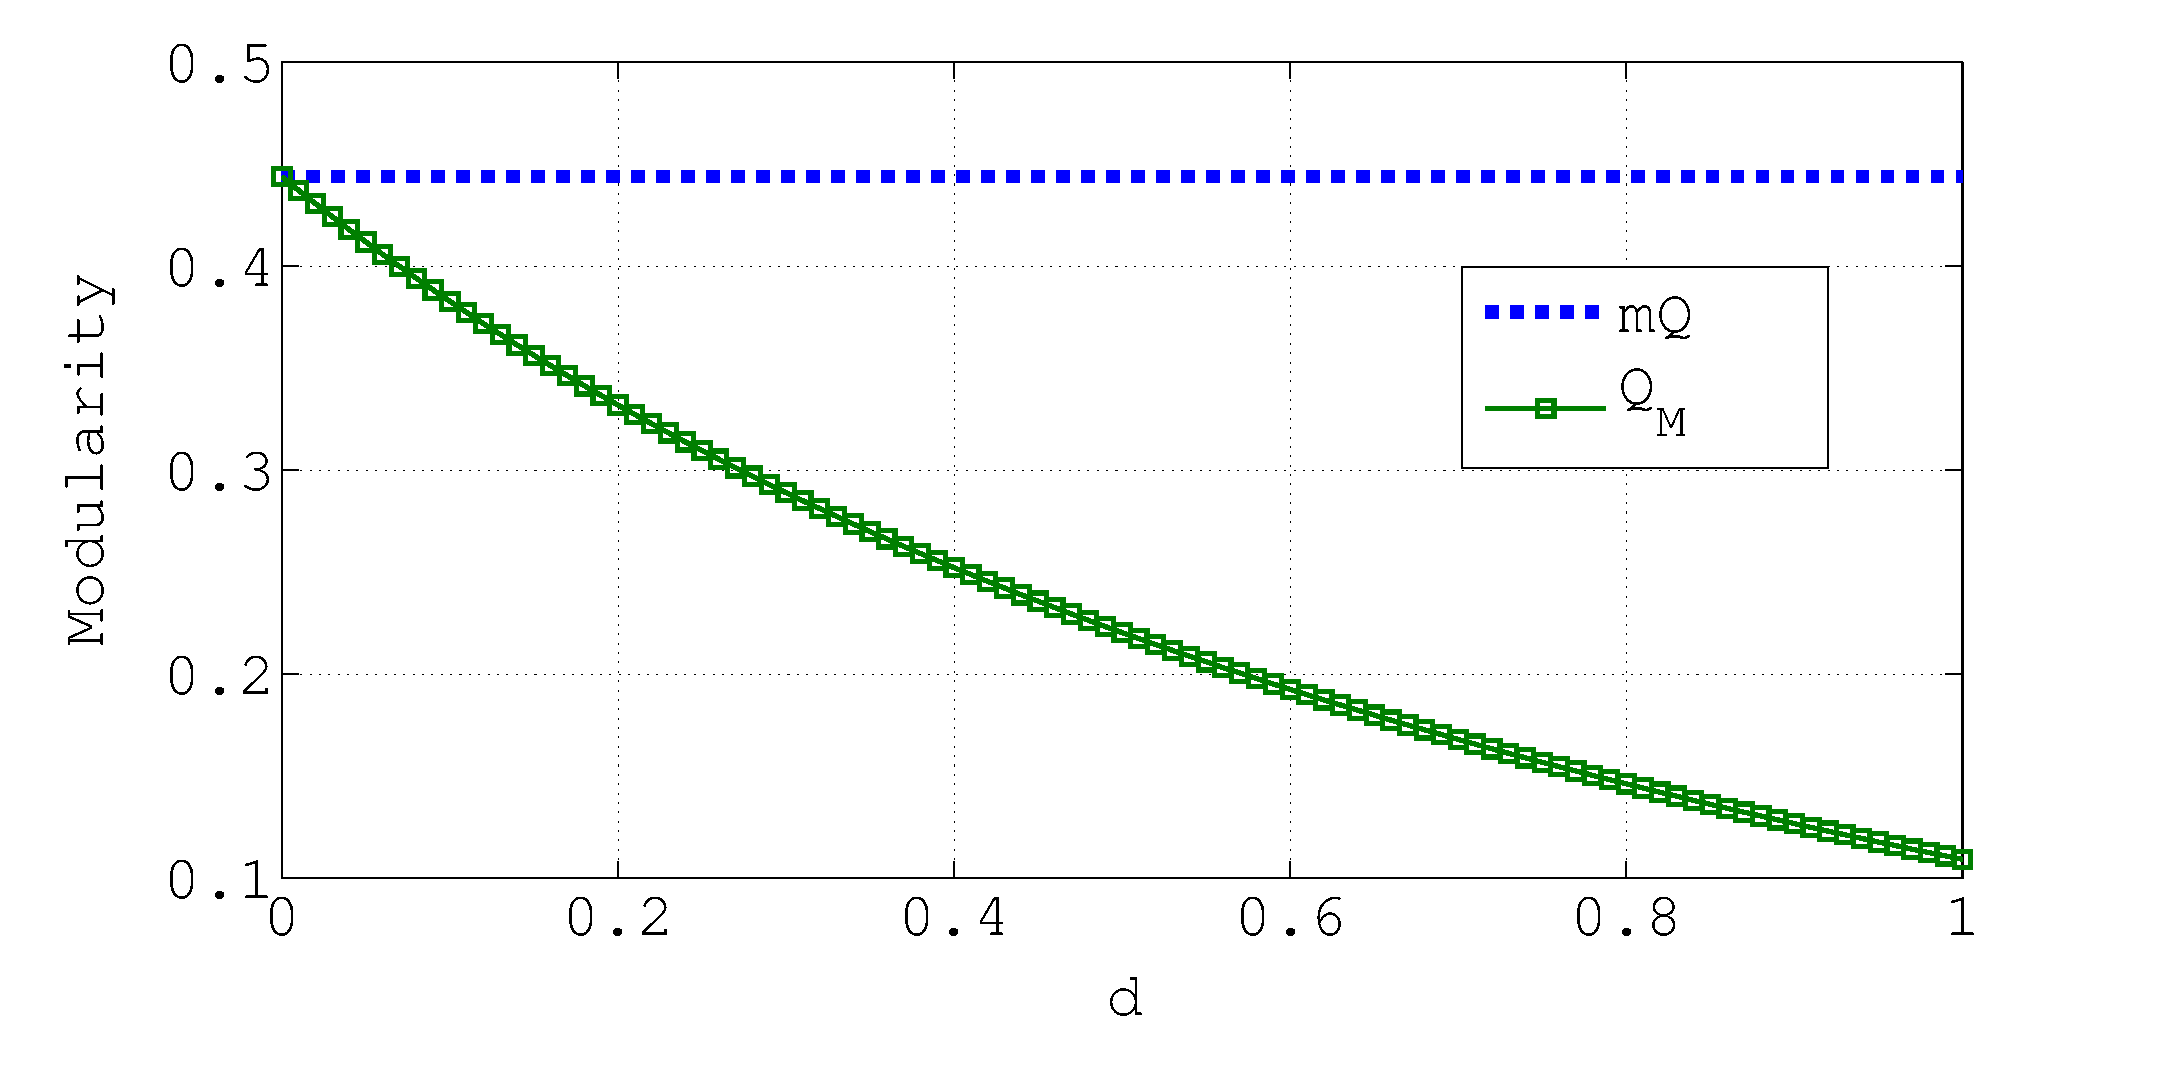
\includegraphics[width=2.5in]{./images/mQ_vs_march21_cross_single.pdf}
% \vspace{-0.1in}
% \caption{Comparison of $mQ$ and $Q_M$ for Config A while adding coupling links with different $P$ values}
% \label{cross_single}
% \end{figure}
%
% \begin{figure}
% \centering
% 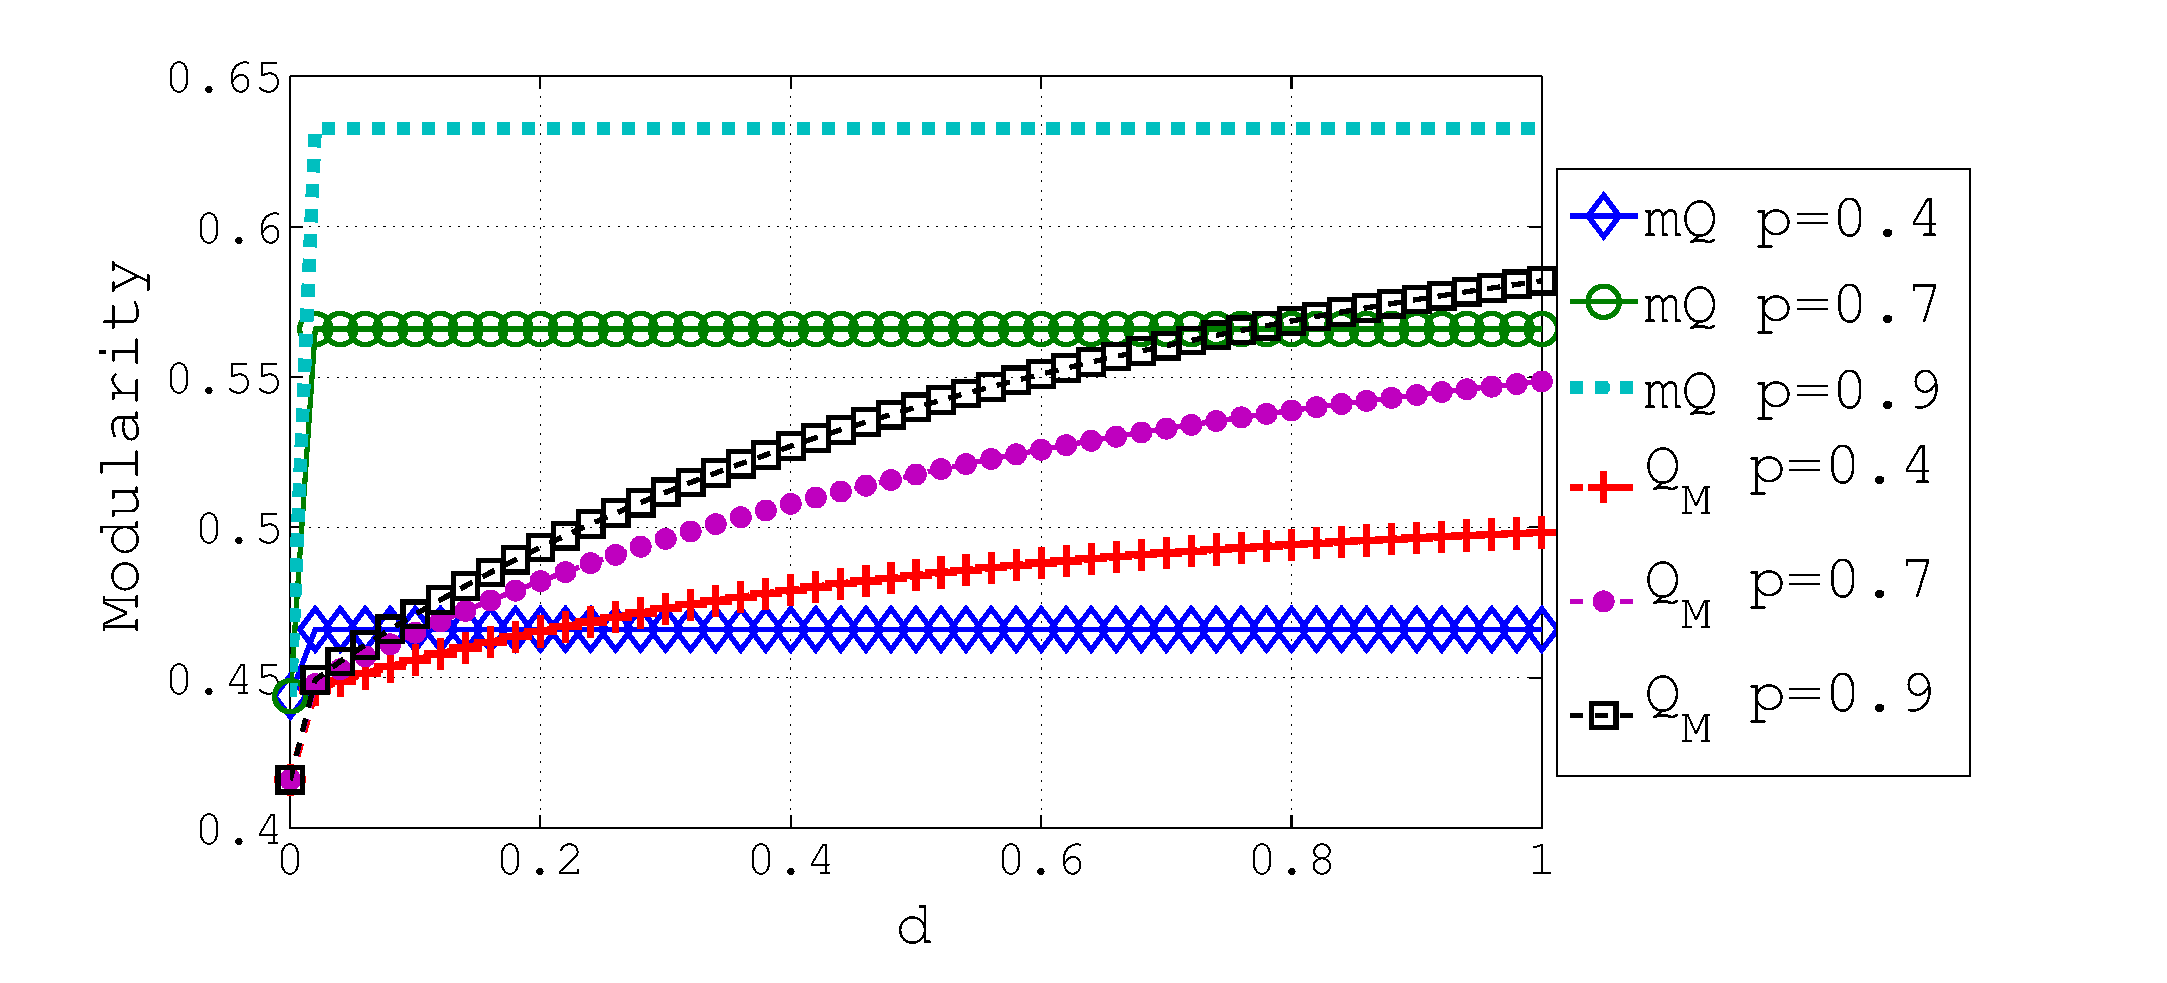
\includegraphics[width=3.5in]{./images/mQ_vs_march21_cross_multi.pdf}
% \vspace{-0.1in}
% \caption{Comparison of $mQ$ and $Q_M$ for Config B while adding coupling links with different $P$ values}
% \label{cross_multi}
% \end{figure}

\section{Dataset} \label{syn_gen_eval}
\subsection{Synthetic Dataset Generation}\label{syn_gen}
In this section, we propose a methodology to generate benchmark multilayer networks with ground truth communities.
% The ground truth communities can be of two types (a) cross layer communities (containing multiple types of
% nodes) (b) single layer communities (containing single type of nodes);
The parameter $\alpha$ regulates the
proportion of cross layer vs single layer communities in the benchmark. The network contains $M$ number of different layers where each
layer $L_i$ contains $N_i$ nodes ($N_i = \left\vert V_i \right\vert$) with average degree $\langle k_i\rangle$.
%The density of coupling links between the layers $L_i$ and $L_j$ is $d_{ij}$.
The methodology contains the following three steps:

\textbf{Step 1. Single layer communities:} First, we apply the LFR benchmark algorithm~\cite{lancichinetti2008benchmark}
to generate communities at
each layer $L_i$ with $N_i$ nodes where both degree and community size distributions follow power law distribution
with exponents $\gamma_i$ and $\beta_i$ respectively. We fix the mixing
parameter as $\mu_i$ to construct $\mathcal{C}_i$ single layer communities in layer $L_i$.

\textbf{Step 2. Cross layer communities:} We combine the community $x_i\in \mathcal{C}_i$ of layer $L_i$ with
community $x_j\in \mathcal{C}_j$ of layer $L_j$ to create the cross layer community $x_{ij}$. Assuming
$\left\vert \mathcal{C}_i \right\vert$ and $\left\vert \mathcal{C}_j \right\vert$ as the number of communities in
layers $L_i$ and $L_j$
respectively, $\left\vert\mathcal{C}_c\right\vert=min\{\left\vert\mathcal{C}_i\right\vert, \left\vert\mathcal{C}_j\right\vert\}$ denotes
the maximum possible number
of cross layer communities. We construct $(|\mathcal{C}_c| \times \alpha)$ cross layer communities by
randomly combining single-layer communities from both the layers $L_i$ \& $L_j$ respectively; notably each
cross layer community $x_{ij}$ may contain one or multiple single layer communities.

\textbf{Step 3. Coupling links:} Finally, we create the coupling links between the layers $L_i$ and $L_j$ with
density $d_{ij}$. Fraction $p$ denotes the mixing parameter for the cross layer communities. We first
distribute  $(N_i \times N_j \times d_{ij})$ coupling links randomly between the layers $L_i$ and $L_j$ where
each link has one end in $L_i$ and another end in $L_j$. Next, we rewire the coupling links such
that $p$ fraction of links stay inside the cross layer communities and the remaining $1-p$ fraction of
links connect different cross layer communities.

%[BM: Need to specify the typical parameters.]

\iffalse

suppose we have $|A|$ nodes in the top layer and $|B|$ nodes in the bottom layer,


For creating coupling links between every two layers,
 we utilise two parameters $d$ and $p$ where $d$ denotes the density of coupling links and $p$ denotes the fraction of such links
 within the mixed
 communities.

///////////////////////////////////////////
 \item Synthetic Dataset: Unlike single layer networks~\cite{lancichinetti2008benchmark}, there is no standard procedure to
 generate synthetic multilayer networks with
 ground truth communities. In ~\cite{Arenas}, the authors proposed such a method for multiplex networks. But it is non-trivial to extend
 it for generic multilayer networks. Hence, we propose a novel technique to generate multilayer networks with ground truth
 communities as described below.

 \begin{enumerate}

  \item \textit{Generating individual layers:} Suppose, we want to generate a network with $L$ layers. According to LFR
  benchmark~\cite{lancichinetti2008benchmark}, we
  generate $L$ subnetworks with ground truth communities. For generating each layer, we take standard LFR parameters such as
  number of nodes, average degree, maximum degree and mixing parameter ($\mu$), as input. The output network has $L$ isolated layers with
  each layer $A$ containing $n_A$ modules.

  \item \textit{Creating multilayer communities:} Once we get individual layers with ground truth communities, we group those
  communities across layers to create multilayer communities (containing nodes of different types).
  For example, suppose we have a 2-layer network where the top layer $A$
  has $n_A$ communities and bottom layer $B$ has $n_B$ communities. The maximum number of multilayer or mixed communities we can create
  is $n_c = min\{n_A , n_B\}$. We take another parameter $\alpha$ to decide the fraction of $n_c$ possible multilayer communities
  we actually create. Finally, we select $(n_C \times \alpha)$ communities from both $A$ and $B$ layers and randomly group
  them pair-wise so that each mixed community contains one single-layer community from both subnetworks $A$ \& $B$.

 \item \textit{Creating coupling links:} For creating coupling links between every two layers,
 we utilise two parameters $d$ and $p$ where $d$ denotes the density of coupling links and $p$ denotes the fraction of such links
 within the mixed
 communities. For the above example, suppose we have $|A|$ nodes in the top layer and $|B|$ nodes in the bottom layer,
 then we first assign
 $(|A| \times |B| \times d)$ crosslayer links randomly where each link has one end in $A$ and another end in $B$.
 After that, we rewire the links such that $p$ fraction of them stay inside the already created
 multilayer communities and the remaining
 $1-p$ fraction of them create cross multilayer-community links.

\end{enumerate}

 The parameter values chosen for generating networks for our experiments are mentioned in Sec.~\ref{eval}.
%  For our experiments, we use 2-layer synthetic networks where each layer is generated with identical LFR parameters. For each layer,
%  the total number of nodes is $100$, the average degree is $6$ and the maximum degree is $10$.
%  %and $\mu \in [0.05,0.40,0.75]$ (same across all layers for a particular network).
%  The other parameters i.e. $\mu$, $\alpha$, $d$ \& $p$ are varied from $0$ to $1$.
%

%  \textcolor{red}{[SP: Can we somehow generate crosslayer communities also with LFR? --- Raphael may check this part.
%  We should also check the multiplex LFR baseline available in website whether we can use it (possibly this is generated using the
%  method introduced in ~\cite{Arenas} ]).
%  }

 \item Real Dataset: Real multilayer datasets with ground truth communities are rarely available.
 So, we show the utility of our algorithm on real networks with the help of a recommendation task.
 First, we create a 2-layer network from an existing Yelp (a Location Based Social Network) academic dataset
 which is made available as part of the Yelp dataset challenge
 \footnote{\url{https://www.yelp.com/dataset\_challenge}}. Utilising that network, we obtain $K$ top recommended locations
 for each user with the help of collaborative filtering[REF]. Finally, in Sec.~\ref{eval}, we evaluate to what extent
 our detected communities can alleviate in such a recommendation task.

 The details of the dataset and the method to create the 2-layer network along with recommended locations, are described below.

 \begin{enumerate}
  \item \textit{Dataset Description:} The available Yelp dataset contains detailed information regarding visitors (Yelp users),
  business units (locations) and the tips (short business descriptions) \&
  reviews (detailed business description) posted by the visitors. Each business unit is indexed by
  a \textit{business ID}, and contains information about its category (restaurants, hotels, shopping etc.),
  latitude-longitude, address etc. as attributes.
  Similarly, each visitor is indexed by \textit{a user ID} and contains information regarding her city, social friendship connections etc.
  The dataset contains information of total $61184$ business units (comprising about $700$ different categories)
  located in $378$ cities and $366715$ visitors (with an average of $7$ social links) during the period $2005-2014$.
%   Each tip \& review entry is properly (daywise) timestamped and indexed by an unique \textit{tip/review id} containing the
%   corresponding visitor and business ID information.
  Additionally, there are nearly 1.6 million reviews and 0.5 million tips in the dataset.

  \item \textit{Creating 2-layer network:} We choose a particular city ``Las Vegas'' from the collection which contains
  $13601$ businesses and $173697$ Visitors visiting those locations. To reduce the size of the network, we first detect
  the maximally connected component in the friendship network of those $173697$ Visitors. This yields a set
  of $244$ connected users. Furthermore, we consider only the $1627$ locations which are at least reviewed once by anyone of them.
%   only the businesses
%   within 5 KM radius from the center of the city. This reduces the number of businesses to $1069$. Furthermore, we consider
%   only the $34563$ visitors who have written at least one review for one of those selected locations.
  After shortlisting the set of users \& locations, we create the layers of the
  network - the bottom layer consists of
  visitors who are connected with each other via friendship links and the top layer contains businesses
  where two businesses are connected
  if and only if they are within ZZ meters of each other.
  Finally, we add crosslayer (coupling) links between the nodes of this two layers with the help of
  reviews i.e. we connect a visitor with a business if she has written at least one review for that business (see Fig.~\ref{yelp}).

  \item \textit{Getting recommendations:} Collaborative filtering is a standard machine learning recommendation
  technique[REF]. Given the collection of visitor-business links,
  collaborative filtering (using business-business similarity) provides us with a set of $K$ top
  recommended (for future visit) businesses for each visitor.
%   Now, the visitors with more than a WW\% pair-wise similarity in their recommended set of
%   businesses are assumed to be liking similar locations and put in the same community. Thus, we create communities comprising of
%   similar minded visitors and the businesses they visited or prefer to visit.
%  [DETAILS]
 \end{enumerate}


\end{enumerate}
\fi


\subsection{Synthetic Dataset Evaluation}\label{syn_evalu}
In the following, we evaluate the performance of the synthetic network generation algorithm; we examine
%In order to verify that the generated networks are constructed properly i.e.
whether the generated networks behave consistently with our expectation. In order to accomplish the task,
we adhere to the following approach -
\textbf{(a)} we generate synthetic networks varying different model parameters $\mu$, $\alpha$ \& $p$, which intrinsically regulate the
quality of the community structures present in the generated networks.
\textbf{(b)} we apply state-of-the-art multilayer community detection algorithms~\cite{metafac, CompMod} on this synthetic networks
and evaluate the quality of the detected communities with respect to the ground truth communities.
\textbf{(c)} we conclude that the synthetic network possesses desired properties, only if the quality of the detected communities
in step (b) is consistent with the quality of ground truth communities specified in step (a).
% By doing so, we want to observe that parameters in usage have a real effect on the network structure and that they actually
% behave as expected.
% For instance, by tuning $\mu_i$ over its extreme ranges, it enables to control the fraction of internal and external edges of single layer communities in $L_i$.
% Comparably, $p$ parameter is used to control coupling links within and outside multilayer communities.

\subsubsection{Experimental Setup}
% For the experiments, we fix the number of nodes $N_i$ in each layer $L_i$ at $100$ with maximum degree $k^{i}_{max}=10$ \& average
% degree $\langle k_i\rangle=6$. The power-law exponents for degree distribution ($\gamma_i$) and community size distribution ($\beta_i$)
% for each layer are fixed at 2 and 1 respectively and the coupling link density $d$ is fixed at $0.07$.
% which has proved to be reliable [22].
% Then we adopt the normalized mutual information (NMI), a relevant measure of similarity of partitions that
% allows us to quantify the difference between a base partition, say $\La$, and another partition $P$ delivered by one of the algorithms.
We implement the following state-of-the-art multilayer community detection algorithms to detect the communities in step (b).
% In order to achieve this evaluation, we first implement the following two representative algorithms for community detection in
% multilayer networks.

(i) MetaFac~\cite{metafac}: This algorithm detects communities based on the tensor factorization and requires the number of
  communities to be specified apriori\footnote{For our experiment, we vary the input number of communities from two to fifty and report
  the one exhibiting highest overlap
 with the ground truth.}. It detects communities in a way such that each of them contains at least one node from every 
 layer (i.e. only cross layer communities). 
%  Therefore,
%  MetaFac algorithm
%  intrinsically assumes that nodes of different types can be grouped into same number of communities.
%   For our experiment, we vary the input number of communities from two to fifty and report the one exhibiting highest overlap
%   with the ground truth.

(ii) CompMod~\cite{CompMod}: This algorithm detects communities by maximizing \emph{composite modularity}, which is a
  combination of the modularities of different subnetworks.

We compute normalized mutual information (NMI)~\cite{danon2005comparing} index to compare the detected communities with the ground truth
communities (step (b)). $NMI$ is a measure of similarity of communities, which attains a high value if the ground truth and detected
communities
exhibit good agreement.



\subsubsection{Evaluation}
Finally, we accomplish the step (c) by demonstrating that synthetic network possesses the desired properties, in the following way.

\textbf{Varying $\mu$:} In Fig.~\ref{eval_01} and Fig.~\ref{eval_02}, we increase the mixing
parameter $\mu$ (fraction of edges going out of single layer communities) which degrades the qualities of the communities.
Clearly, as $\mu$ increases, NMI drops for both the state of the art algorithms, irrespective of $\alpha$ and $p$ values.
This points to the fact that with increasing $\mu$, the ground truth communities degrade independent of the type of communities,
which meets our expectation.
% Regarding single layer communities, assessments are ommitted in the present paper but can be found in~\cite{lancichinetti2008benchmark}.
% For datasets consisting of both single layer and multilayer communties, wide range of values for $\mu$ and $p$ have been
% selected to explore
% different graph structures.\bigvee
% Accordingly, the community structure is regulated by $\alpha$,
% single layer and multilayer communities together are obtained with $\alpha = 0.4$ and multilayer communities only with $\alpha = 1.0$.
%Thus we can denote two types of synthetic datasets, $D_1$ and $D_2$ respectively.
%Every curve show the variation of NMI either with $\mu$ or $p$.
% \\Fig~\ref{eval_01} and Fig~\ref{eval_02} focus on the mixing parameter $\mu$, for both value of $\alpha$.
% As the reader can notice, when $\mu$ increases NMI drops subsequently for any $p$ value.

\textbf{Varying $p$:}
Similarly, Fig.~\ref{eval_03} and Fig.~\ref{eval_04} focuses on $p$, which intuitively regulates the cohesiveness of
the cross layer communities. Evidently, the obtained NMI rises with $p$ for both the community detection algorithms. The slope is
observed to be relatively steeper for the higher $\alpha$, as it indicates the presence of
more number of cross layer communities (magnifying the effect of $p$).
% how $p$ parameter affects the network structures composed of multilayer communities.
% In comparison $mu$ is still playing a key role, especially when $p$ is low
% , that is to say when multilayer communities are less defined by coupling links but more by intra-layer edges.
% Reasonably, $p$ parameter has little effect on decreasing the structure of single and multilayer communities (see~Fig\ref{eval_01}
% and Fig\ref{eval_03}).
% This is expected because most of communties are single layer ($60\%$) and thus coupling links are less significant.
% This is also expected and reinforce our confidence on this synthetic dataset generation.

%Hence, for both the parameters $\mu$ and $p$, the generated synthetic networks behave exactly the way they are expected to, confirming the robustness \& reliability of our proposed synthetic network generation mechanism. 
%\section{Motivational Experiments}
\label{experiment}


In literature, we find only two modularity definitions for multlayer networks - one by Liu et al. in~\cite{CompMod} and the other 
by Song et al. in~\cite{medical_paper}. We have already discussed the limitations of the definition proposed in~\cite{CompMod}
in Sec.~\ref{intro}.
In this section, we criticize the metric proposed in~\cite{medical_paper} with the help of different synthetic network
configurations and emphasize on the need of proposing a new modularity metric for generic multilayer networks.

% As we mentioned before, some of the existing methods only find multilayer communities and some of them only find single layer communities.
% The algorithm proposed in \cite{medical_paper} seems to be our closest competitor at present. So, in the following we criticize the modularity
% metric they proposed.
For a 2-layer (suppose, A and B) network $G=G_A \cup G_\pi \cup G_B$ where $G_A$ = ($V_A$, $E_{AA}$) is the subnetwork 
of class A, $G_B$ =
($V_B$, $E_{BB}$) is the subnetwork of class B, and $G_\pi$ = ($V_A$, $V_B$, $E_{AB}$) is a bipartite graph connecting
nodes of class A and class B, the modularity metric proposed in \cite{medical_paper} is defined as 
\begin{equation}\label{eqn1}
 mQ=\frac{1}{3}\sum_{c=1}^{n_c}\{[\frac{I_{Ac}}{m_A}-(\frac{d_{Ac}}{2m_A})^2]+[\frac{I_{\pi c}}{m_\pi}-\frac{k_{\pi c}\times{d_{\pi c}}}{{m_\pi}^2}]+
 [\frac{I_{Bc}}{m_B}-(\frac{d_{Bc}}{2m_B})^2]\}
\end{equation}
where $n_c$ is the number of modules in a given partition; each module c is virtually divided into three
submodules, c = $(Ac)\cup(\pi c)\cup(Bc)$, $Ac$ is the submodule with links from $E_{AA}$, $\pi c$ is from $E_{AB}$
and $Bc$ is from $E_{BB}$; $I_{Ac}$ is the number of links in submodule $Ac$, $m_A$ is the size of subnetwork
$G_A$, $d_{Ac}$ is the sum of degrees of all $Ac$ nodes in $G_A$; $k_{\pi c}$ is the sum of degrees of A nodes of $\pi c$
in subnetwork $G_\pi$, $d_{\pi c}$ is the sum of degrees of B nodes of $\pi c$ in $G_\pi$.
In fact, this definition is basically a linear combination of Newman-Girvan modularity for simple graph~\cite{newman2004finding} 
and Barber modularity for bipartite graph~\cite{barber2007modularity}.

\begin{figure}
\centering
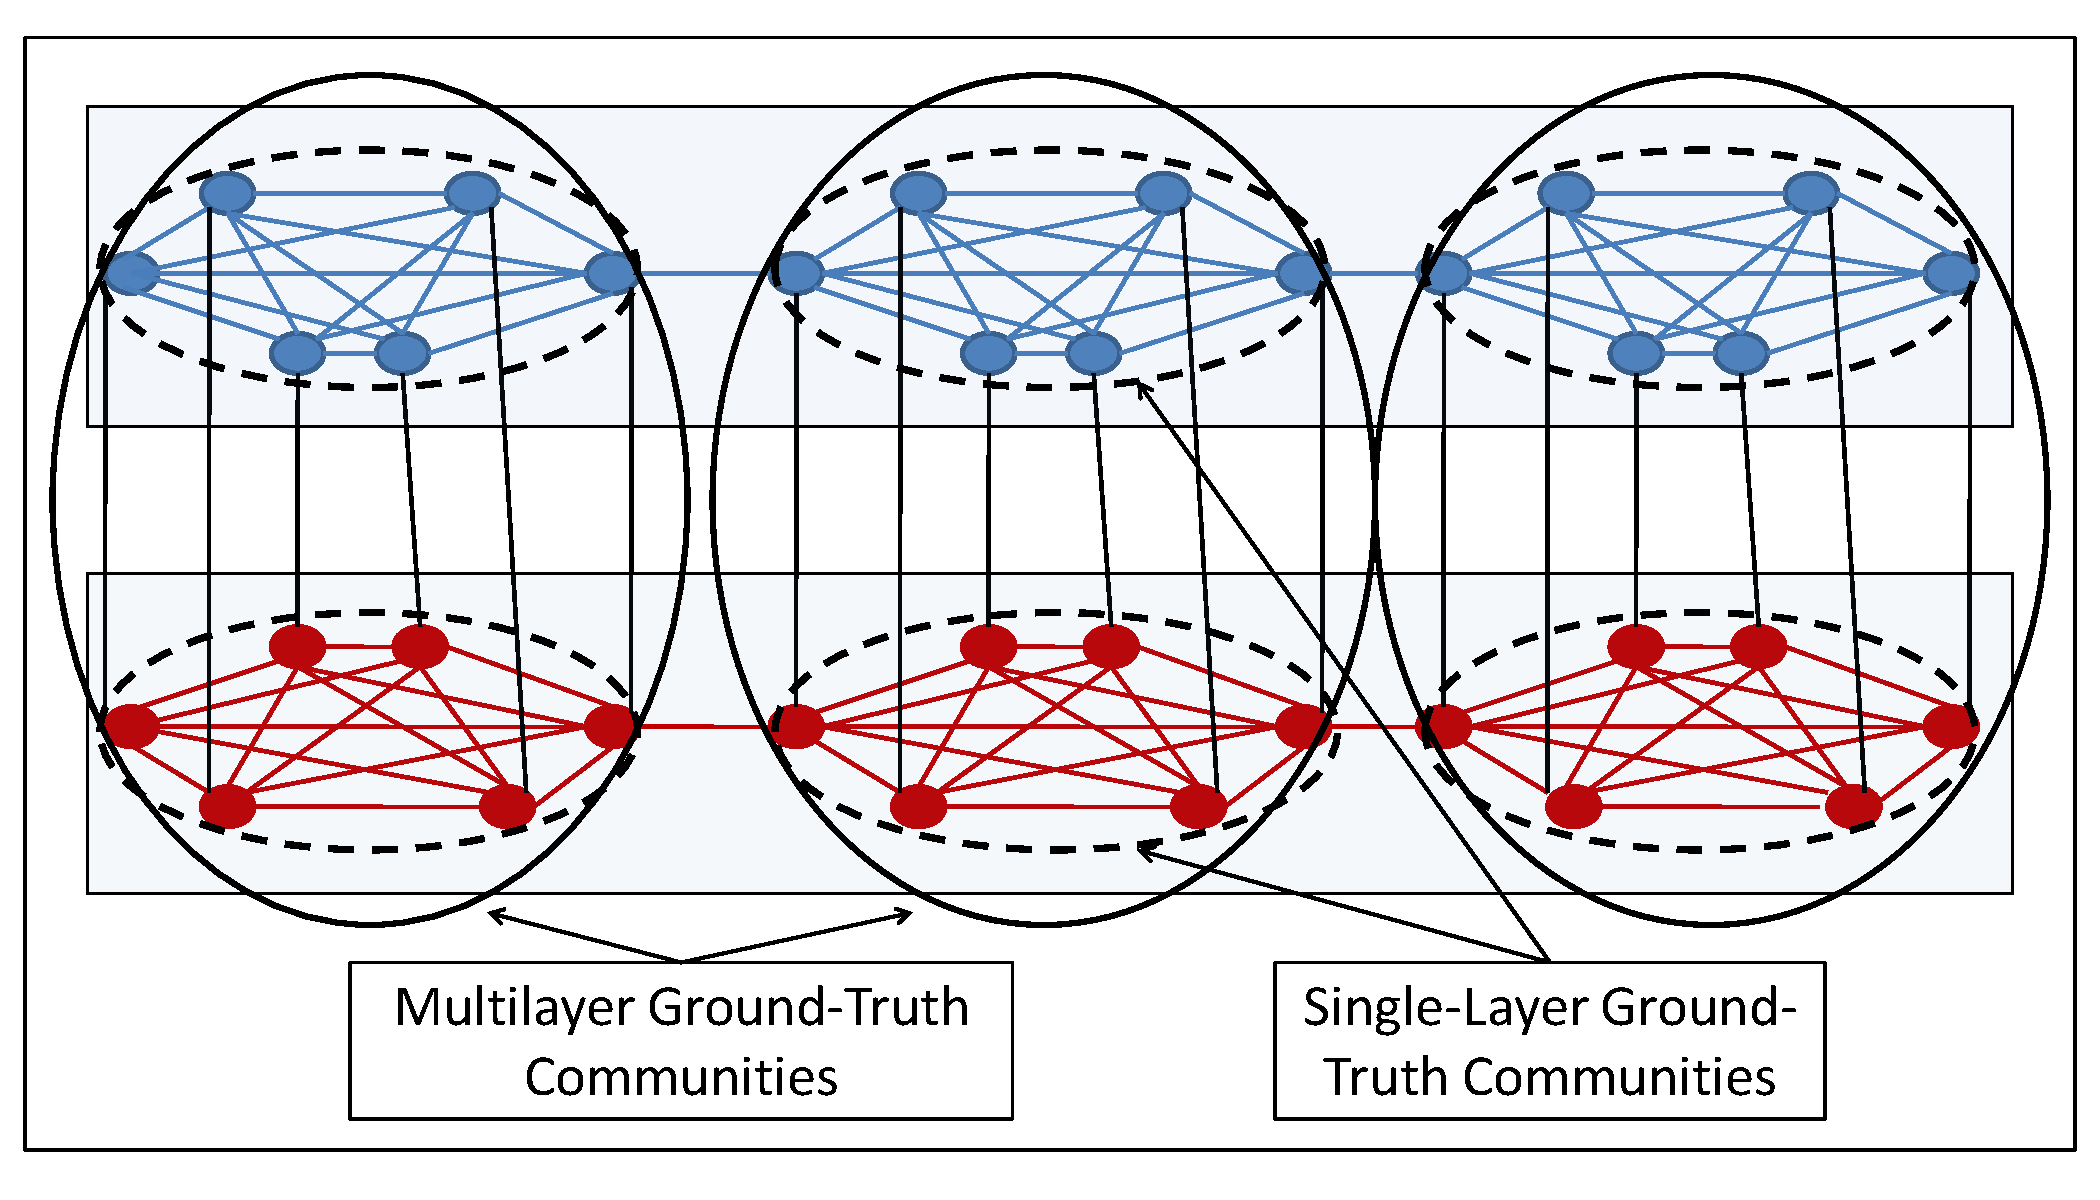
\includegraphics[width=3.5in]{./images/motivation.pdf}
\vspace{-0.1in}
\caption{Network configuration with two different ground truth communities}
\vspace{-0.1in}
\label{N0}
\end{figure}

% \begin{figure}
% \begin{center}
% \subfigure[Starting Configuration
% ]{\label{NN0}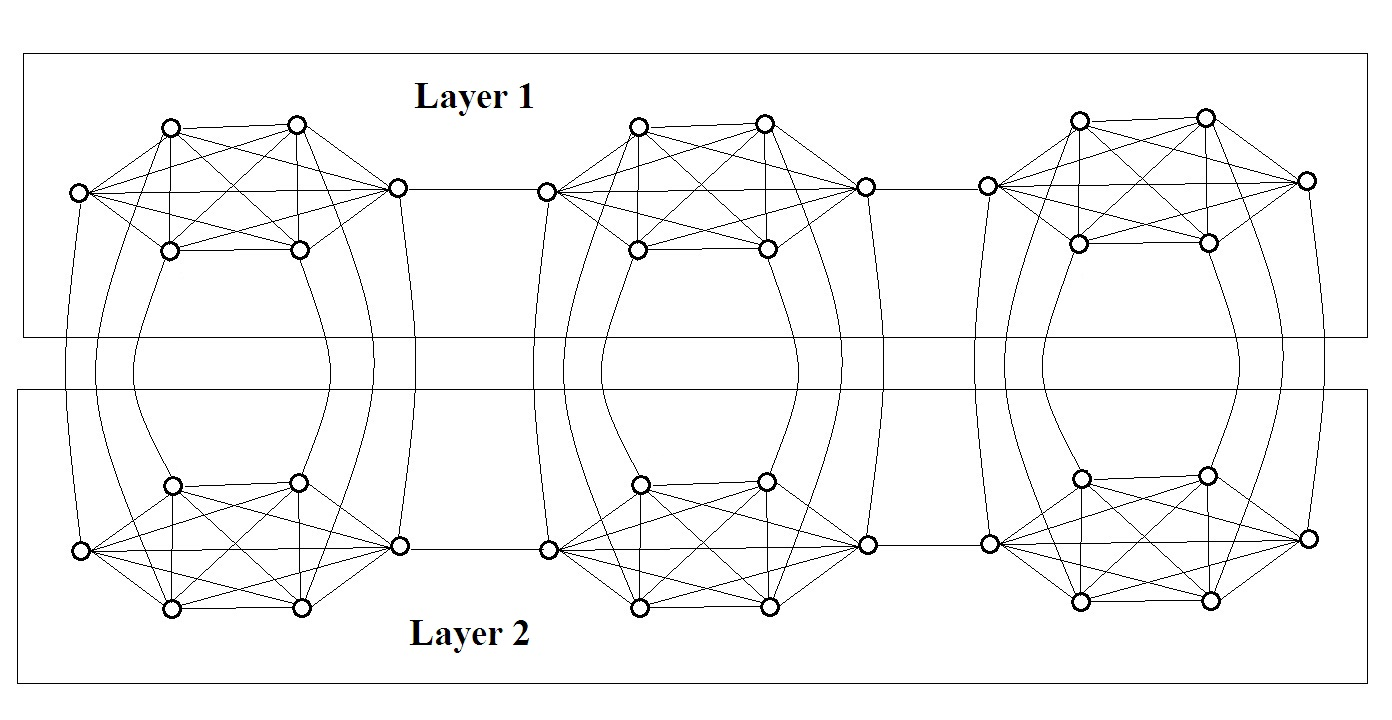
\includegraphics[angle=0,scale=.25]{./images/network0.jpg}}
% \subfigure[Ground Truth multilayer communities
% ]{\label{N01}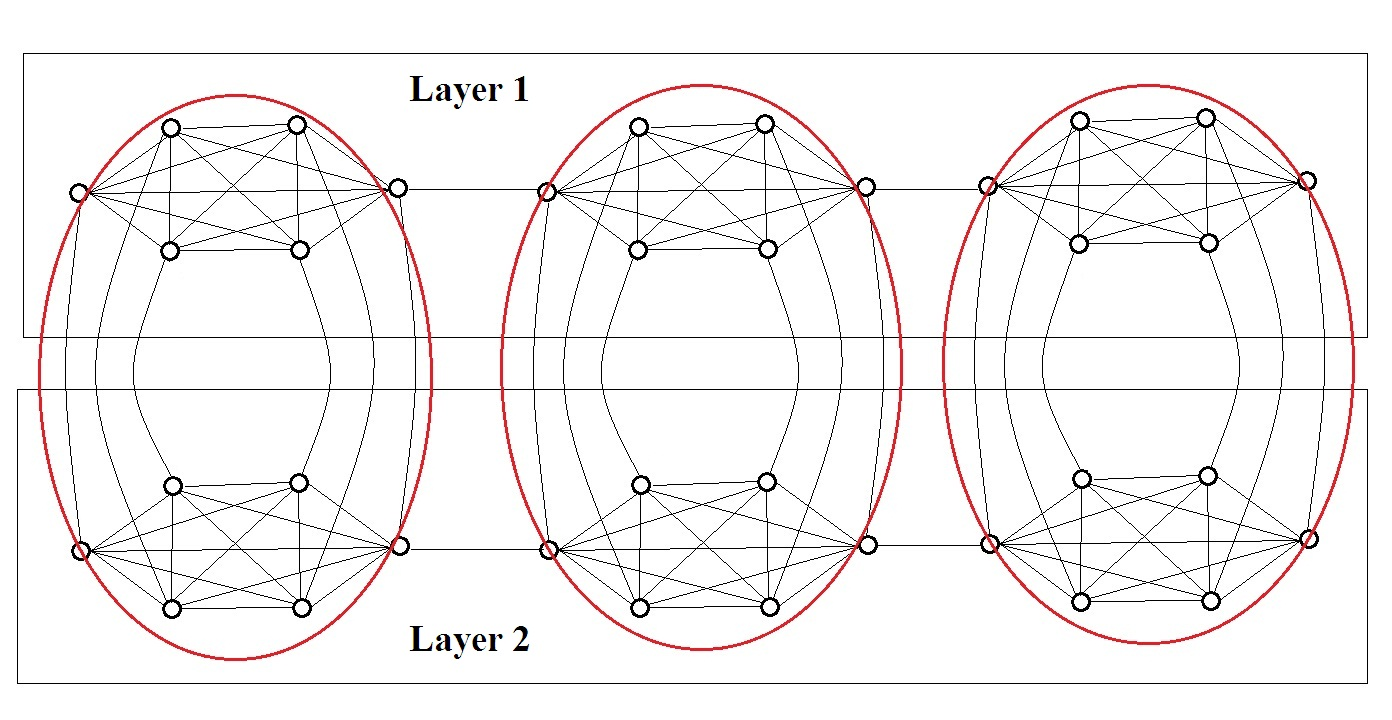
\includegraphics[angle=0,scale=.25]{./images/network0_1.jpg}}
% \subfigure[Ground Truth Single layer communities
% ]{\label{N02}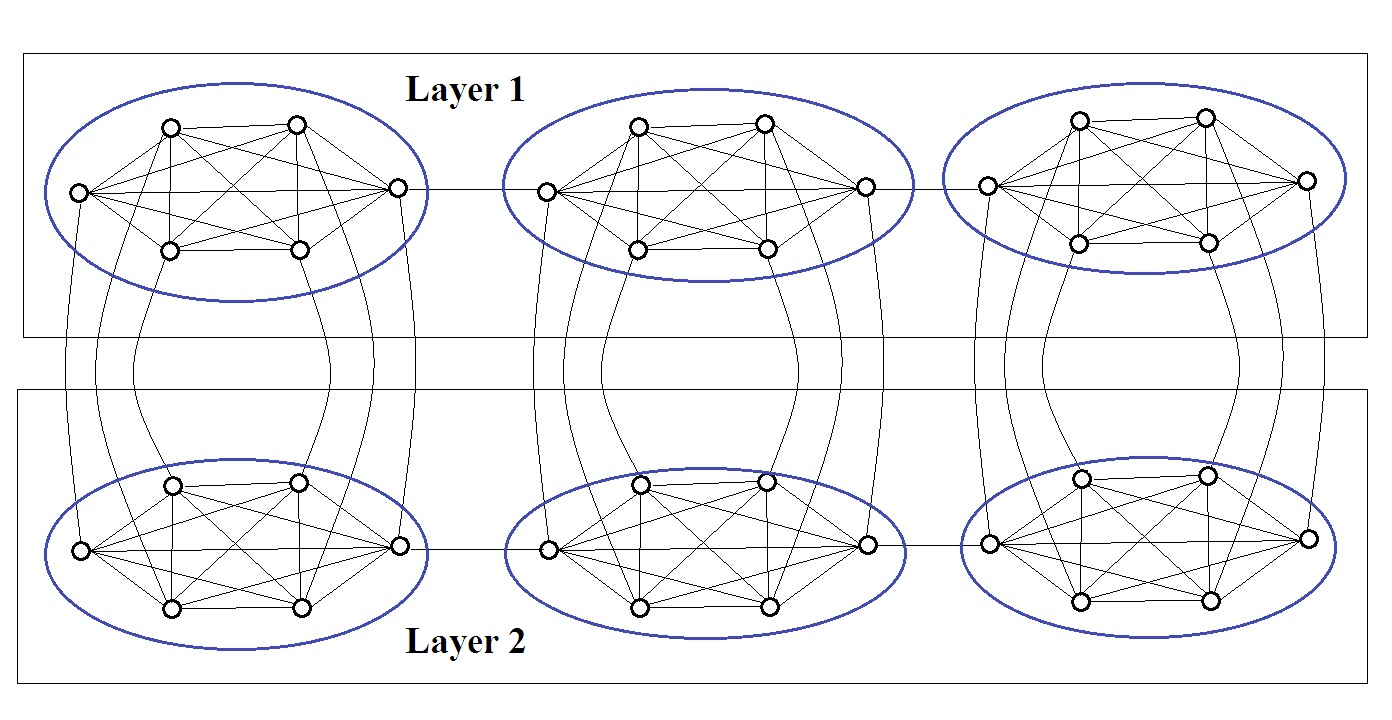
\includegraphics[angle=0,scale=.25]{./images/network0_2.jpg}}
% \end{center}
% \vspace{-0.22in}
% \caption{Network configuration with two different ground truth communities}
% \label{N0}
% \end{figure}



%Obviously, this modularity definition is not generic as it is defined for 2-layer networks only. 
The main deficiency of this definition comes from the fact that it checks the quality of a multilayer community 
by individually checking its 
single layer and bipartite components. It never checks how well the individual single layer components within each cross-layer community
are connected with each other.

For example, in Fig.~\ref{N0}, we show a two-layer network configuration with strong single layer modules (cliques of 100 nodes). 
There are same number of cliques (of same sizes) in both layers. Each clique in the top layer corresponds to exactly one clique in 
the bottom layer 
and there exists one-to-one coupling connections (total 300 coupling links) between the corresponding nodes.
We consider two different ground truth communities as shown in Fig.~\ref{N0} - one consisting of only single-layer communities 
(six in total), another 
consisting of only mixed communities (three in total).
If we gradually delete a fraction of coupling edges (randomly chosen), it is expected that the modularity corresponding 
to the multilayer ground truth would decrease and the modularity corresponding to single layer ground truth would 
increase. But, Fig.~\ref{mQ1} shows that 
none of this is actually captured by $mQ$. It throughout remains constant with coupling edge deletion. 
In case of multilayer communities it only decreases abruptly once all the coupling edges get deleted. 

\begin{figure}
\centering
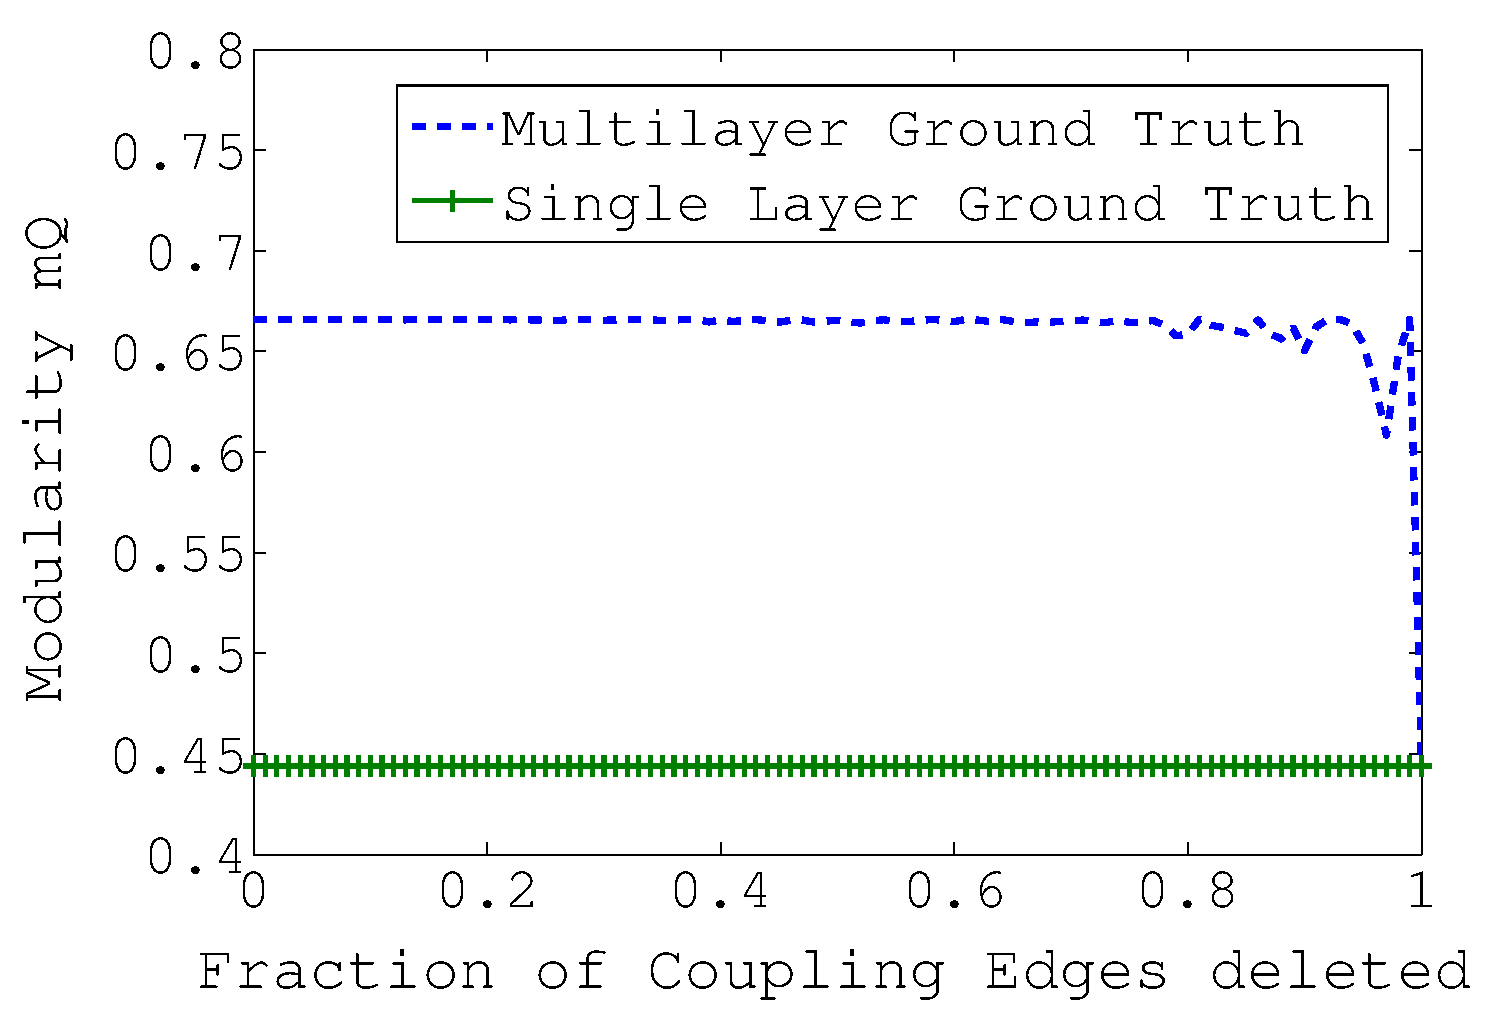
\includegraphics[width=2.5in]{./images/mQ_config1_2_100_5_no_ext_random_removal.pdf}
\vspace{-0.1in}
\caption{Change in mQ while deleting couplinng edges for both ground truth communities in Fig.~\ref{N0}}
\vspace{-0.1in}
\label{mQ1}
\end{figure}

The reason of this behaviour can be explained in the following way - in case of
single layer ground truth communities, the communities themselves do not include any coupling edge at all. So, in the calculation 
of modularity $mQ$, the coupling edges have no contribution and that is why $mQ$ remains constant even 
if more coupling edges get deleted.
On the other hand, for multilayer ground truth communities, each community has two single layer components and one coupling component.
The modularities of the single layer components do not change with coupling edge removal for the same reason stated above. 
But the bipartite modularity of the coupling component is expected to decrease with the deletion of coupling edges. 
Unfortunately, that does not happen. 
In our case, each coupling component is basically a set of parallel coupling edges.
When we remove the coupling edges, both numerator and denominator of the calculated bipartite modularity decreases (as there is no cross
community coupling edges) - essentially keeping
the total modularity sum almost constant.
% If there are E number of such edges in a multilayer community at any
% moment, the bipartite modularity of that component will 
% be $(E/(m*E)-(E*E)/(m*E)^2) = (1/m-1/m^2)$ where m is the number of multilayer communities ($m*E$ is the total number of coupling edges
% at this moment). 
So, the modularity of the coupling component of each community also becomes independent of the number of coupling edges present in the
network. This in turn makes the entire $mQ$ constant with respect to coupling edge deletion.
At the end when all the coupling edges get deleted, the bipartite modularity part of each community vanishes, resulting in a sudden drop in 
the total modularity.

In the next section, we propose our modularity metric which takes care of this limitations of $mQ$ by increasing its sensitivity about
how well the coupling links connect individual single layer components in each multilayer community.
% In Fig.~\ref{NN}, we show another network configuration with almost same configuration as Fig.~\ref{NN0} except that here 
% we have a strongly connected bipartite portion attached with each single layer clique. Similar to previous case,
% we consider two different ground truth communities as shown in Fig.~\ref{N01} and Fig.~\ref{N02}.
% If we gradually delete the coupling edges (except the ones in the bipartite clique part) one by one, 
% it is expected that the modularity corresponding to multilayer ground truth 
% should decrease and the modularity corresponding to single layer ground truth should increase. 
% Fig.~\ref{mQ2} shows that in this case also, the metric mQ is not sensitive to the quality of the multilayer communities.
% This happens because of the same reason as in the case of configuration 1. The modularities of single layer components of each 
% multilayer community do not get affected by the deletion of coupling edges. Only the bipartite modularity of the coupling portion 
% could have got affected. But unfortunately it doe not. Suppose, we have E number of coupling edges in a multilayer community at a 
% point of time other than the 5*5 dense bipartite portion. 
% Then the bipartite modularity of that coupling component of the community would 
% be $((E+25)/(m*(E+25))-((E+25)*(E+25))/(m*(E+25))^2) = (1/m-1/m^2)$ 
% where m is the number of multilayer communities ($m*(E+25)$ is the total number of coupling edges
% at this moment). So, here also, this factor is independent of the number of coupling edges present. 
% That is why the overall modularity of the multilayer communities does not change even if we delete coupling edges gradually.
% 
% In case of single layer ground truth communities, there is a difference from the result of configuration 1, due to the presence of 
% 5*5 strongly connected bipartite communities. As the total number of coupling edges (which is in the denominator 
% of the bipartite modularity definition) decrease at every step, the modularities of those three 5*5 communities improve. 
% The modularities of other six purely single layer 
% communities do not vary with coupling edge deletion. So, overall $mQ$ of the network increases with coupling edge deletion i.e.
% the metric is able to detect changes with respect to the single layer ground truth in case of configuration 2.
% 
% 
% 
% \begin{figure}
% \begin{center}
% \subfigure[Starting Configuration
% ]{\label{NN}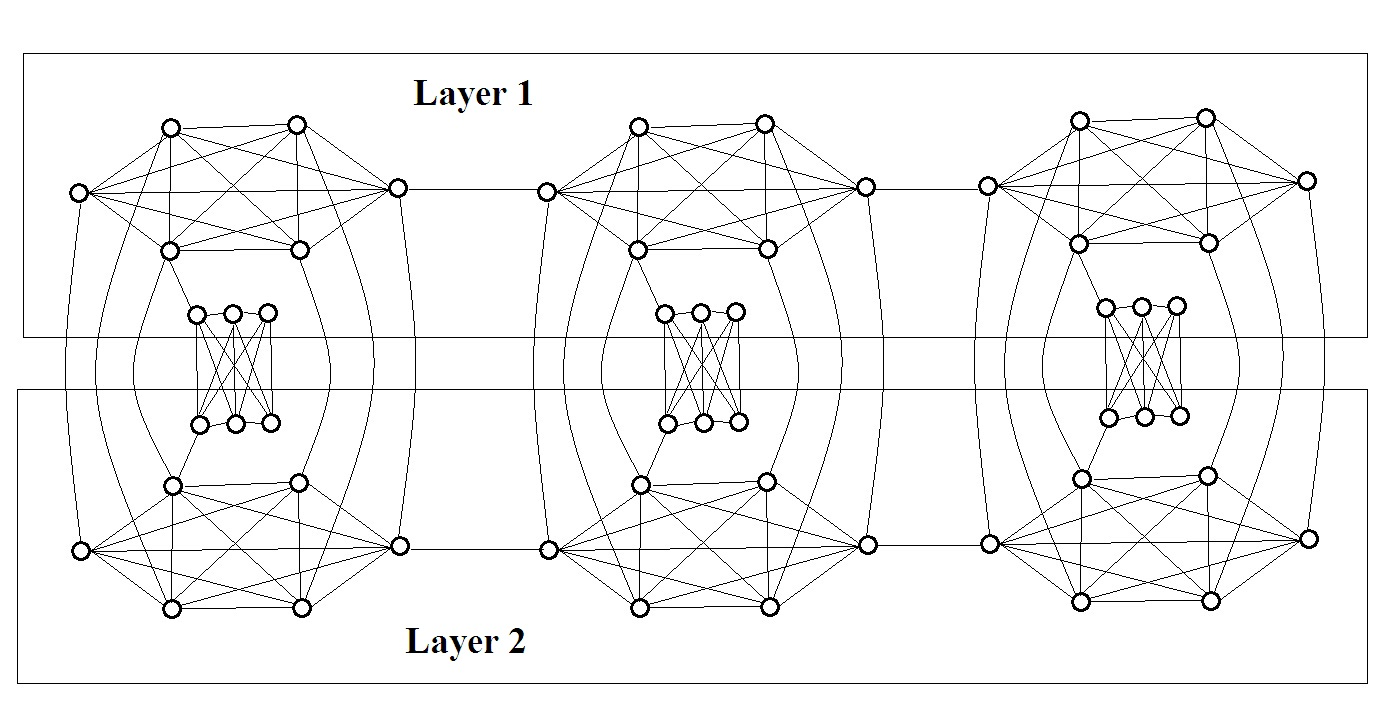
\includegraphics[angle=0,scale=.3]{./images/network.jpg}}
% \subfigure[Ground Truth multilayer communities
% ]{\label{N1}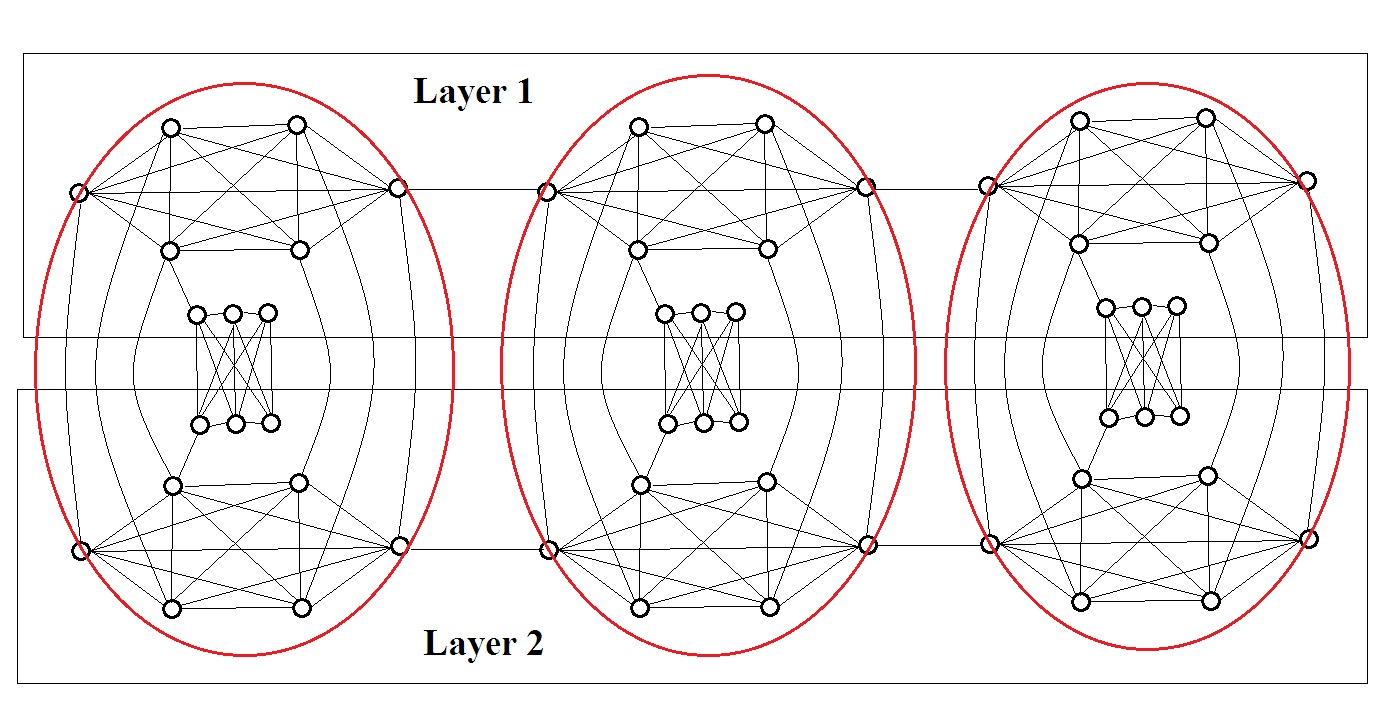
\includegraphics[angle=0,scale=.3]{./images/network1.jpg}}
% \subfigure[Ground Truth Single layer communities
% ]{\label{N2}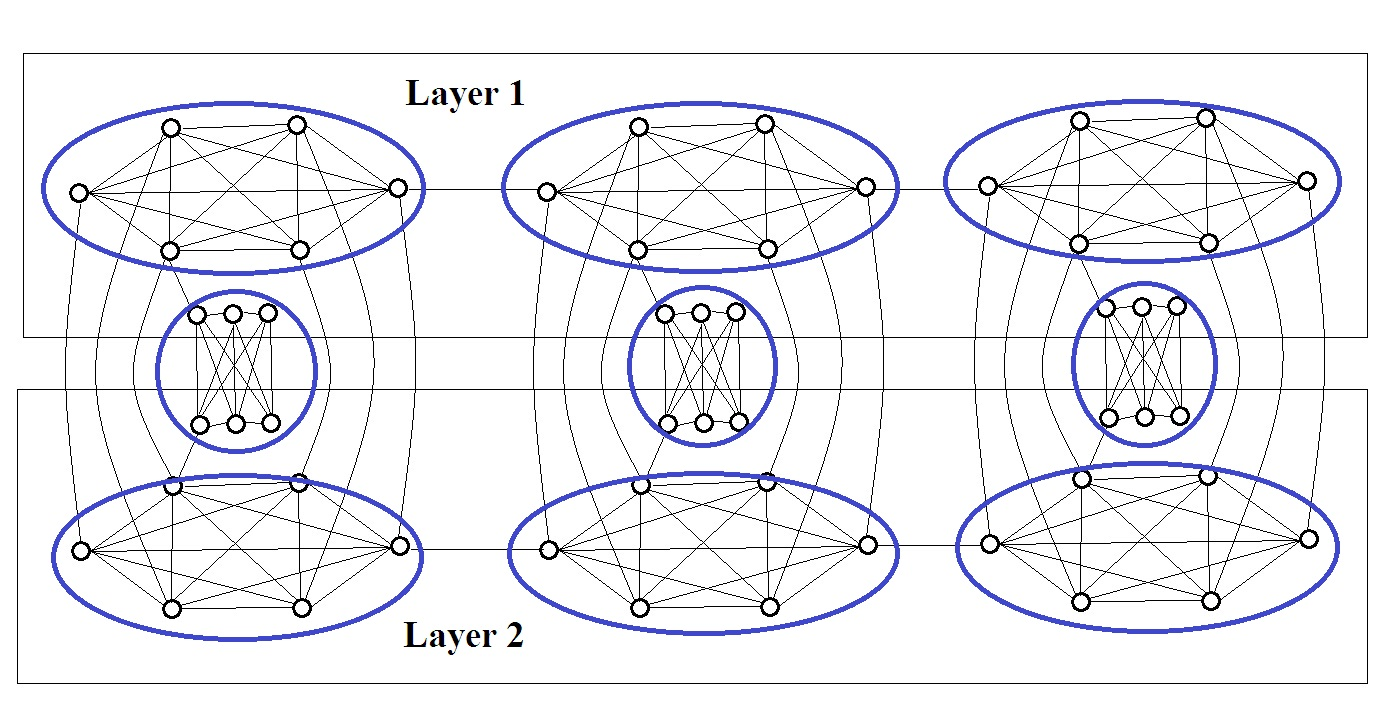
\includegraphics[angle=0,scale=.3]{./images/network2.jpg}}
% \end{center}
% \vspace{-0.22in}
% \caption{Network configuration 2 with two different ground truth communities}
% \label{N}
% \end{figure}
% 
% \begin{figure}
% \centering
% 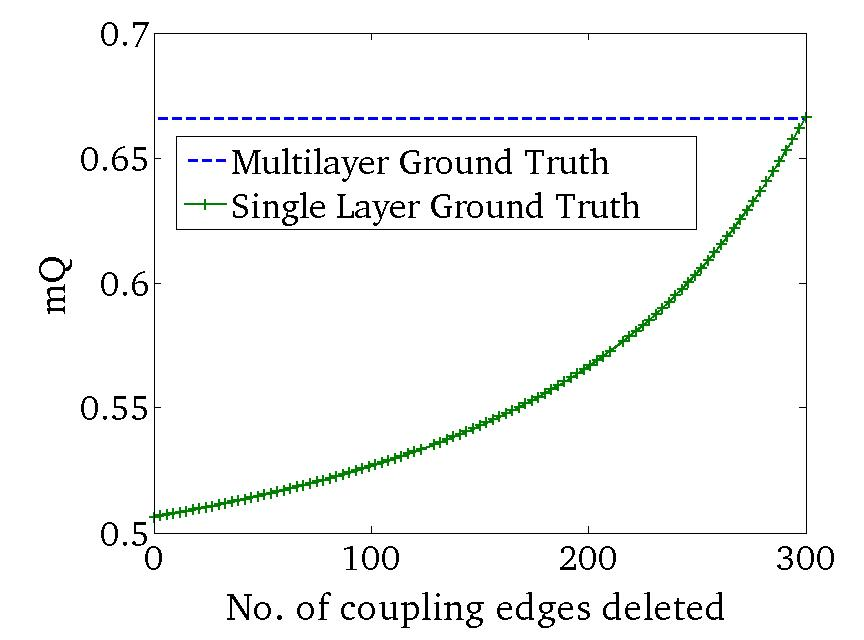
\includegraphics[width=2.5in]{./images/mQ_config1_2_100_5.jpg}
% \vspace{-0.1in}
% \caption{Change in mQ while deleting coupling edges for both ground truth communities in configuration 2}
% \vspace{-0.1in}
% \label{mQ2}
% \end{figure}
% 
% \textcolor{red}{[SP: We should try to generalize more on the limitation of $mQ$. To emphasize the superiority of our metric - 
% Is it enough to show that $mQ$ is not sensitive to a particular type of networks (as generic as possible) and 
% sensitive to other types of networks whereas our metric is sensitive to all types of networks?\\
% Can we get an idea from the configurations 1\& 2 here, about how to modify $Q_{adapt}$? We can also consider the weighted version of 
% $mQ$ with different weightages to single layer and cross-layer components.]
% }

\section{Developing multilayer community detection algorithm}
\label{metric}
In this section, first we develop the modularity index $Q_M$ to characterize the quality of multilayer communities. Next, we show
that simple adaptation of $Q_M$ with classical methodologies may lead to the development of multilayer community detection algorithms.

%the way we combine it with existing single layer community detection algorithms to detect multilayer communities.
% \begin{figure*}
% \centering
% 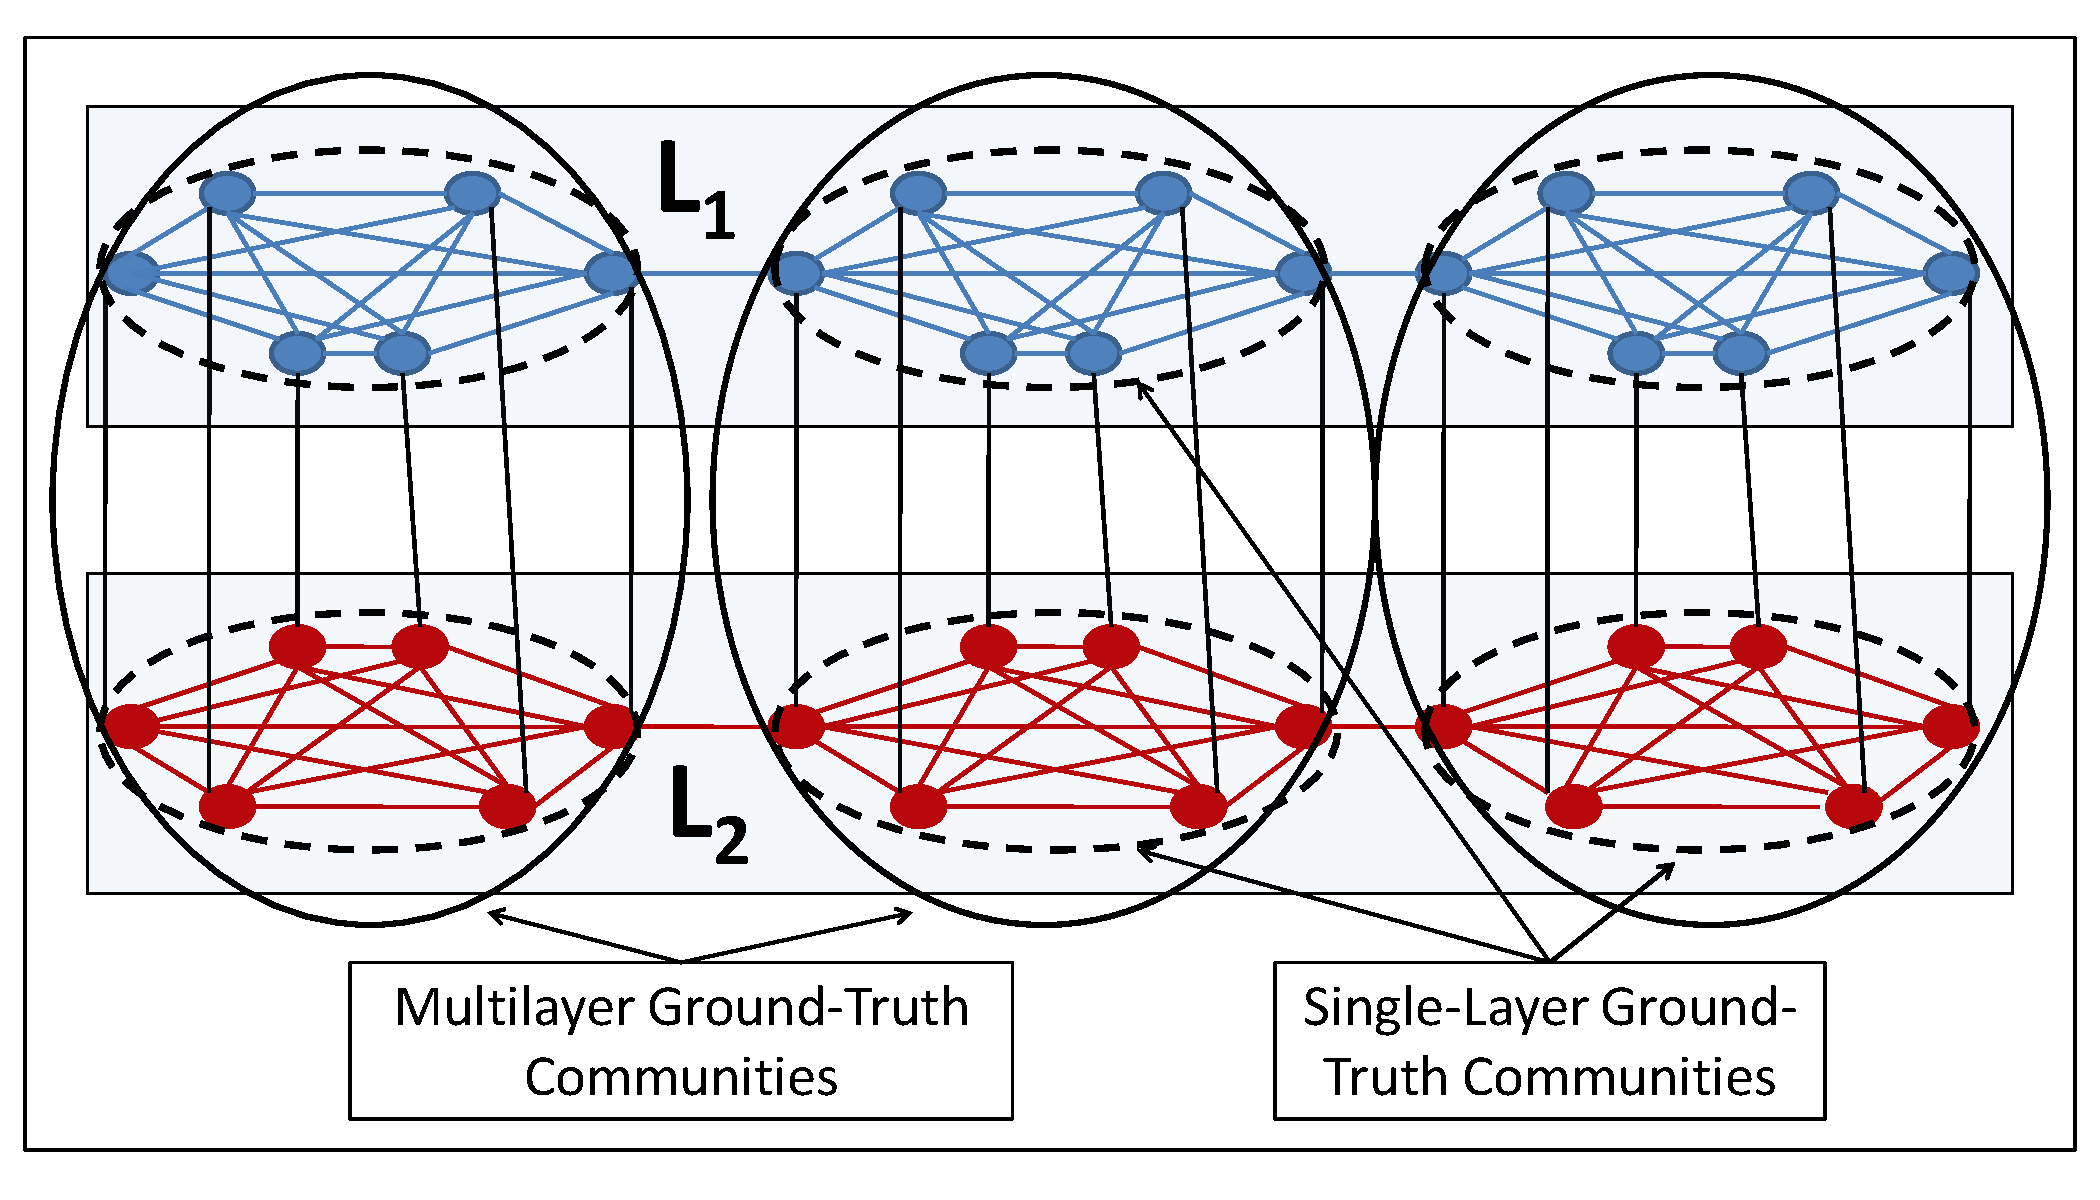
\includegraphics[width=3.5in]{./images/image31.pdf}
% \vspace{-0.2in}
% \caption{Network configuration with two different ground truth communities}
% \vspace{-0.2in}
% \label{N0}
% \end{figure*}

% \begin{figure}
% \centering
% 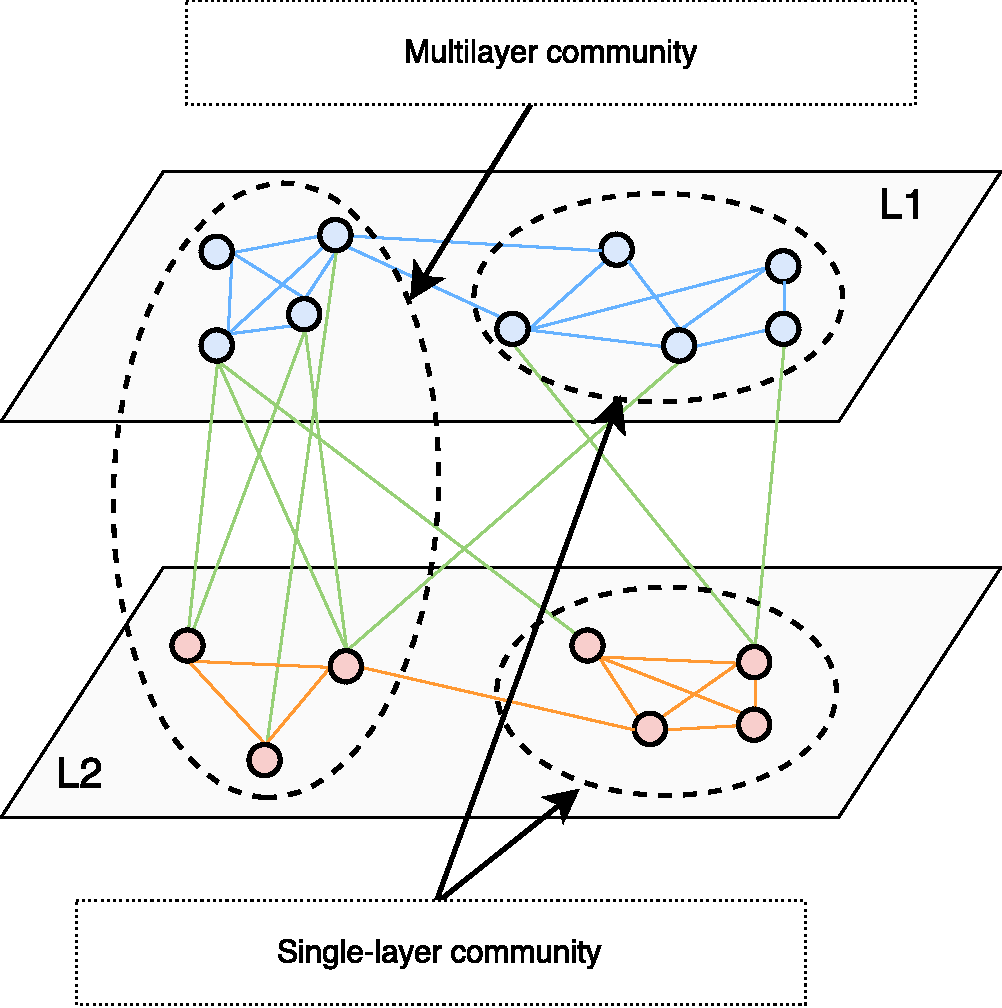
\includegraphics[width=2in]{./images/single_multi_community.pdf}
% \vspace{-0.1in}
% \caption{A sample multilayer network with two different types of communities}
% \label{mul_comm}
% \end{figure}

\subsection{Desired properties of multilayer communities: Intuition}\label{prop}
We start this section highlighting the desired properties of the communities in a multilayer network.
As introduced in section~\ref{dataset}, in multilayer networks, we observe two types of communities (see Fig.~\ref{N0})
(a) cross layer communities (containing multiple types of nodes) and
(b) single layer communities (containing only single type of nodes).

For an `ideal' cross layer community $C = (\mathcal{C_U},\mathcal{C_B})$ of $\mathcal{G}$
(where $\left \vert \mathcal{C_B} \right \vert \neq \Phi$), the desired properties are the following,

\textbf{$Property^{X1}:$} The group of nodes in each uni-partite and bipartite layer ($L^C_i$s and $L^C_{ij}$s respectively) should 
be highly cohesive.

\textbf{$Property^{X2}:$} The (coupling) edges in the bipartite layer $L^C_{ij} \in \mathcal{C_B}$ should connect most of the nodes
from $L^C_i$ (i.e. $V^C_i$) with most of the nodes from $L^C_j$ (i.e. $V^C_j$).

%For each pair of $(L^C_i, L^C_j) \in \mathcal{C_U}$,

Similarly, for an `ideal' single layer community $C= (\mathcal{C_U},\mathcal{C_B})$ of $\mathcal{G}$ (where
$\mathcal{C_B} = \Phi$), the desired properties are enumerated below,

\textbf{$Property^{S1}:$} The community should be highly cohesive within the layer $L_i$ to which it
belongs (i.e. $\mathcal{C_U} = L^C_i \subseteq L_i$).

\textbf{$Property^{S2}:$} The nodes in $L^C_i$ (i.e. $V^C_i$) should be very loosely connected with nodes of other layers $L_j$.

%\vspace{-0.4in}
\subsection{Multilayer Modularity Index}\label{mult_mod}
Following the aforesaid intuitions, we propose multilayer modularity for a two-layer network
$\mathcal{G} = \{\{L_1, L_2\}, \{L_{12}\}\}$
where $L_1$ = ($V_1$, $E_1$) \& $L_2$ = ($V_2$, $E_2$) are the individual layers
and $L_{12}$ = ($V_1$, $V_2$, $E_{12}$) is the bipartite graph connecting nodes of layer $L_1$ and $L_2$.

We start with the basic notion of Newman-Girvan modularity~\cite{newman2006modularity},
$Q = \frac{1}{2m}\sum_{i,j} (A_{ij} - P_{ij})\delta(\psi_i,\psi_j)$ where $m$
%$= \left \vert E_1 \right \vert + \left \vert E_2 \right \vert + \left \vert E_{12} \right \vert$
is the total number of edges in the network, $i,j \in V_1 \cup V_2$ are any pair of nodes in the
network, $\psi_i$ indicates the community membership of node $i$ and $\delta(\psi_i,\psi_j)$ is the Kronecker delta function which
is $1$ only if $\psi_i=\psi_j$ i.e. $i$ and $j$ belong to the same community (and $0$ otherwise).
%[BM: notational inconsistency with $c_i$, community or coupling degree?]
$A_{ij}$ represents the classical adjacency matrix of $\mathcal{G}$. The penalty term $P_{ij}$ (often referred as null model)
is the expected probability of having an edge between nodes $i$ and $j$ if edges are placed at random.
Notably, in multilayer network the edges in one layer $L_i$ are intrinsically different from another layer $L_j$, which gets
reflected in the property of the corresponding layers as well (say diverse edge densities across the layers). This observation motivates
us to introduce layer-wise discriminating null models, and propose the following
multilayer modularity, %[BM: try if this can be part of Eq 1] $Q_M= \frac{1}{2m}\sum_{ij}\{(A_{ij}-P_{ij})\delta(\psi_i,\psi_j)\}~where$
\vspace{-0.1in}
\begin{dmath}\label{eq11}
{Q_M = \frac{1}{2m}\sum_{ij}\{(A_{ij}-P_{ij})\delta(\psi_i,\psi_j)\} ~where}\\
{P_{ij}=\left\{ \begin{array}{ll}
                  P^1_{ij}~~if~i \in V_1~\&~j \in V_1\\
                  P^2_{ij}~~if~i \in V_2~\&~j \in V_2\\
                  P^{12}_{ij}~~if~(i \in V_1~\&~j \in V_2)~or~(i \in V_2~\&~j \in V_1)
                \end{array}
              \right.}
\end{dmath}
\vspace{-0.15in}
In the following, we compute the null model terms $P^1_{ij}$, $P^2_{ij}$ and $P^{12}_{ij}$ separately for both types
of communities of multilayer network and finally derive the multilayer modularity index $Q_M$.
%in a way that imposes our desired behaviours (as discussed in the previous subsection) on them.
% As mentioned before, we have a very different set of expectations from a cross layer community than a single layer one.
% Due to this fact, the $P^1_{ij}$, $P^2_{ij}$ and $P^{12}_{ij}$ terms have to be defined separately for both type of communities.

\subsubsection{Cross Layer Communities}
Any cross layer community $C$ is composed of three submodules - two intra layer ($L^C_1$, $L^C_2$) and one inter layer ($L^C_{12}$).
The vanilla null model proposed in~\cite{newman2006modularity} directly derives the $P^1_{ij}$, $P^2_{ij}$ for intra layer submodules.
The expected number of edges between any two nodes $i$ and $j$ (with intra-layer degrees
$h_i$ and $h_j$ respectively) within the community $C$ can be calculated as
$P^1_{ij}=(h_i*h_j)/2\left \vert E_1 \right \vert$ (for submodule $L^C_1$) and $P^2_{ij}=(h_i*h_j)/2\left \vert E_2 \right \vert$
(for submodule $L^C_2$).
%This is essentially the same classic null model proposed by Newman~\cite{newman2006modularity}.
For inter layer or bipartite submodule $L^C_{12}$, the probability of an edge between node $i$ and $j$ depends on their respective
coupling degrees $c_i$ and $c_j$.
%not only depends on their degrees in the corresponding coupling layer but
%also on their individual intra-layer degrees.
The probability of having a coupling edge between $i$, $j$ can be estimated as $P^{12}_{ij}=(c_i*c_j)/\left \vert E_{12} \right
\vert$ (similar
to~\cite{barber2007modularity}). The aforementioned null models satisfy the desired requirements of $Property^{X1}$ introduced
in section~\ref{prop}.
%[SP:SHOULD I REFER BARBAR's MODULARITY?].

Each cross layer community $C$ is represented as $\{\{L^C_1, L^C_2\}, \{L^C_{12}\}\}$ where
$L^C_1$ and $L^C_2$ are the submodules with edges from $E_1$ and $E_2$ respectively and $L^C_{12}$ is from $E_{12}$;
we substitute $P_{ij}$ in Eq.~\ref{eq11} to define its modularity as
\vspace{-0.1in}
\begin{dmath}\label{eq_mid}
Q_M^C= {\forall i,j \in C}~ \left[ \frac{1}{3} \bigg \{
 \frac{1}{2\left \vert E_1 \right \vert}
 \sum_{i,j \in V_1}\big(A_{ij} - \frac{ (h_i * h_j)}{2\left \vert E_1 \right \vert}\big) +
 \frac{1}{\left \vert E_{12} \right \vert}
 \sum_{i \in V_1, j \in V_2}\big(A_{ij} - \frac{ (c_i * c_j)}{\left \vert E_{12} \right \vert}\big) +
 \frac{1}{2\left \vert E_{2} \right \vert}
 \sum_{i,j \in V_2}\big(A_{ij} - \frac{ (h_i * h_j)}{2\left \vert E_2 \right \vert}\big)
    \bigg \}\right]
\end{dmath}
\vspace{-0.08in}
% Q_M^C= \forall i,j \in C~ \{\frac{1}{3}\{(\frac{\sum_{i,j \in V_1} A_{ij}}{2*\left \vert E_1 \right \vert} -
%  \frac{\sum_{i,j \in V_1} (h_i * h_j)}{(2*\left \vert E_1 \right \vert)^2}) +
%  (\frac{\sum_{L(i) \neq L(j)} A_{ij}}{2*\left \vert E_{12} \right \vert} -
%  \frac{\sum_{L(i) \neq L(j)} (c_i * c_j)}{2*\left \vert E_{12} \right \vert^2}) +
%  (\frac{\sum_{i,j \in V_2} A_{ij}}{2*\left \vert E_2 \right \vert} -
%  \frac{\sum_{i,j \in V_2} (h_i * h_j)}{(2*\left \vert E_2 \right \vert)^2})\}\}
%where $L(i)=l$ if vertex $i$ belongs to layer $l$.
%[BM: be consistent in the terminologies. intra-layer submodule or bipartite submodule? edge/edges etc]
% \begin{dmath}
% OR,~Q_M^C= \forall i,j \in C~ \{\frac{1}{3}\{(\frac{\sum_{i,j \in V_1} A_{ij}}{2*\left \vert E_1 \right \vert} -
%  \frac{(\sum_{i \in V_1} h_i) * (\sum_{j \in V_1} h_j)}{(2*\left \vert E_1 \right \vert)^2}) +
%  (\frac{\sum_{i \in V_1 j \in V_2} A_{ij}}{\left \vert E_{12} \right \vert} -
%  \frac{(\sum_{i \in V_1} c_i) * (\sum_{j \in V_2} c_j)}{(\left \vert E_{12} \right \vert)^2}) +
%  (\frac{\sum_{i,j \in V_2} A_{ij}}{2*\left \vert E_2 \right \vert} -
%  \frac{\sum_{i \in V_2} h_i * \sum_{j \in V_2} h_j}{(2*\left \vert E_2 \right \vert)^2})\}\}
% \end{dmath}
%[BM: one sum per layer.]
In case of inter layer submodule, if node $i$ in $C$ is not connected with any other layer (hence, coupling degree $c_i$ zero), we
use its intra layer degree $h_i$ as a proxy of $c_i$ for computing $P^{12}_{ij}$. This allows us to penalize those
nodes in cross layer community $C$ which are only connected with
nodes within the same layer and \emph{not} with the nodes in $C$ of different layer. This amendment in the null
model $P^{12}_{ij}$ satisfies the desired requirements of $Property^{X2}$. Therefore with this modification, the Eq.~\ref{eq_mid}
can be written as,
\vspace{-0.08in}
\begin{dmath}\label{eq_multi}
Q_M^C= {\forall i,j \in C}~  \left[ \frac{1}{3}\bigg \{
 \frac{1}{2\left \vert E_1 \right \vert}
 \sum_{i,j \in V_1}\big(A_{ij} - \frac{ (h_i * h_j)}{2\left \vert E_1 \right \vert}\big) +\\
 {\frac{1}{2\left \vert E_1 \right \vert + 2\left \vert E_2 \right \vert + \left \vert E_{12} \right \vert}
 \sum_{i \in V_1, j \in V_2}\big(A_{ij} - \frac{ ({c'}_i * {c'}_j)}
 {2\left \vert E_1 \right \vert + 2\left \vert E_2 \right \vert + \left \vert E_{12} \right \vert}\big)} +
 \frac{1}{2\left \vert E_{2} \right \vert}
 \sum_{i,j \in V_2}\big(A_{ij} - \frac{ (h_i * h_j)}{2\left \vert E_2 \right \vert}\big)
   \bigg \}\right]
\end{dmath}
\vspace{-0.08in}
where for any node $i$, ${c'}_i=c_i$ if $c_i > 0$ and ${c'}_i=h_i$ otherwise.
% [BM: rewrite the following sentence?? I tried once.]
% Finally, summing over all node pairs in the community $C$ following Eq.~\ref{eq_mid},
% \begin{dmath}\label{cross1}
% Q_M^C= \{\frac{1}{3}\{\underbrace{[\frac{\left \vert E^C_1 \right \vert}{\left \vert E_1 \right \vert}-
%  (\frac{d^C_1}{2*\left \vert E_1 \right \vert})^2]}_{Term~ for~ Single~ Layer~ L_1}
%  +\underbrace{[\frac{\left \vert E^C_{12} \right \vert}{\left \vert E_{1} \right \vert + \left \vert E_{2} \right \vert + \left \vert E_{12} \right \vert}-
%  \frac{k^C_{12}*{d^C_{12}}}{{(2*\left \vert E_{1} \right \vert + 2*\left \vert E_{2} \right \vert + \left \vert E_{12} \right \vert)}^2}]}_{Term~ for~ Coupling~ edges}
%  +\underbrace{[\frac{\left \vert E^C_2 \right \vert}{\left \vert E_2 \right \vert}-(\frac{d^C_2}{2*\left \vert
%  E_2 \right \vert})^2]}_{Term~ for~ Single~ Layer~ L_2}\} \}
% \end{dmath}
% where $\left \vert E^C_1 \right \vert$, $\left \vert E^C_2 \right \vert$ \& $\left \vert E^C_{12} \right \vert$ are the number of edges
% present in community $C$ from layers $L_1$, $L_2$ and $L_{12}$; $d^C_1$ ($d^C_2$) is the sum of intra-layer degrees of
% all $L^C_1$ ($L^C_2$) nodes in $L_1$ ($L_2$) layer;
% $k^C_{12}$ and $d^C_{12}$ [BM: change the symbols $k, d$] are the sum of coupling degrees (with suitable proxies)
% of $L^C_1$ and $L^C_2$ nodes respectively.

%and $d^C_{12}$ is the sum of coupling degrees of $L^C_2$ nodes.
%in subnetwork $L_{12}$.


\subsubsection{Single Layer Communities}
In any single layer community $C$, all the constituent nodes belong to either $L_1$ or $L_2$. The null models
can be directly derived as $P^1_{ij}=(h_i*h_j)/2\left \vert E_1 \right \vert$ and $P^2_{ij}=(h_i*h_j)/2\left \vert E_2 \right \vert$ for
layer $L_1$ and $L_2$ respectively from the vanilla null model~\cite{newman2006modularity}. These null models satisfy
the $Property^{S1}$ introduced in section~\ref{prop}.
Hence, for each single layer community $C$ represented as $\{L^C_1\}$,
we substitute $P_{ij}$ in Eq.~\ref{eq11} to compute the modularity as,
\vspace{-0.05in}
\begin{dmath}
Q_M^C={\forall i,j \in C} \left [ \frac{1}{3} \bigg \{
\frac{1}{2\left \vert E_1 \right \vert} \sum_{i,j \in V_1}
\big(A_{ij} -
\frac{(h_i * h_j)}{2\left \vert E_1 \right \vert}\big) \bigg \} \right]  \end{dmath}
\vspace{-0.05in}
Importantly, there can be many nodes in $C$ which are connected to other layer nodes via coupling edges,
violating $Property^{S2}$ of desired single layer community.
%one of our desired criteria (loose coupling with nodes from the other layer) for an `ideal' single layer community.
In order to penalize those nodes in a community $C$ with coupling
degree $c_i$, we add $c_i$ along with $h_i$ to estimate the null model.
Subsequently, the modularity of $C$ becomes
%After taking care of the coupling degrees of nodes in a single layer community,
\vspace{-0.05in}
\begin{dmath}\label{eq_single}
{Q_M^C=\forall i,j \in C}~ \penalty0{\left[ \frac{1}{3} \bigg \{
\frac{1}{2\left \vert E_1 \right \vert+\left \vert E_{12} \right \vert} \sum_{i,j \in V_1}
\big(A_{ij} - \penalty0
\frac{(h_i+c_i) * (h_j+c_j)}{2\left \vert E_1 \right \vert+\left \vert E_{12} \right \vert}\big) \bigg \}
\right]}
\end{dmath}
\vspace{-0.08in}
% Q_M^C=\forall i,j \in C~ \{\frac{1}{3}(\frac{\sum_{i,j \in V_1} A_{ij}}{2*\left \vert E_1 \right \vert+\left \vert E_{12} \right \vert} -
%  \frac{\sum_{i,j \in V_1} ((h_i+c_i) * (h_j+c_j))}{(2*\left \vert E_1 \right \vert+\left \vert E_{12} \right \vert)^2}) \}

%This reflects the fact that a node with high coupling degree can only be a part of a single layer community if it contributes even higher number of edges within the community which essentially imposes our desired criteria.

%Notably, it is not required to add this type of coupling degree terms while calculating single layer modularities of cross layer communities because Eq.~\ref{cross1} already has a bipartite term to take care of them judiciously.

% \begin{dmath}
% OR,~Q_M^C= \forall i,j \in C~ \{\frac{1}{3}(\frac{\sum_{i,j \in V_1} A_{ij}}{2*\left \vert E_1 \right \vert+\left \vert E_{12} \right \vert} -
%  \frac{(\sum_{i \in V_1} (h_i+c_i)) * (\sum_{j \in V_1} (h_j+c_j))}{(2*\left \vert E_1 \right \vert+\left \vert E_{12} \right \vert)^2}) \}
% \end{dmath}
% But they may or may not be connected
% with other layer vertices via coupling edges. So, the expected number of edges between $i$ and $j$ with intra-layer degrees
% $h_i$ \& $h_j$ and coupling degrees $c_i$ \& $c_j$ can be calculated as
% $((h_i+c_i)*(h_j+c_j))/2\left \vert E_1 \right \vert$ or $((h_i+c_i)*(h_j+c_j))/2\left \vert E_2 \right \vert$ depending on whether
% the community is in layer 1 or layer 2.
% Finally, summing over all node pairs in the community $C$ following Eq. XX [BM: replace],
% \begin{dmath}
% Q_M^C= \{\frac{1}{3}(\frac{\left \vert E^C_1 \right \vert}{\left \vert E_1 \right \vert+ \left \vert E_{12} \right \vert/2}-
%  (\frac{{d'}^C_1}{2*\left \vert E_1 \right \vert+\left \vert E_{12} \right \vert})^2) \}
% \end{dmath}
% where $\left \vert E^C_1 \right \vert$ is the number of intra community edges and ${d'}^C_1 = {d}^C_1 + {CO}^C_1$ is the sum of intra-layer (${d}^C_1$) and coupling (${CO}^C_1$) degrees of
% all $L^C_1$ nodes in $L_1$ layer. Similar expression can be derived if $C$ is a submodule of $L_2$.

Finally, combining both types of communities, the overall modularity of the network can be represented as
\vspace{-0.07in}
\begin{dmath}\label{final1}
Q_M= \frac{1}{3}\sum_{k=1}^{n_C}\left[ {\forall i,j \in C_k}~\penalty0   \bigg \{
 \frac{1}{2\left \vert E_1 \right \vert + \theta_{C_k}*\left \vert E_{12} \right \vert }
 \sum_{i,j \in V_1}\big(A_{ij} - \\   {     \frac{ (h_i+\theta_{C_k}*c_i) * (h_j+\theta_{C_k}*c_j)}
 {2\left \vert E_1 \right \vert+ \theta_{C_k}*\left \vert E_{12} \right \vert}\big) +
 \frac{1}{2\left \vert E_1 \right \vert + 2\left \vert E_2 \right \vert + \left \vert E_{12} \right \vert}} \penalty0
 \sum_{i \in V_1, j \in V_2}\big(A_{ij} - \frac{ ({c'}_i * {c'}_j)}
 {2\left \vert E_1 \right \vert + 2\left \vert E_2 \right \vert + \left \vert E_{12} \right \vert}\big) +
 \frac{1}{2\left \vert E_{2} \right \vert+ \theta_{C_k}*\left \vert E_{12} \right \vert} \penalty0
 \sum_{i,j \in V_2}\big(A_{ij} -
 \frac{ (h_i+\theta_{C_k}*c_i) * (h_j+\theta_{C_k}*c_j)}{2\left \vert E_2 \right \vert +
 \theta_{C_k}*\left \vert E_{12} \right \vert}\big)
   \bigg \} \right]
\end{dmath}
\vspace{-0.1in}
%   Q_M=\frac{1}{3}\sum_{C=1}^{n_C}\{\underbrace{[\frac{\left \vert E^C_1 \right \vert}
%   {\left \vert E_1 \right \vert + \theta_{C_k}*(\left \vert E_{12} \right \vert/2)}-
%  (\frac{d^C_1+\theta_{C_k}*{CO}^C_1}{2*\left \vert E_1 \right \vert + \theta_{C_k}*\left \vert E_{12} \right \vert})^2]}_{Term~ for~ Single~ Layer~ L_1}
%  +\underbrace{[\frac{\left \vert E^C_{12} \right \vert}{\left \vert E_{1} \right \vert + \left \vert E_{2} \right \vert + \left \vert E_{12} \right \vert}-
%  \frac{k^C_{12}\times{d^C_{12}}}{{(2*\left \vert E_{1} \right \vert + 2*\left \vert E_{2} \right \vert + \left \vert E_{12} \right \vert)}^2}]}_{Term~ for~ Coupling~ edges}
%  +\underbrace{[\frac{\left \vert E^C_2 \right \vert}{\left \vert E_2 \right \vert + \theta_{C_k}*(\left \vert E_{12} \right \vert/2)}
%  -(\frac{d^C_2+\theta_{C_k}*{CO}^C_2}{2*\left \vert
%  E_2 \right \vert + \theta_{C_k}*\left \vert E_{12} \right \vert})^2]}_{Term~ for~ Single~ Layer~ L_2}\}

where $n_C$ is the total number of apriori communities and $\theta_{C_k}$ is a variable denoting type of the community $C_k$. $\theta_{C_k}$
is $1$ if $C_k$ is a single layer community and $0$ if $C_k$ is a cross layer community.
Notably, for any single layer community, maximum one of the single layer terms in Eq.~\ref{final1} can be non-zero; the other
two terms will always be zero.
\vspace{-0.1in}
\begin{algorithm} \small

    \DontPrintSemicolon
    \SetKwInOut{Input}{Input}
    \SetKwInOut{Output}{Output}
    \SetKwProg{Fn}{Function}{:}{}
     \Input{A multilayer network $\mathcal{G}$ as defined in section~\ref{mult_mod} where $E= E_1 \cup E_2 \cup E_{12}$.}
     %where $E$ is the set of all intra and inter layer edges in $\mathcal{G}$.}
     \Output{Maximum $Q_M$ of $\mathcal{G}$ and detected communities.}

     Calculate the betweenness centralities of all edges\;
     \While{$\left \vert E \right \vert > 1$}{
      Remove the edge $e \in E$ with maximum betweenness centrality from $E$\;
      $currQ$ = current $Q_M$ of $\mathcal{G}$\;
      Save the current partition along with $currQ$\;
      Update the betweenness centralities of remaining edges\;
     }
     Display partition with maximum $Q_M$\;
     \KwRet\;

\caption{GN-$Q_M$} %Algorithm to map Meetup venues with Yelp venues}
\label{algo3}
\end{algorithm}
\vspace{-0.1in}

Although, we show the derivation of $Q_M$ for a two layer network, it can be easily extended for more
than two layers. For instance, if the network has $L$ layers with $L-1$ coupling relationships between them, there would be
$L$ single layer and $L-1$ bipartite modularity terms in the corresponding $Q_M$ equation.
% % We start with a simplistic metric considering a linear combination of Newman-Girvan modularity for simple graph~\cite{newman2004finding}
% % and Barber modularity for bipartite graph~\cite{barber2007modularity}.
% % ,
% % we can represent the modularity index as
% % \begin{equation}\label{eqn1}
% % %\resizebox{\columnwidth}{!}{
% %  mQ=\frac{1}{3}\sum_{C=1}^{n_C}\{\underbrace{[\frac{\left \vert E^C_1 \right \vert}{\left \vert E_1 \right \vert}-
% %  (\frac{d^C_1}{2\left \vert E_1 \right \vert})^2]}_{Term~ for~ Single~ Layer~ L_1}
% %  +\underbrace{[\frac{\left \vert E^C_{12} \right \vert}{\left \vert E_{12} \right \vert}-
% %  \frac{k^C_{12}\times{d^C_{12}}}{{\left \vert E_{12} \right \vert}^2}]}_{Term~ for~ Coupling~ edges}
% %  +\underbrace{[\frac{\left \vert E^C_2 \right \vert}{\left \vert E_2 \right \vert}-(\frac{d^C_2}{2\left \vert
% %  E_2 \right \vert})^2]}_{Term~ for~ Single~ Layer~ L_2}\}
% %  %}
% % \end{equation}
% % %[BM: with underbrace, write - term for single layer $L_1$, term for crosslayer edges, term for single layer $L_2$]
% % where each community $C$ is represented as $\{\{L^C_1, L^C_2\}, \{L^C_{12}\}\}$.
% % %$L^C_1$ and $L^C_2$ are the submodules with edges from $E_1$ and $E_2$ respectively and $L^C_{12}$ is from $E_{12}$;
% % %$I^C_1$ is the number of edges in submodule $L^C_1$ i.e. $I^C_1 = \left \vert E^C_1 \right \vert$,
% % %$m_1$ is the size of subnetwork $G_1$ i.e. ,
% % $n_C$ is the number of apriori communities; $d^C_1$ is the sum of degrees of all $L^C_1$ nodes in $L_1$ layer;
% % $k^C_{12}$ is the sum of degrees of $L^C_1$ nodes in subnetwork $L_{12}$ and $d^C_{12}$ is the sum of
% % degrees of $L^C_2$ nodes in subnetwork $L_{12}$ (identical to~\cite{medical_paper}).
% % % In fact, this definition is basically a linear combination of Newman-Girvan modularity for simple graph~\cite{newman2004finding}
% % % and Barber modularity for bipartite graph~\cite{barber2007modularity}.
% %
% % % where $n_c$ is the number of apriori communities; $I_{Ac}$ is the number of edges within community $L^C_1$, $m_A$ is the size of subnetwork
% % % $G_A$, $d_{Ac}$ is the sum of degrees of all $L^C_1$ nodes in $G_A$; $k_{\pi c}$ is the sum of degrees of A nodes of $\pi c$
% % % in subnetwork $G_\pi$, $d_{\pi c}$ is the sum of degrees of B nodes of $\pi c$ in $G_\pi$. [BM: carefully correct this notations]
% %
% % \subsubsection{Limitation}
% % The major deficiency of modularity $mQ$ comes from the fact that it checks the quality of a multilayer community
% % by individually checking its single layer and bipartite components. It never checks how well the individual single layer components
% % within each cross layer community are connected with each other. We illustrate this limitation with the help of a representative
% % example. In Fig.~\ref{N0}, we consider a synthetic multilayer network with three cohesive groups of single type nodes
% % (say, cliques) at each layer $L_1$ and $L_2$ respectively. A set of coupling edges connect one group of
% % nodes in layer $L_1$ with the corresponding group in layer $L_2$. We consider two different ground truth configurations
% % as shown in Fig.~\ref{N0} - (i) \textbf{Config A:} single-layer communities comprising cohesive groups only (six communities),
% % (ii) \textbf{Config B:} cross layer communities, comprising one group from Layer $L_1$ with another group from
% % layer $L_2$ (three communities). Intuitively, deletion of coupling edges should make the single layer communities
% % in Config A more cohesive, increasing the modularity of Config A, whereas in Config B, it should dilute the cross layer
% % communities decreasing the modularity. However, in Fig.~\ref{single} the plots corresponding to $mQ$ reveal that
% % none of these desired behaviors get captured by the modularity $mQ$; it remains constant throughout the edge deletion regime. Precisely, in Config A the coupling edges
% % do not have any contribution
% % in Eq.~\ref{eqn1} (coupling edge term vanishes), hence $mQ$ remains constant against removal of coupling edges.
% % On the other hand, in Config B, the edge removal only affects the coupling edge term term; however, removal of edges influences
% % the numerator and denominator almost equally, neutralizing the overall effect on $mQ$.
% %
% % % \begin{figure}
% % % \centering
% % % 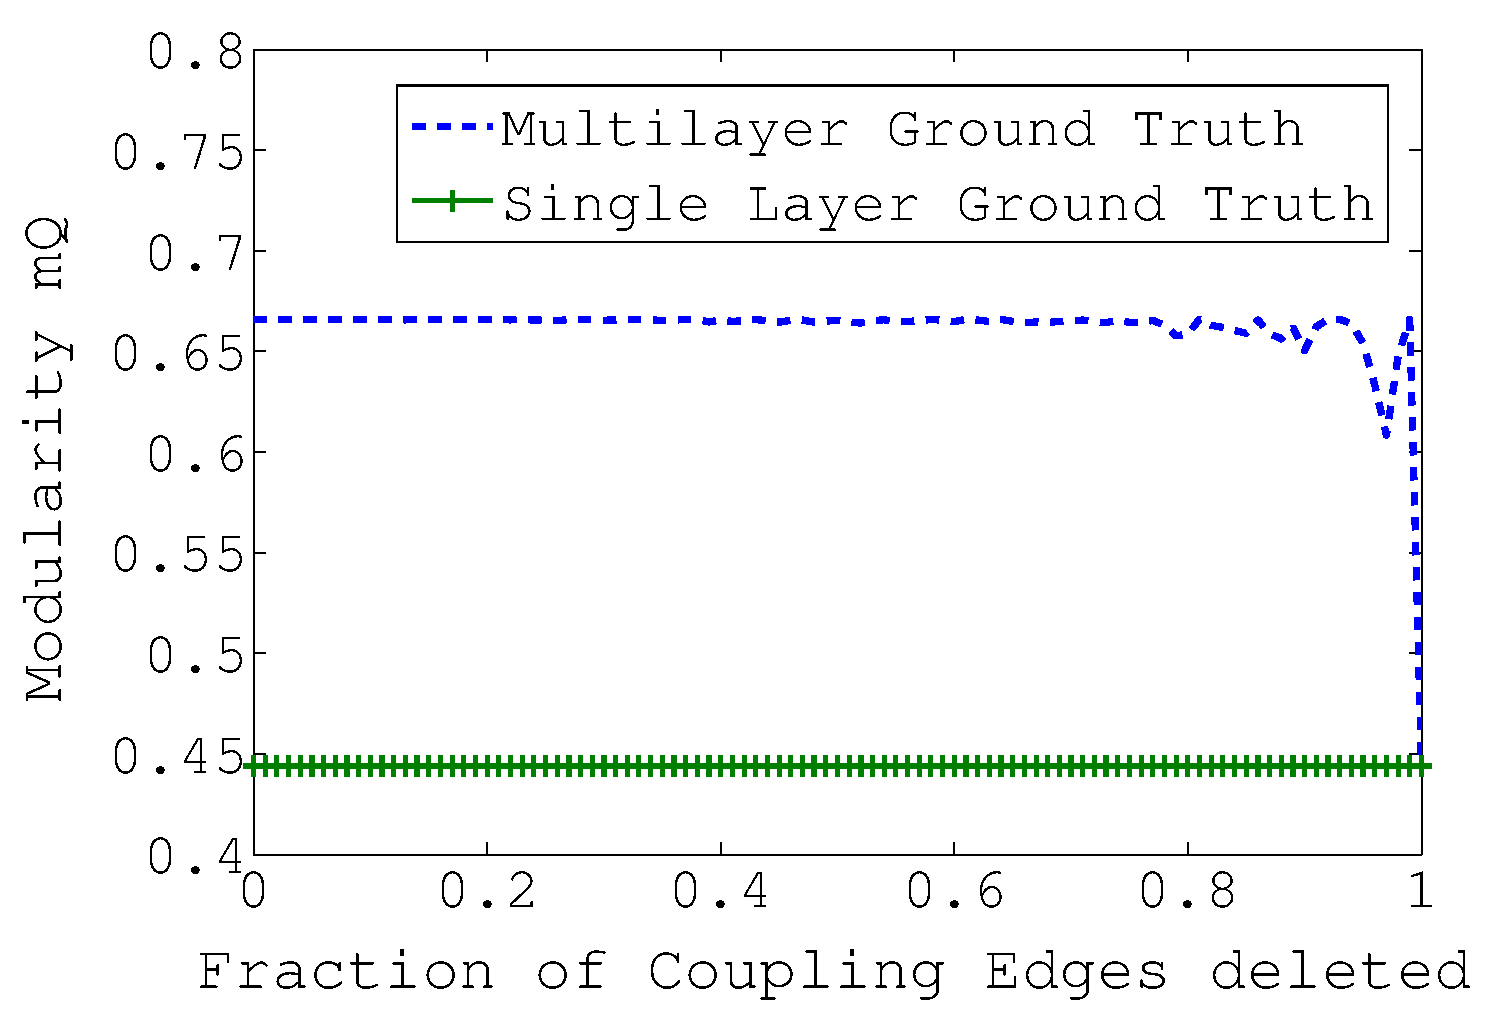
\includegraphics[width=2.5in]{./images/mQ_config1_2_100_5_no_ext_random_removal.pdf}
% % % \vspace{-0.1in}
% % % \caption{Change in mQ while deleting couplinng edges for both ground truth communities in Fig.~\ref{N0}}
% % % \vspace{-0.1in}
% % % \label{mQ1}
% % % \end{figure}
% %
% % \subsubsection{Modularity index $MultiMod$}
% % In order to alleviate the aforesaid limitations of $mQ$, we introduce corrections with each term of it and proposed the following
% % modularity index
% % \begin{dmath}\label{eqn2}
% %  MultiMod=\frac{1}{3}\sum_{C=1}^{n_C}\{[\underbrace{(\frac{\left \vert E^C_1 \right \vert}{\left \vert E_1 \right \vert}-
% %  (\frac{d^C_1}{2\left \vert E_1 \right \vert})^2)}_{Term~ for~ Single~ Layer~ L_1~in~mQ} \times \underbrace{e^{-F^C_1}}_{Correction~ Term}]
% %  +[\underbrace{(\frac{\left \vert E^C_{12} \right \vert}{\left \vert E_{12} \right \vert}-
% %  \frac{k^C_{12}\times{d^C_{12}}}{{\left \vert E_{12} \right \vert}^2})}_{Term~ for~ Coupling~ edges~in~mQ} \times \underbrace{H^C_1\times H^C_2}_{Correction~ Term}]
% %  +[\underbrace{(\frac{\left \vert E^C_2 \right \vert}{\left \vert E_2 \right \vert}-(\frac{d^C_2}{2\left \vert E_2 \right \vert})^2)}_{Term~ for~ Single~ Layer~ L_2~in~mQ}\times \underbrace{e^{-F^C_2}}_{Correction~ Term}]\}
% %  \end{dmath}
% % % \begin{equation}
% % %  mQ=\frac{1}{3}\sum_{c=1}^{n_c}\{\underbrace{[\frac{\left \vert E^C_1 \right \vert}{\left \vert E_1 \right \vert}-
% % %  (\frac{d^C_1}{2\left \vert E_1 \right \vert})^2]}
% % %  +\underbrace{[\frac{\left \vert E^C_{12} \right \vert}{\left \vert E_{12} \right \vert}-
% % %  \frac{k^C_{12}\times{d^C_{12}}}{{\left \vert E_{12} \right \vert}^2}]}
% % %  +\underbrace{[\frac{\left \vert E^C_2 \right \vert}{\left \vert E_2 \right \vert}-(\frac{d^C_2}{2\left \vert E_2 \right \vert})^2]}\}
% % %
% % % \end{equation}
% % % \label{eqn2}
% %
% % %\end{dmath}
% % % MultiMod=\frac{1}{3}\sum_{c=1}^{n_c}\{[(\frac{I_{Ac}}{m_A}-(\frac{d_{Ac}}{2m_A})^2)\times e^{-F^C_1}]+
% % %  [\underbrace{(\frac{I_{\pi c}}{m_\pi}-\frac{k_{\pi c}\times{d_{\pi c}}}{{m_\pi}^2})}\times \underbrace{H^C_1\times H^C_2}]+
% % %  [(\frac{I_{Bc}}{m_B}-(\frac{d_{Bc}}{2m_B})^2)\times e^{-F^C_2}]\}
% % \begin{figure*}
% % \begin{center}
% % \subfigure[Config A
% % ]{\label{single1}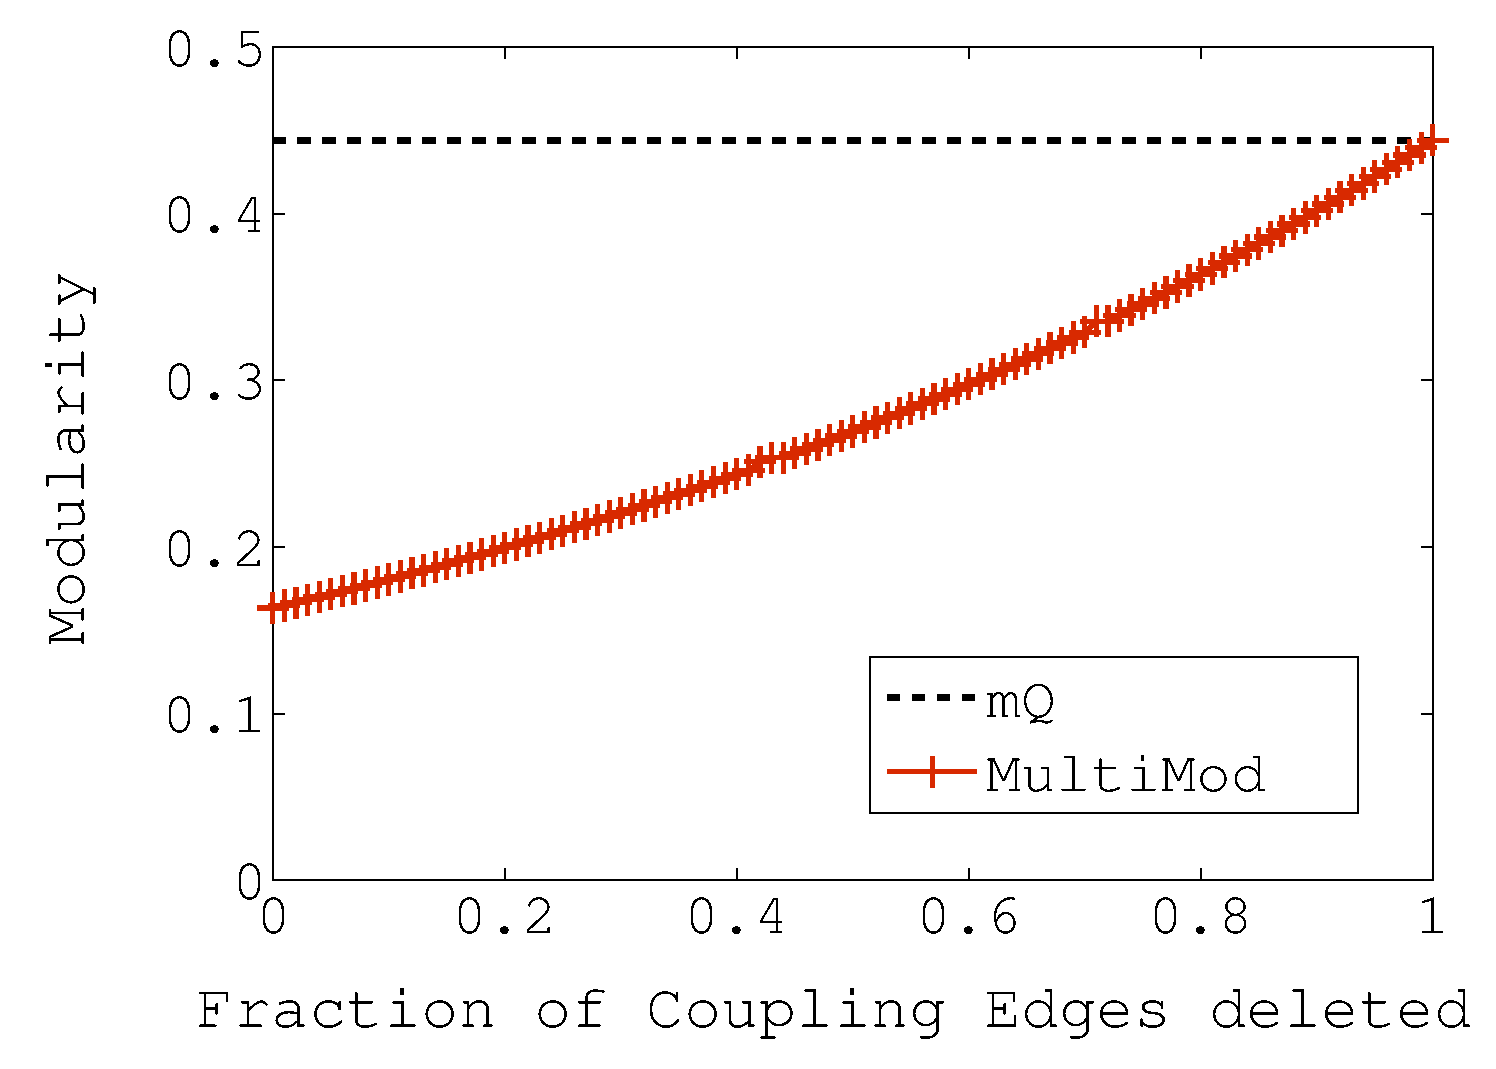
\includegraphics[angle=0,scale=.23]{./images/mQ_vs_single_config2_100_5_no_ext_random_removal.pdf}}
% % \subfigure[Config B
% % ]{\label{single0}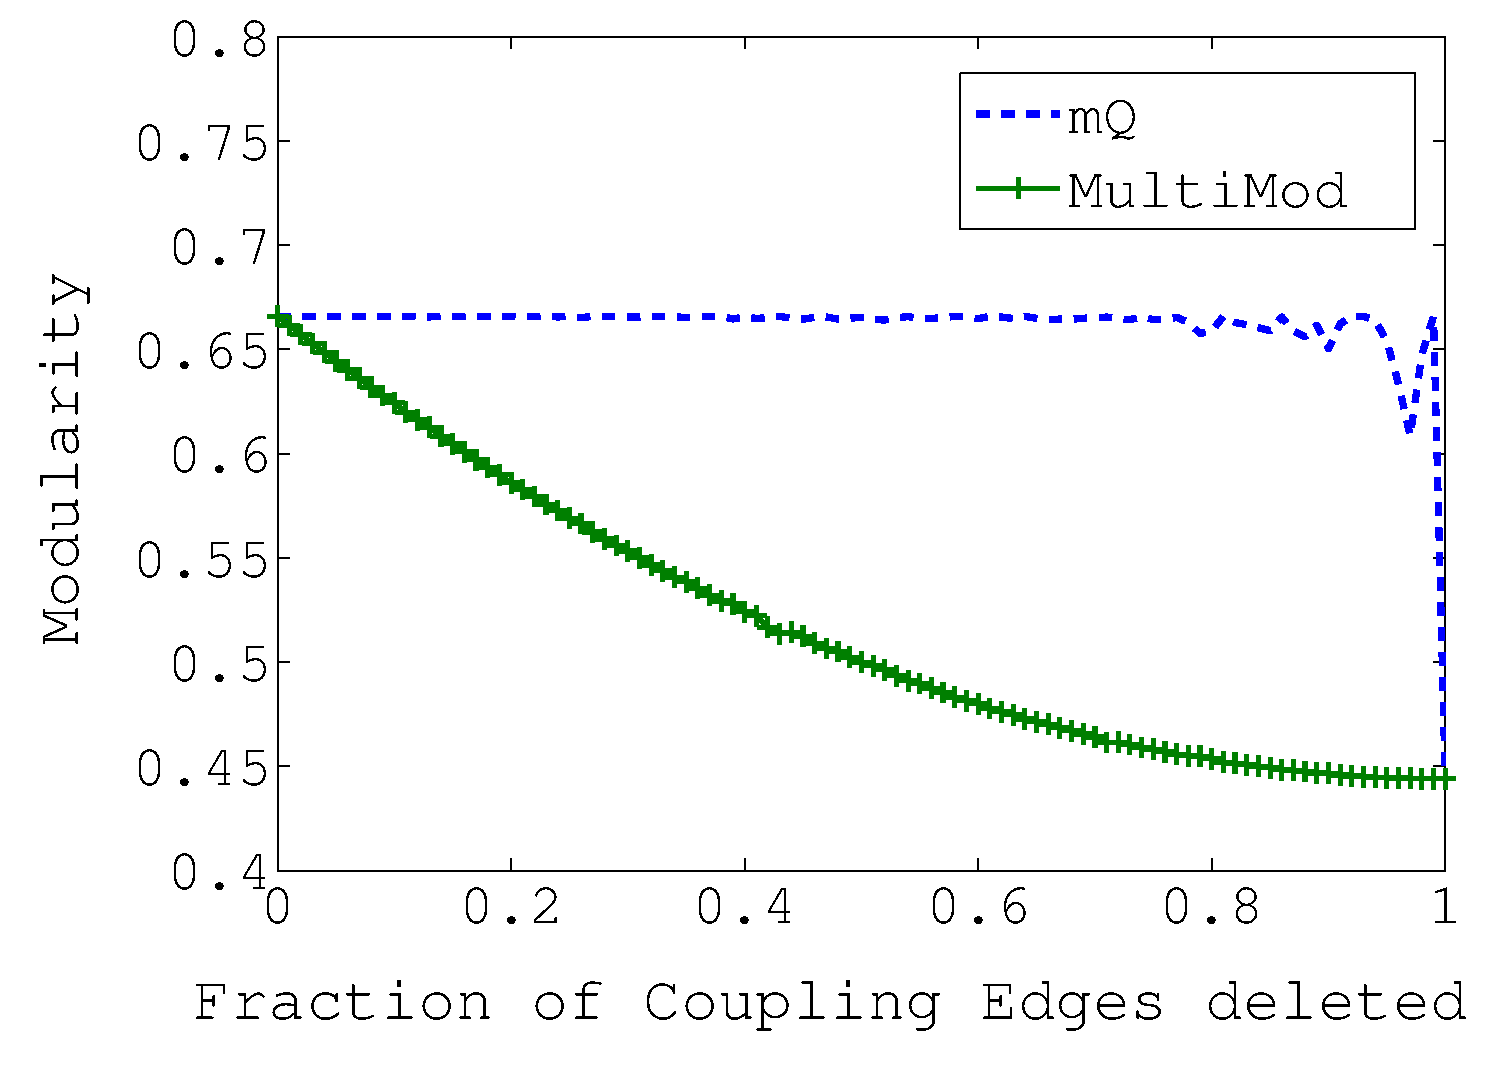
\includegraphics[angle=0,scale=.23]{./images/mQ_vs_single_config1_100_5_no_ext_random_removal.pdf}}
% % \end{center}
% % \vspace{-0.25in}
% % \caption{Change in mQ and MultiMod while deleting coupling edges for both Single layer (Config A) \& Multilayer (Config B) ground truth
% % communities in Fig.~\ref{N0}}
% % \vspace{-0.2in}
% % \label{single}
% % \end{figure*}
% %
% % where $F^C_1$  represents the fraction of $L^C_1$ nodes connected to at least one $L_2$ node from a different community;
% % $H^C_1$ represents the fraction of $L^C_1$ nodes connected to at least one node from $L^C_2$;
% % $F^C_2$ and $H^C_2$ are also defined in the same manner. We summarize the corrections next.
% %
% % (a) We introduce the factors $e^{-F^C_1}$ and $e^{-F^C_2}$, respectively with the corresponding single layer modularity terms.
% % Consider a community $L^C_1$ which is very cohesive in the $L_1$ layer itself, however a high fraction of
% % nodes in $L^C_1$ may also be connected with the nodes of some different community of layer $L_2$ through coupling
% % edges (high $F^C_1$); this should dilute the cohesiveness of community $L^C_1$ and penalize the overall modularity.
% % Hence, we introduce the factors $e^{-F^C_1}$ and $e^{-F^C_2}$ to penalize the single layer terms of modularity.
% % Fig.~\ref{single1} depicts that in Config A, modularity
% % $MultiMod$ gracefully improves as a result of removal of these type of coupling edges.
% %
% % (b) The factor $H^C_1\times H^C_2$, introduced with the coupling layer term of Eq.~\ref{eqn2}, measures how strongly the coupling
% % edges in community $C$ connect the group of nodes
% % $L^C_1$ and $L^C_2$ respectively. In Config B, even if the cross layer term results in high modularity, removal
% % of coupling edges results in low $H^C_1\times H^C_2$, which in turn reduces $MultiMod$. In Fig.~\ref{single0}, we can
% % observe that in Config B, $MultiMod$ gracefully degrades, following our intuition, with deletion
% % of coupling edges.
\subsection{Community detection algorithm}
We leverage on the single layer community detection algorithms Girvan-Newman~\cite{newman2004finding} \& Louvain~\cite{blondel2008fast}
which detect communities by maximizing Girvan-Newman modularity~\cite{newman2006modularity}.
%For example, in Girvan-Newman algorithm, we partition the network by removing edges in the descending order
%of their betweenness-centrality values and obtain the partition with highest modularity.
%Similar modularity maximization is adopted for Louvain too.

\vspace{-0.1in}
\begin{algorithm} \small

    \DontPrintSemicolon
    \SetKwInOut{Input}{Input}
    \SetKwInOut{Output}{Output}
    \SetKwProg{Fn}{Function}{:}{}
     \Input{A multilayer network $\mathcal{G}$ as defined in section~\ref{mult_mod} where $V= V_1 \cup V_2$.} 
%     is the set of all nodes in all the layers of $\mathcal{G}$.}
     \Output{Maximum $Q_M$ of $\mathcal{G}$ and detected communities.}

%      \ForEach{$node \in N_E \cup N_V$}{%
%       act[node]=0\;
%      }
% % \While{$\left \vert V \right \vert > 0$}{
% %      $oldQ$=-1\;
% %      $currQ$=0\;
% %      $Ite$=0\;
% %      $reassign$=0\;
% %      \While{$oldQ$ $\neq$ $currQ$ and $Ite < MaxIt$}{
% %       $oldQ$=$currQ$\;
% %       $currQ$=0\;
% %       $Ite=Ite+1$\;
% %       \ForEach{$v \in V$}{%
% % 	$currQ$ = current $Q_M$ of $G$\;
% % 	$Nei(v)$ = set of neighboring communities of $v$\;
% % 	
% % 	\ForEach{community $c \in Nei(v)$}{ %\textit{//Neighbours of $e_{max}$ in $X_E$}   \;
% % 	  Put $v$ into $c$\;
% % 	  $newQ$ = current $Q_M$ of $G$\;
% % 	  $gain_c$ = $newQ - currQ$
% % 	}
% % 	$c_{max}$ = Find $c \in Nei(v)$ with maximum $gain_c$\;
% % 	\uIf{$gain_{c_{max}} > 0$}{
% % 	    Assign $v$ to $c_{max}$\;
% % 	    $reassign=1$\;}
% % 	  \Else{
% % 	    Keep $v$ in its current community\;}
% % 	
% %  	
% %  	
% %        }
% %       $currQ$ = current $Q_M$ of $G$
% % }	
% % \If{$reassign==0$}
% %  	{break\;}
% %  $G$= Modify G by considering the detected communities as nodes and updating edges between them accordingly.	
% % }
% %      $currQ$ is the maximized $Q_M$\;

    \While{True}{
      Place each node of $\mathcal{G}$ into a single community\;
      Save $Q_M$ for this decomposition\;
      \While {there are moved nodes}{
	\ForEach{node $n \in V$}{
	    c = neighboring community of $n$ maximizing $Q_M$ increase\;
	    \If{c results in a strictly positive increase}{
	      move n from its community to c\;
	    }
	}
      }
      \uIf {$Q_M$ reached is higher than the initial $Q_M$}{
	Display the partition found\;
	Transform $\mathcal{G}$ into the network between communities\;
	}
      \Else{
	break\;
      }
    }
    \KwRet\;

\caption{Louvain-$Q_M$} %Algorithm to map Meetup venues with Yelp venues}
\label{algo2}
\end{algorithm}
\vspace{-0.1in}


We substitute the Girvan-Newman modularity by our proposed modularity index $Q_M$ and develop \textbf{GN-$Q_M$} (Algo.~\ref{algo3})
and \textbf{Louvain-$Q_M$} (Algo.~\ref{algo2}) algorithms respectively for multilayer networks.
Although vanilla algorithms are intrinsically incapable of distinguishing different types of edges and nodes in the multilayer 
network, however, due to
the adaptability of $Q_M$, \textbf{GN-$Q_M$} and \textbf{Louvain-$Q_M$} should be able to detect both cross layer
and single layer communities. Essentially $Q_M$ works as a patch on top of any single layer
community detection algorithm to detect multilayer communities.

% \begin{itemize}
%  \item \textbf{GN-$Q_M$}: In this algorithm (see Alg.~\ref{algo3}), at every step we remove an edge with the maximum
%  betweenness centrality until there are no edges left in the graph. During this process, we save the $Q_M$
%  value corresponding to each partition created after the edge removal and finally output the partition with the maximum $Q_M$ value.


% %  \item \textbf{Louvain-$Q_M$}: In this algorithm (see Algo.~\ref{algo2}), we begin with initializing
% % every node of the input network to a singleton community. A node is moved to a neighbouring community only if this movement results in a
% % strictly positive increase in $Q_M$ of the entire network. This process is repeated for each vertex and the iteration ends when no
% % other movement is possible. At the next pass, all the detected communities are considered as nodes (edges updated accordingly) and the
% % same process continues. The algorithm stops if there is no increase in $Q_M$ value in a particular pass and thereby, the most recent
% % partition is obtained as the output of the algorithm.
% % \end{itemize}

%
% Our algorithm is a heuristic, that strives to obtain a high value of $Q_M$. In this algorithm, we begin with initializing
% every vertex to a singleton community. A vertex is moved to a community only if this movement results in a
% net increase in $Q_M$ of the entire network.
% This process is repeated for each vertex and the iteration ends when no other movement is possible.
% At the next step all the detected communities are considered as vertices (edges updated accordingly) and the
% same process continues.
% This process is repeated for each vertex and the entire relocation of
% all vertices is repeated over several iterations until the $Q_M$ value converges.
% However, convergence is not theoretically guaranteed, but we empirically observe that the algorithm
% converges with high probability.

\subsection{Convergence \& Complexity}
Finally we show that algorithms \textbf{GN-$Q_M$} and \textbf{Louvain-$Q_M$}
converge and they are tractable in terms of time complexity.

\subsubsection{\textbf{GN-$Q_M$}} At every step we remove one edge from the network and hence, the algorithm certainly stops
after the removal of all the $\left \vert E_1 \right \vert + \left \vert E_{12} \right \vert+ \left \vert E_2 \right \vert$ edges.
Clearly, the theoretical worst case complexity of the algorithm is
$O((\left \vert V_1 \right \vert + \left \vert V_2 \right \vert)\times(\left \vert E_1 \right \vert +
\left \vert E_{12} \right \vert+ \left \vert E_2 \right \vert)^2)$ as finding betweenness centrality in unweighted graphs
costs $O((\left \vert V_1 \right \vert + \left \vert V_2 \right \vert)\times(\left \vert E_1 \right \vert +
\left \vert E_{12} \right \vert+ \left \vert E_2 \right \vert))$ operations~\cite{PhysRevE.64.016132}.
%\textcolor{red}{[SP:Please check. Ref needed?, JLG: Ok, ref is Newman M E J(2001) Phys Rev E 64:016131]}



\subsubsection{\textbf{Louvain-$Q_M$}} At each iteration of every pass, each node is placed
into one of its neighbouring community only if the movement leads to a
strictly positive gain in modularity $Q_M$. Computing this gain both proves
that the algorithms converges and gives an upper bound on its complexity.

Suppose, at any particular iteration the node $x$ is to be moved from its own
community $C_1$ to another community $C_2$. Without loss of generality, let us
assume that $x \in V_1$ and $x$ is connected with $h_x$ nodes in $V_1$ \& $c_x$
nodes in $V_2$. For simplicity, we perform this movement in two steps: first, we
remove $x$ from $C_1$ and keep it as an isolated community; second,
we insert $x$ into $C_2$. $C_1$ and $C_2$ can be either cross layer or
single layer communities, independently. Below we derive the gain assuming
$C_1$ is cross layer and $C_2$ is single layer. The other three cases can be
derived in a similar manner. Note that since the
modularity is an independent sum over all communities, the contribution of other communities
than $C_1$ and $C_2$ is not affected by the movement of $x$. Therefore we will only compute
the change of modularity of $C_1$ and $C_2$.

%This makes our approach heavily generic and flexible.
%In the next section, we compare the performance of our algorithm with different types of existing baseline algorithms.


%Similar to Eq.~\ref{final1},
The modularity $Q_M^{C_1,C_2}$, restricted to $C_1$ and $C_2$, before any movement can be simply expressed as,
$Q_M^{C_1,C_2} = Q_M^{C_1}+ Q_M^{C_2}$,
where $Q_M^{C_1}$ follows from Eq.~\ref{eq_multi} (as $C_1$ is cross layer) and $Q_M^{C_2}$ follows from Eq.~\ref{eq_single}
(as $C_2$ is single layer).
%\begin{dmath}\label{final2}
%Q_M= \frac{1}{3}\left[ {\forall i,j \in C_1}~\penalty0   \bigg \{
% \frac{1}{2\left \vert E_1 \right \vert }
% \sum_{i,j \in V_1}(A_{ij} - \penalty0 \frac{ (h_i * h_j)}
% {2\left \vert E_1 \right \vert})  \\
% +
% \frac{1}{2\left \vert E_1 \right \vert + 2\left \vert E_2 \right \vert + \left \vert E_{12} \right \vert} \penalty0
% \sum_{i \in V_1, j \in V_2}(A_{ij} - \frac{ ({c'}_i * {c'}_j)}
% {2\left \vert E_1 \right \vert + 2\left \vert E_2 \right \vert + \left \vert E_{12} \right \vert}) \\+
% \frac{1}{2\left \vert E_{2} \right \vert} \penalty0
% \sum_{i,j \in V_2}(A_{ij} -
% \frac{ (h_i * h_j)}{2\left \vert E_2 \right \vert })
%   \bigg \} \right] +
%\frac{1}{3}\left[ {\forall i,j \in C_2}~\penalty0   \bigg \{
% \frac{1}{2\left \vert E_1 \right \vert + \left \vert E_{12} \right \vert }
% \sum_{i,j \in V_1}(A_{ij} - \penalty0 \frac{ (h_i+c_i) * (h_j+c_j)}
% {2\left \vert E_1 \right \vert+ \left \vert E_{12} \right \vert})
%   \bigg \} \right] +   \frac{1}{3}\sum_{k=3}^{n_C} Q_M^{C_k}
%\end{dmath}

% % \begin{dmath}\label{final2}
% % %Q_M= \frac{1}{3}\left[ {\forall i,j \in C_1}~\penalty0   \bigg \{
% % % \frac{1}{2\left \vert E_1 \right \vert }
% % % \sum_{i,j \in V_1}(A_{ij} - \penalty0 \frac{ (h_i * h_j)}
% % % {2\left \vert E_1 \right \vert})  \\
% % % +
% % % \frac{1}{2\left \vert E_1 \right \vert + 2\left \vert E_2 \right \vert + \left \vert E_{12} \right \vert} \penalty0
% % % \sum_{i \in V_1, j \in V_2}(A_{ij} - \frac{ ({c'}_i * {c'}_j)}
% % % {2\left \vert E_1 \right \vert + 2\left \vert E_2 \right \vert + \left \vert E_{12} \right \vert}) \\+
% % % \frac{1}{2\left \vert E_{2} \right \vert} \penalty0
% % % \sum_{i,j \in V_2}(A_{ij} -
% % % \frac{ (h_i * h_j)}{2\left \vert E_2 \right \vert })
% % %   \bigg \} \right] +
% % %\frac{1}{3}\left[ {\forall i,j \in C_2}~\penalty0   \bigg \{
% % % \frac{1}{2\left \vert E_1 \right \vert + \left \vert E_{12} \right \vert }
% % % \sum_{i,j \in V_1}(A_{ij} - \penalty0 \frac{ (h_i+c_i) * (h_j+c_j)}
% % % {2\left \vert E_1 \right \vert+ \left \vert E_{12} \right \vert})
% % %   \bigg \} \right] +   \frac{1}{3}\sum_{k=3}^{n_C} Q_M^{C_k}
% % Q_M^{C_1,C_2}= \frac{1}{3}\left[
% %  \frac{1}{m_1} \sum_{i,j \in V_1,C_1} ( A_{ij} - \penalty0 \frac{h_i h_j}{m_1} ) +  \\
% %   \frac{1}{m} \penalty0
% %  \sum_{i \in V_1, j \in V_2, C_1}(A_{ij} - \frac{{c'}_i {c'}_j}{m}) +
% %  \frac{1}{m_2} \sum_{i,j \in V_2,C_1}(A_{ij} - \frac{h_i h_j}{m_2})
% %    \right] +\penalty0
% % \frac{1}{3}\left[
% %  \frac{1}{m_{12}} \sum_{i,j \in V_1,C_2}(A_{ij} - \frac{(h_i+c_i) (h_j+c_j)}{m_{12}})
% %   \right]
% % \end{dmath}

Once node $x$ is removed from $C_1$ and kept as an isolated community, the modularity sum of the $C_1$, $C_2$ and ${x}$ becomes,
%\textcolor{red}{[JL: Can you make the $+1/m$ from en of first line of the equation to go on the second line?]}
\vspace{-0.18in}
\begin{dmath*}\label{final3}
Q_M^{C_1,C_2,\{x\}}= \frac{1}{3}\left[
 \frac{1}{m_1} \sum_{i,j \in V_1 ,C_1 - \{x\}} \big(A_{ij} - \penalty0 \frac{h_i h_j}{m_1}\big) +\\
 {\frac{1}{m}  \sum_{i,j \in  C_1 - \{x\}, i \in V_1, j \in V_2} \big(A_{ij} - \frac{ {c'}_i {c'}_j}{m}\big) +
 \frac{1}{m_2}} \penalty0 \sum_{i,j \in V_2,C_1 - \{x\}} \big(A_{ij} - \frac{h_i h_j}{m_2}\big) \right] +  
 \frac{1}{3}\left[ \frac{1}{m_{21}} \penalty0 \big(A_{xx} - \frac{(h_x+c_x)^2}{m_{21}}\big)\right] + Q_M^{C_2}
 %\frac{1}{3}\left[ \frac{1}{m_{12}} \sum_{i,j \in V_1,C_2} (A_{ij} - \frac{(h_i+c_i)(h_j+c_j)}{m_{12}}) \right]
\end{dmath*}
\vspace{-0.05in}
where $m_1=2\left \vert E_1 \right \vert$, $m_2=2\left \vert E_2 \right \vert$,
$m_{12} = 2\left \vert E_1 \right \vert + \left \vert E_{12} \right \vert$, $m_{21} = 2\left \vert E_2 \right \vert + \left \vert E_{12} \right \vert$ and
$m=2\left \vert E_1 \right \vert + 2\left \vert E_2 \right \vert + \left \vert E_{12} \right \vert$.

Hence, the change in modularity $\Delta_r=Q_M^{C_1,C_2,\{x\}}-Q_M^{C_1,C_2}$ due to this removal (assuming $A_{xx} = 0$) is the following,
\vspace{-0.05in}
\begin{dmath*}\label{final4}
\Delta_r = \frac{h_x^2}{3{m_1}^2} -
  \frac{1}{3}\left[
    \frac{1}{m_1} \sum_{i \in V_1, C_1 - \{x\}} \big(A_{ix} - \frac{(h_i h_x)}{m_1}\big) +
    \frac{1}{m} \sum_{i \in V_2, C_1 - \{x\}} \big(A_{xi} - \frac{ {c'}_x  {c'}_i}{m}\big)
    \right] - \frac{ (h_x+c_x)^2}{3m_{21}^2}
% \Delta_{removal} = Q_M^{'}-Q_M = -
%\frac{1}{3}\left[ {\forall i \in C_1 - \{x\}}~\penalty0   \bigg \{
% \frac{1}{2\left \vert E_1 \right \vert }
% \sum_{i \in V_1}(A_{ix} - \penalty0 \frac{ (h_i * h_x)}
% {2\left \vert E_1 \right \vert})  \\
% +
% \frac{1}{2\left \vert E_1 \right \vert + 2\left \vert E_2 \right \vert + \left \vert E_{12} \right \vert} \penalty0
% \sum_{i \in V_2}(A_{xi} - \frac{ ({c'}_x * {c'}_i)}
% {2\left \vert E_1 \right \vert + 2\left \vert E_2 \right \vert + \left \vert E_{12} \right \vert})\bigg \} \right] -
%  \frac{1}{3}\left[
% \frac{ (h_x+c_x)^2}{(2\left \vert E_2 \right \vert + \left \vert E_{12} \right \vert)^2}\right]
% + \frac{h_x^2}{3.(2\left \vert E_1 \right \vert)^2}
\end{dmath*}
\vspace{-0.05in}

%After inserting $x$ into $C_2$, $Q_M$ can be expressed as,
%\begin{dmath}\label{final5}
%Q_M^{''}= \frac{1}{3}\left[ {\forall i,j \in C_1 - \{x\}}~\penalty0   \bigg \{
% \frac{1}{2\left \vert E_1 \right \vert }
% \sum_{i,j \in V_1}(A_{ij} - \penalty0 \frac{ (h_i * h_j)}
% {2\left \vert E_1 \right \vert})  \\
% +
% \frac{1}{2\left \vert E_1 \right \vert + 2\left \vert E_2 \right \vert + \left \vert E_{12} \right \vert} \penalty0
% \sum_{i \in V_1, j \in V_2}(A_{ij} - \frac{ ({c'}_i * {c'}_j)}
% {2\left \vert E_1 \right \vert + 2\left \vert E_2 \right \vert + \left \vert E_{12} \right \vert}) +
% \frac{1}{2\left \vert E_{2} \right \vert} \penalty0
% \sum_{i,j \in V_2}(A_{ij} -
% \frac{ (h_i * h_j)}{2\left \vert E_2 \right \vert })
%   \bigg \} \right] +
%\frac{1}{3}\left[ {\forall i,j \in C_2+\{x\}}~\penalty0   \bigg \{
% \frac{1}{2\left \vert E_1 \right \vert + \left \vert E_{12} \right \vert }
% \sum_{i,j \in V_1}(A_{ij} - \penalty0 \frac{ (h_i+c_i) * (h_j+c_j)}
% {2\left \vert E_1 \right \vert+ \left \vert E_{12} \right \vert})
%   \bigg \} \right]
% +  \frac{1}{3}\sum_{k=3}^{n_C} Q_M^{C_k}
%\end{dmath}

Similarly, the change in modularity $\Delta_i$ due to the insertion of $x$ in
$C_2$ can be computed as,
\vspace{-0.05in}
\begin{dmath*}\label{final6}
\Delta_{i} =
 \frac{1}{3m_{12}}
 \sum_{i \in V_1, C_2}\big(A_{ix} - \frac{ (h_i+c_i)(h_x+c_x)}{m_{12}}\big)+\frac{ (h_x+c_x)^2}{3m_{21}^2}
\end{dmath*}
\vspace{-0.05in}
Finally, the overall improvement due to this movement of node $x$ from
community $C_1$ to community $C_2$ is\footnote{Same order of magnitude can
be derived for other types of $C_1$ and $C_2$.},
\vspace{-0.05in}
\begin{dmath*}\label{final7}
\Delta_{r}+\Delta_{i} = \Theta(\frac{1}{m^2})
% Q_M^{''}-Q_M =
%\Delta_{removal}+\Delta_{insertion} = -
%\frac{1}{3}\left[ {\forall i \in C_1 - \{x\}}~\penalty0   \bigg \{
% \frac{1}{2\left \vert E_1 \right \vert }
% \sum_{i \in V_1}(A_{ix} - \penalty0 \frac{ (h_i * h_x)}
% {2\left \vert E_1 \right \vert})  \\
% +
% \frac{1}{2\left \vert E_1 \right \vert + 2\left \vert E_2 \right \vert + \left \vert E_{12} \right \vert} \penalty0
% \sum_{i \in V_2}(A_{xi} - \frac{ ({c'}_x * {c'}_i)}
% {2\left \vert E_1 \right \vert + 2\left \vert E_2 \right \vert + \left \vert E_{12} \right \vert})\bigg \} \right]
% + \frac{h_x^2}{3.(2\left \vert E_1 \right \vert)^2} +\frac{1}{3}\left[ {\forall i \in C_2}~\penalty0   \bigg \{
% \frac{1}{2\left \vert E_1 \right \vert + \left \vert E_{12} \right \vert }
% \sum_{i \in V_1}(A_{ix} - \penalty0 \frac{ (h_i+c_i) * (h_x+c_x)}
% {2\left \vert E_1 \right \vert+ \left \vert E_{12} \right \vert})
%   \bigg \} \right]
%   \geq \frac{1}{({2\left \vert E_1 \right \vert + 2\left \vert E_2 \right \vert +
%\left \vert E_{12} \right \vert})^2}
\end{dmath*}
\vspace{-0.05in}

Since the minimum gain for every move is of the order of $1/m^2$, in the worst
case we need $O(m^2)$ iterations to maximize $Q_M$ (as it is comprised between -1 and 1).
%As each iteration considers every vertex once, it leads to
%$O({\left \vert V_1 \right \vert + \left \vert V_2 \right \vert})$ operations
%per iteration. The theoretical worst case complexity of \textbf{Louvain-$Q_M$}  is therefore
%$O(({\left \vert V_1 \right \vert + \left \vert V_2 \right \vert})m^2)$.
%\textcolor{red}{[JL: we forgot the cost for computing the best neighboring community, we can cite Louvain directly or the below paper]}
We apply the same technique as in~\cite{blondel2008fast} to find the best neighboring community, so the cost for one vertex
is proportional to its degree. As each iteration considers every vertex once, it leads to $O(m)$ operations per iteration. The
theoretical worst case complexity of \textbf{Louvain-$Q_M$} is therefore $O(m^3)$.
In practice, this worst case complexity bound is quite loose. For instance, in
Fig.~\ref{gain}, we show the fraction of nodes moved along with the gain in
modularity in each iteration of the first pass of the \textbf{Louvain-$Q_M$} algorithm
while running it on a synthetic two layer network (generated following section~\ref{syn_gen}). The network has $600$ nodes ($300$ in
each layer) with $29,738$ edges ($m^2 = 1,104,232,900$) and the theoretical number of iterations could be of the
order 1 billion but it takes just $5$ iterations to end the first pass.

% \begin{figure}
% \centering
% 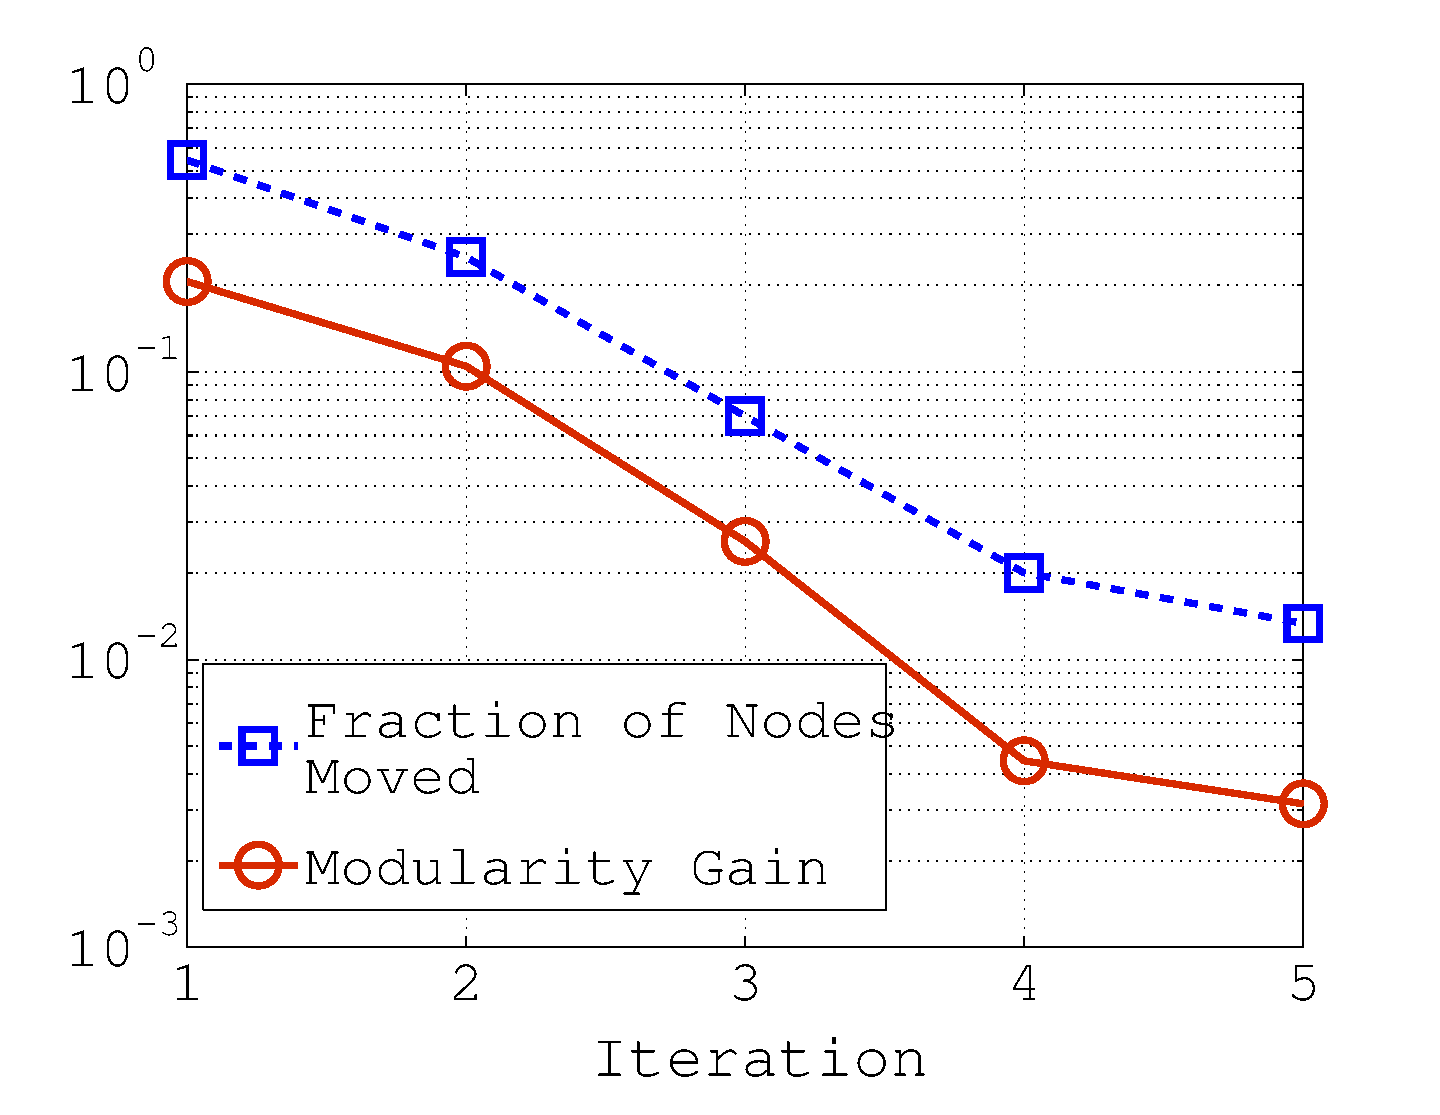
\includegraphics[width=2in]{./images/gain_drop.pdf}
% \vspace{-0.12in}
% \caption{Drop in modularity gain along with fraction of modes moved in the first pass of \textbf{Louvain-$Q_M$} for a $300\times300$
% synthetic multilayer network.}
% \vspace{-0.15in}
% \label{gain}
% \end{figure}


\begin{figure*}
\begin{center}
\subfigure[Drop in modularity gain with number of iterations.
]{\label{gain}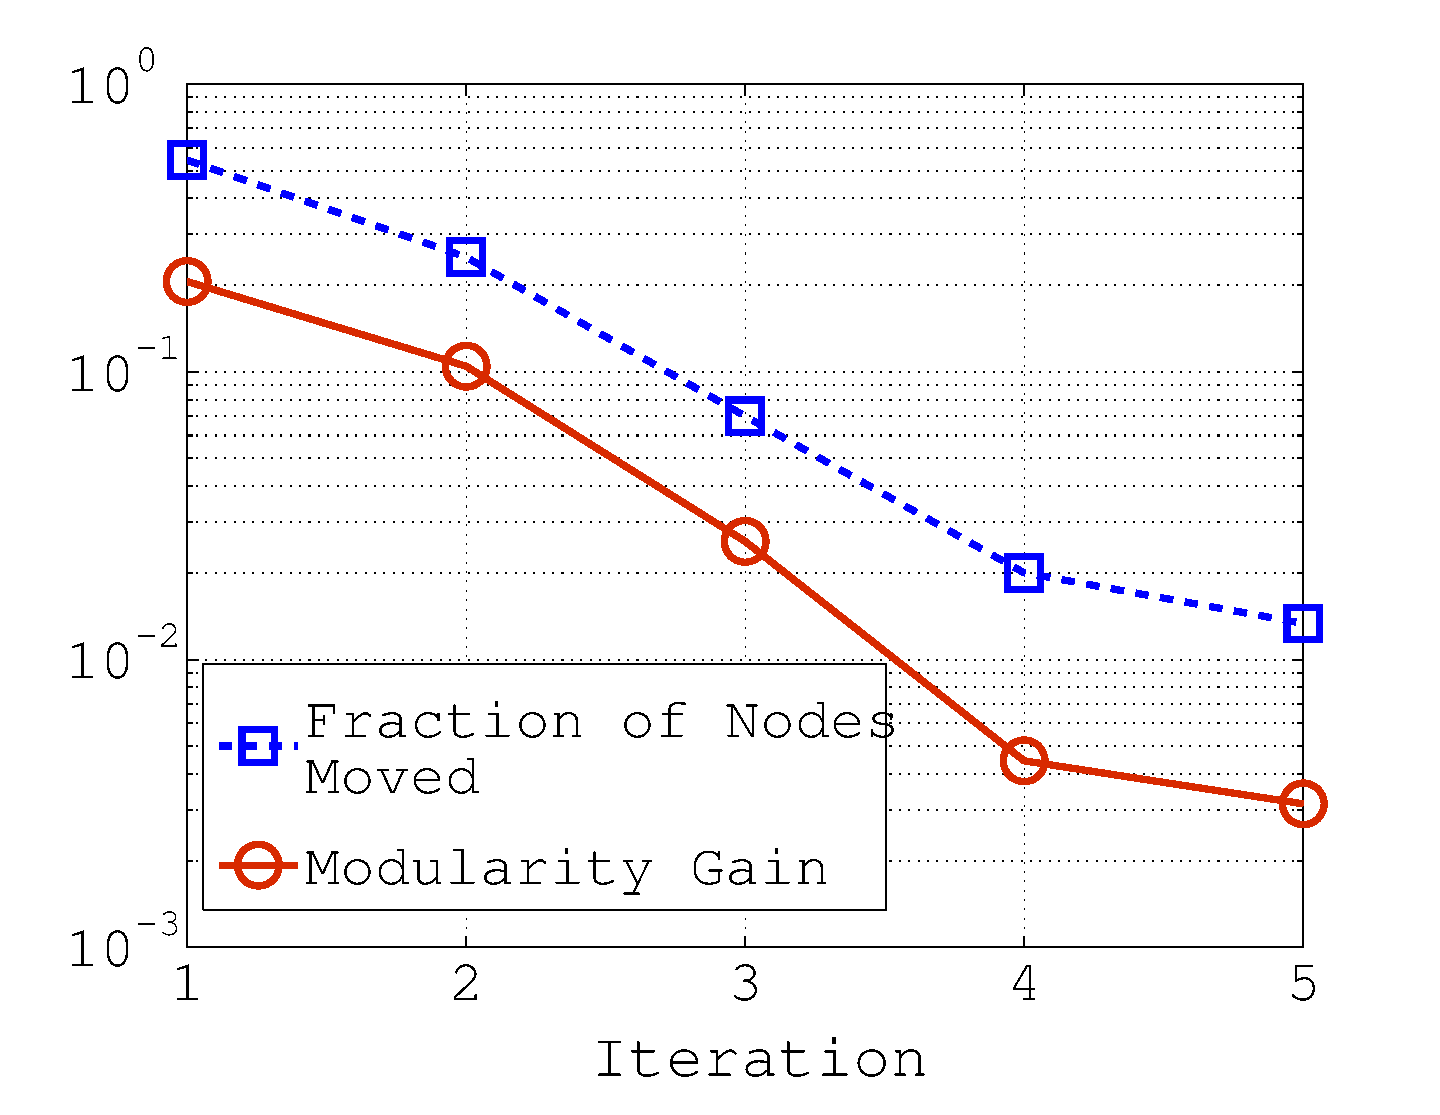
\includegraphics[angle=0,scale=.18]{./images/gain_drop.pdf}}
\subfigure[$mQ$ vs. $Q_M$ for Config A while adding coupling links.
]{\label{cross_single}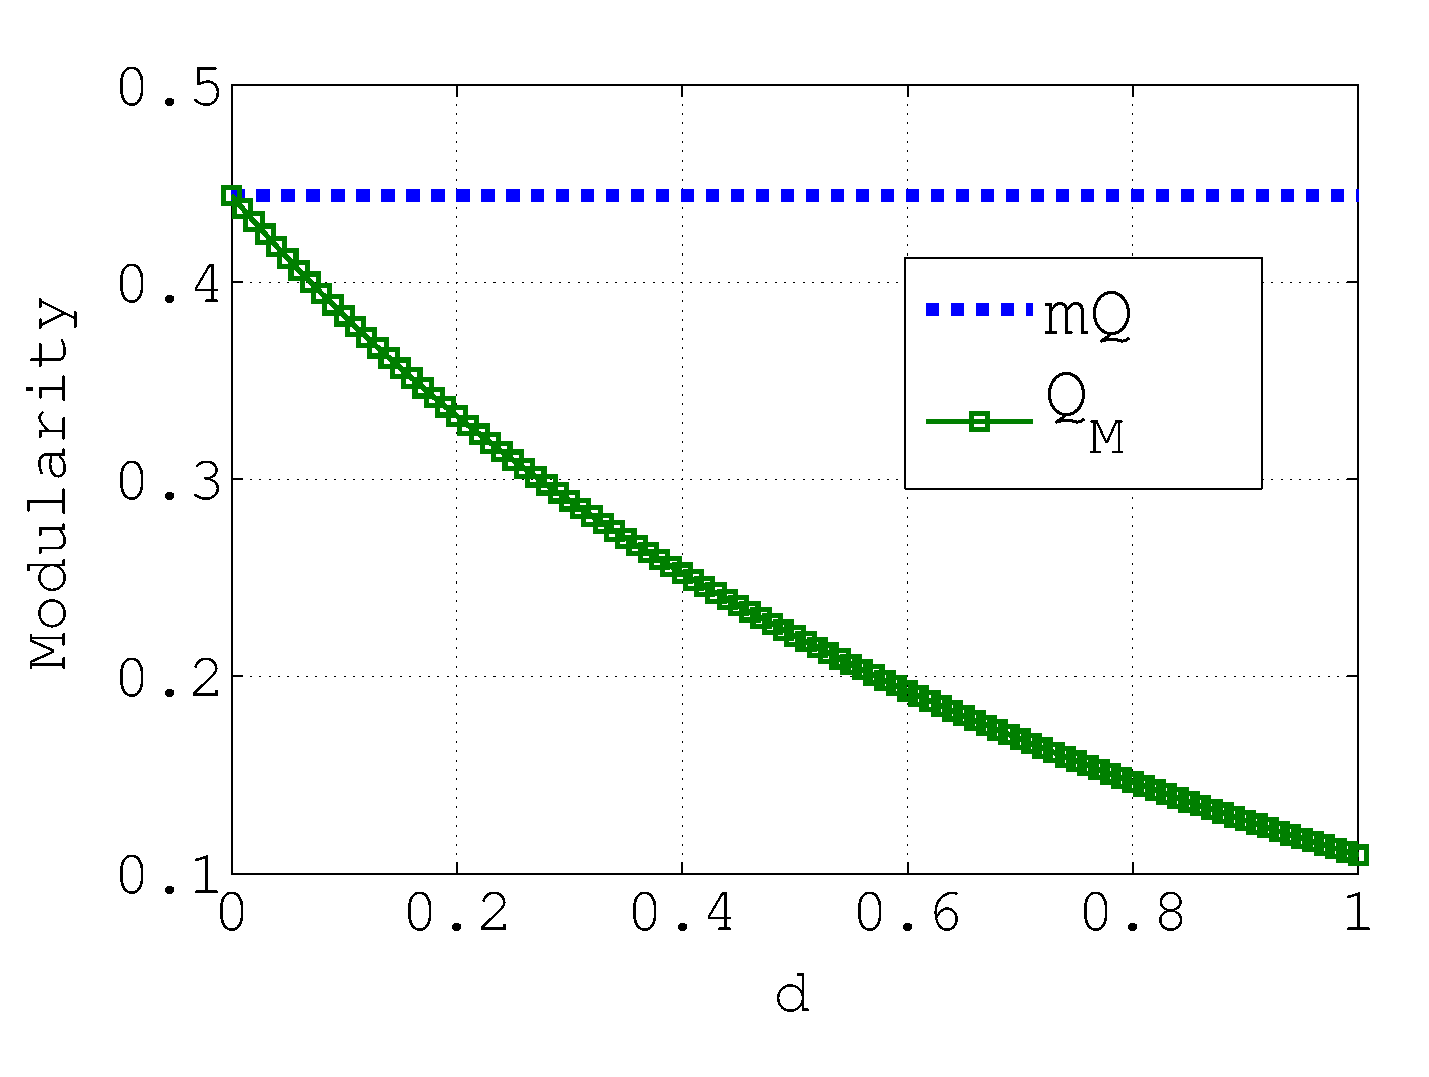
\includegraphics[angle=0,scale=.18]{./images/mQ_vs_march21_cross_single_square.pdf}}
\subfigure[$mQ$ vs. $Q_M$ for Config B while adding coupling links with varying $p$.
]{\label{cross_multi}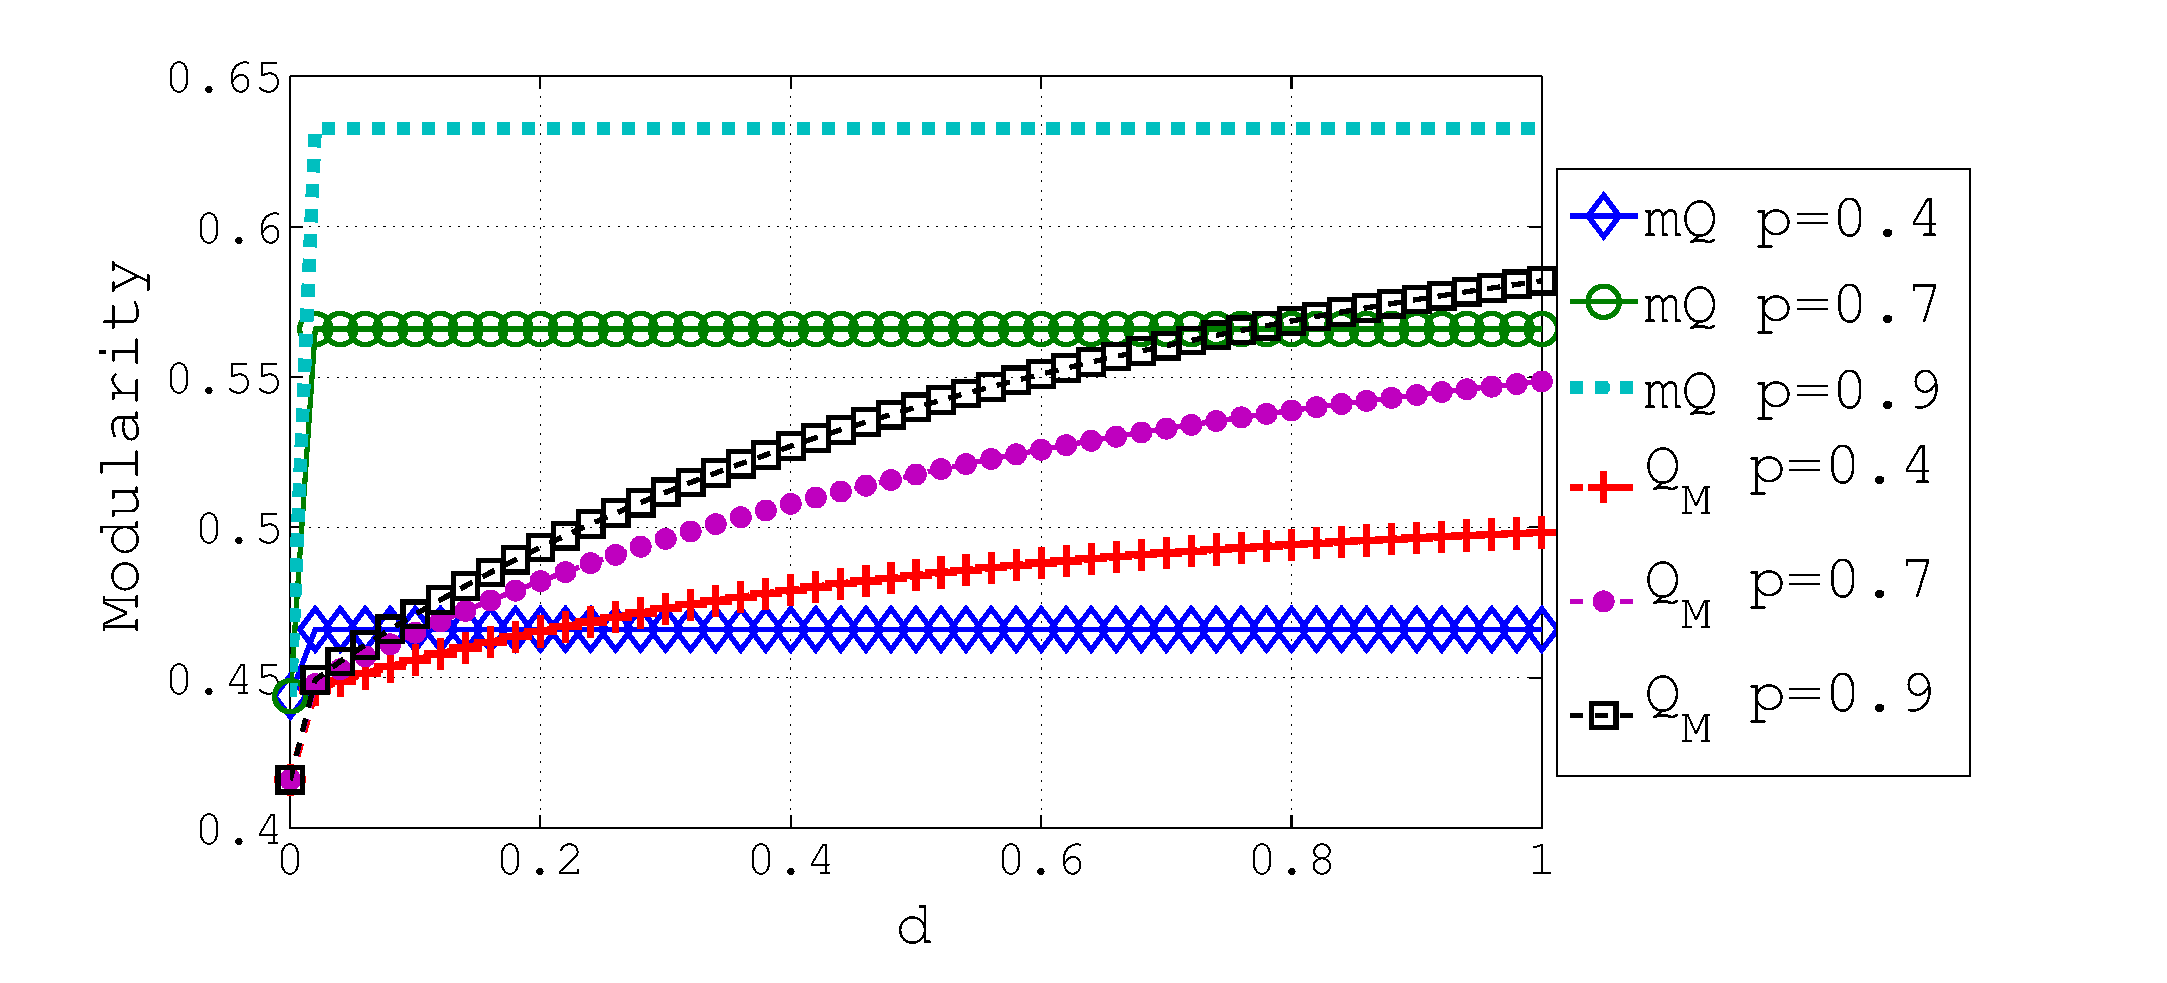
\includegraphics[angle=0,scale=.18]{./images/mQ_vs_march21_cross_multi.pdf}}
\end{center}
\vspace{-0.24in}
\caption{(a) Drop in modularity gain along with fraction of modes moved in the first pass of \textbf{Louvain-$Q_M$} for a $300\times300$
synthetic multilayer network; (b) \& (c) Comparative results
of $Q_M$ \& $mQ$ on the configurations in Fig.~\ref{N0}.}
\vspace{-0.22in}
\label{cross_multi_single}
\end{figure*}


\section{Evaluation: Modularity Index $Q_M$}\label{ev_metric}
In this section, we evaluate the proposed multilayer modularity $Q_M$ against baseline indices. In this experiment, we implement
different configurations of multilayer network following section~\ref{syn_gen} and regulate the tuning parameters to obtain
the desired topology.

\subsection{Baseline Multilayer Modularities}
In literature, very few modularity indices are proposed for multilayer networks, illustrated in~\cite{CompMod} \& \cite{medical_paper}.
Out of this two, `CompMod' proposed in~\cite{CompMod}
works only for communities with single type of nodes (i.e. single layer communities), leaving us with only the modularity `mQ' proposed
in~\cite{medical_paper} to compare with $Q_M$.
For a two-layer network $\mathcal{G} = \{\{L_1, L_2\}, \{L_{12}\}\}$ where $L_1$ = ($V_1$, $E_1$) \& $L_2$ = ($V_2$, $E_2$) are the
individual layers and $L_{12}$ = ($V_1$, $V_2$, $E_{12}$) is the bipartite graph connecting nodes of layer $L_1$ and $L_2$,
$mQ$ can be defined as, %[BM: correct C in the eq.]
\vspace{-0.1in}
\begin{dmath}\label{eq_mQ}
%\resizebox{\columnwidth}{!}{
 {mQ=\frac{1}{3}\sum_{k=1}^{n_C} \bigg \{
 \underbrace{\big(\frac{\left \vert E^{C_k}_1 \right \vert}{\left \vert E_1 \right \vert}-
 (\frac{h^{C_k}_1}{2\left \vert E_1 \right \vert})^2\big)}_{Term~ for~ Single~ Layer~ L_1}}
 +{\underbrace{\big(\frac{\left \vert E^{C_k}_{12} \right \vert}{\left \vert E_{12} \right \vert}-
 \frac{r^{C_k}_{12}*{s^{C_k}_{12}}}{{\left \vert E_{12} \right \vert}^2}\big)}_{Term~ for~ Coupling~ Edges}
 +\underbrace{\big(\frac{\left \vert E^{C_k}_2 \right \vert}{\left \vert E_2 \right \vert}-(\frac{h^{C_k}_2}{2\left \vert
 E_2 \right \vert})^2\big)}_{Term~ for~ Single~ Layer~ L_2} \bigg\}}
 %}
\end{dmath}
\vspace{-0.1in}
%[BM: with underbrace, write - term for single layer $L_1$, term for crosslayer edges, term for single layer $L_2$]
where each community ${C_k}$ 
%[BM: make suitable changes in notation here] 
is represented as $\{\{L^{C_k}_1, L^{C_k}_2\}, 
\{L^{C_k}_{12}\}\}$;
$L^{C_k}_1$ and $L^{C_k}_2$ are the submodules with $E^{C_k}_1$ \& $E^{C_k}_2$ edges from $E_1$ and $E_2$ respectively
whereas $L^{C_k}_{12}$ contains $E^{C_k}_{12}$ edges from $E_{12}$;
%$I^C_1$ is the number of edges in submodule $L^C_1$ i.e. $I^C_1 = \left \vert E^C_1 \right \vert$,
%$m_1$ is the size of subnetwork $G_1$ i.e. ,
$n_C$ is the number of apriori communities; $h^{C_k}_i$ is the sum of degrees of all $L^{C_k}_i$ nodes in $L_i$ layer;
$r^{C_k}_{12}$ is the sum of degrees of $L^{C_k}_1$ nodes in subnetwork $L_{12}$ and $s^{C_k}_{12}$ is the sum of
degrees of $L^{C_k}_2$ nodes in subnetwork $L_{12}$.
% In fact, this definition is basically a linear combination of Newman-Girvan modularity for simple graph~\cite{newman2004finding}
% and Barber modularity for bipartite graph~\cite{barber2007modularity}.

\subsection{Network configurations}
In order to compare $mQ$ and $Q_M$, we construct a synthetic two-layer network $\{\{L_1, L_2\}, \{L_{12}\}\}$ (see Fig.~\ref{N0}) with
three cohesive groups of same type of nodes (cliques) at each
layer $L_1$ and $L_2$ respectively. Each clique contains $100$ nodes (hence, $300$ nodes per layer) and each layer contains 
$14,852$ intra layer edges.
%[BM: one line on number of nodes, links etc.] 
We consider two typical ground truth community configurations
as shown in Fig.~\ref{N0} - (i) \textbf{Config A:} single-layer communities comprising cohesive groups of single type of nodes
only (six communities),
(ii) \textbf{Config B:} cross layer communities, each comprising one group of nodes from Layer $L_1$ with another group from
layer $L_2$ (three communities). Importantly, coupling edges, connecting two types of nodes, are the key characteristics of
the multilayer network, which makes it strikingly different from multiplex network. Hence in this evaluation, we primarily
concentrate on the coupling edges as a regulating topological parameter.
The coupling edges between layers $L_1$ and $L_2$ can be tuned by varying the density parameters $d$ and $p$ (as discussed in 
section~\ref{syn_gen}).


% \begin{figure}
% \centering
% 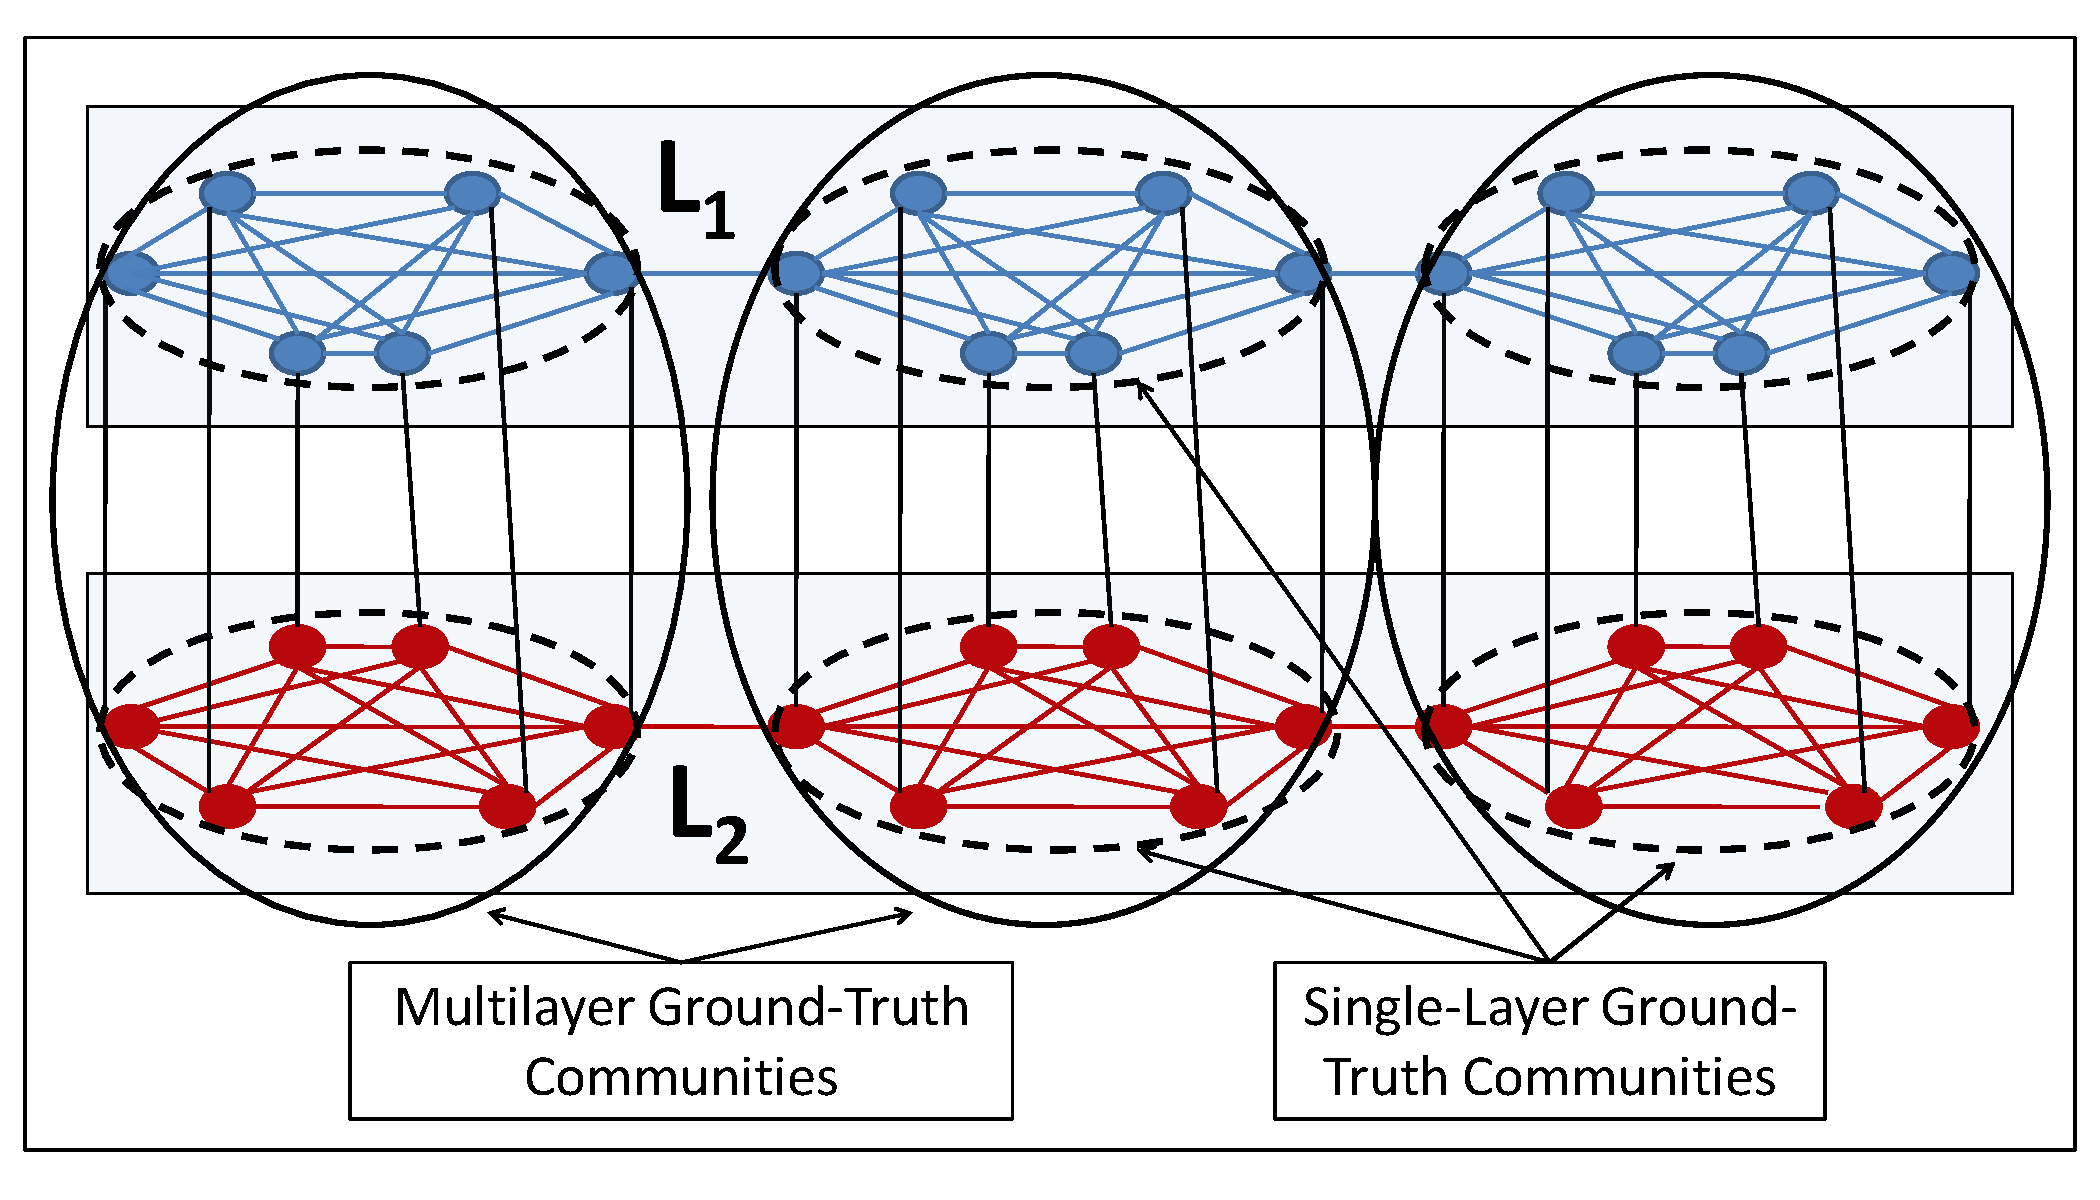
\includegraphics[width=2.5in]{./images/image31.pdf}
% \vspace{-0.1in}
% \caption{Network configuration with two different ground truth communities}
% \label{N0}
% \end{figure}

\subsection{Experimental Results}
In our experiment, we increase the coupling edge density $d$ from $0$ to $1$, for both the ground truth configurations A \& B,
with different $p$ values.
Intuitively, addition of coupling edges should dilute the single layer community structures in Config A, decreasing the
modularity of Config A, whereas in Config B, it should make the cross layer
communities more cohesive, increasing the modularity.

\subsubsection{Config A}
In Fig.~\ref{cross_single} the plot corresponding to $mQ$ reveals that it is completely insensitive 
to the increase in
coupling edge density $d$. Precisely, in case of Config A the coupling edges
do not have any contribution in Eq.~\ref{eq_mQ} (coupling edge term vanishes for single layer communities),
hence $mQ$ remains invariant against addition of
coupling edges. On the contrary, in case of $Q_M$, we penalize for the coupling edges connected with single layer
communities (see $(h_i+\theta_{C_k}*c_i)$ terms in Eq.~\ref{final1}) which allows us to achieve the drop in $Q_M$ values with 
increasing $d$ (see
Fig.~\ref{cross_single}). This result concurs with the desired $Property^S$, introduced in section~\ref{prop}. 
%Config A does not have any cross layer community; so both the plots in Fig.~\ref{cross_single} are invariant with $p$.

% \begin{figure}
% \centering
% 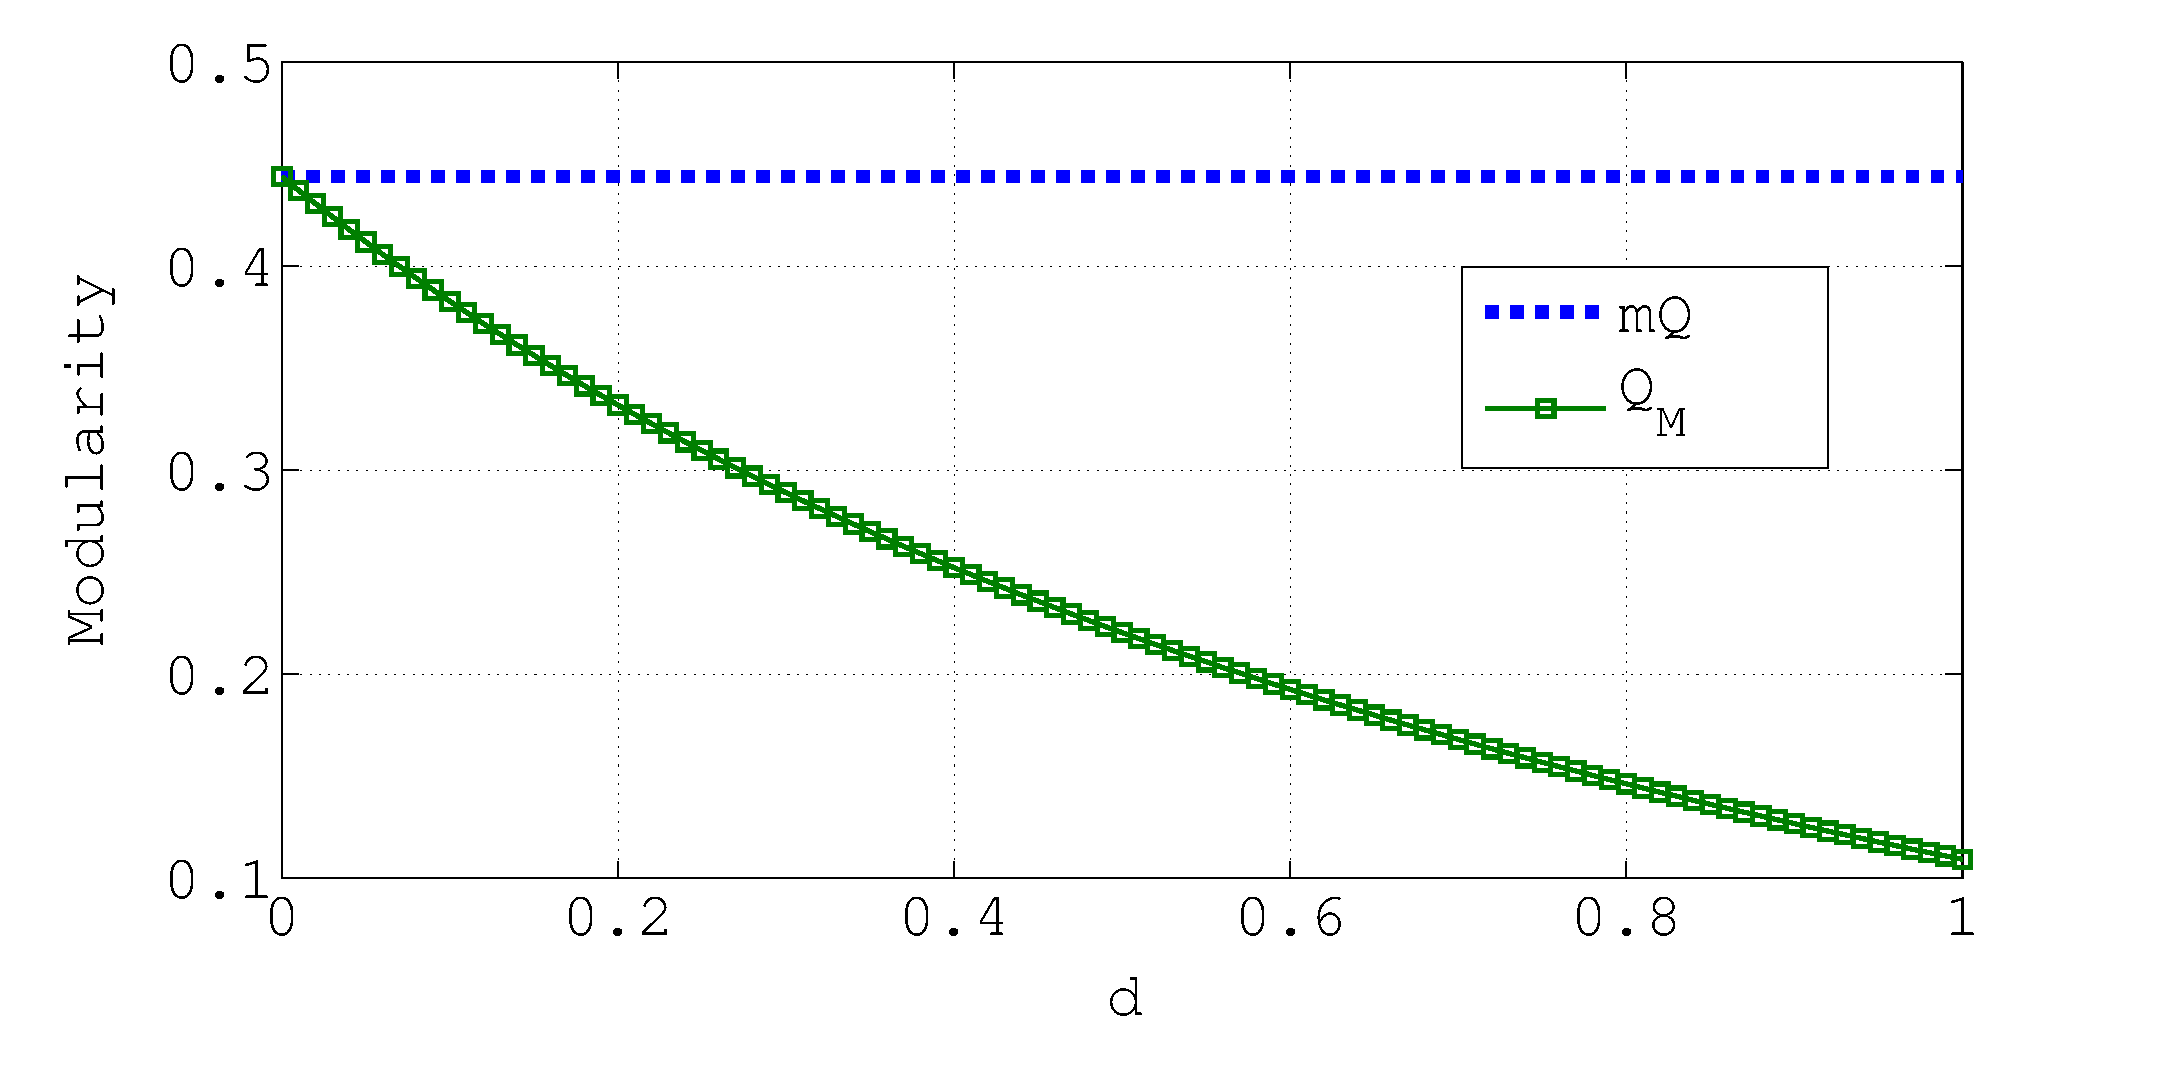
\includegraphics[width=2.5in]{./images/mQ_vs_march21_cross_single.pdf}
% \vspace{-0.1in}
% \caption{Comparison of $mQ$ and $Q_M$ for Config A while adding coupling edges with different $P$ values}
% \label{cross_single}
% \end{figure}

\subsubsection{Config B}
In case of Config B, $mQ$ is unable to capture the desired increasing behavior (see $Property^X$, introduced in section~\ref{prop}) with
the increase in coupling edges (except at
the beginning when $d$ becomes non-zero for the first time). Rather, it remains constant throughout the edge addition
regime irrespective of the $p$ values (see Fig.~\ref{cross_multi}).
In Config B, as observed from Eq.~\ref{eq_mQ}, the coupling edge addition only affects the 
term for coupling edges
%bipartite modularity term [BM: what is this term in eq 7? term for coupling edges? Then write it directly] 
of $mQ$;
however, addition of edges influences the numerator and denominator almost equally, neutralizing the overall effect on $mQ$.
%Essentially, here the major deficiency of modularity $mQ$ stems from the fact that it evaluates the quality of a cross layer community
%by individually checking its single layer and bipartite components without verifying how well the individual single layer components within each cross layer community are connected with each other.
On the other hand, in all the plots corresponding to $Q_M$, the modularity increases gracefully with coupling
edge addition. This is achieved by suitably penalizing the null model in Eq.~\ref{eq_multi}.
%This is due to the consideration of intra layer degrees of nodes which are not connected via coupling edges in the middle term of $Q_M$ (see Eq.~\ref{final1}) which helps to penalize the bipartite modularity for having such nodes in the community.
As expected, the absolute value of modularity increases with $p$ for both $mQ$ and $Q_M$, since higher $p$ improves the cohesiveness
of cross layer communities.

% \begin{figure}
% \centering
% 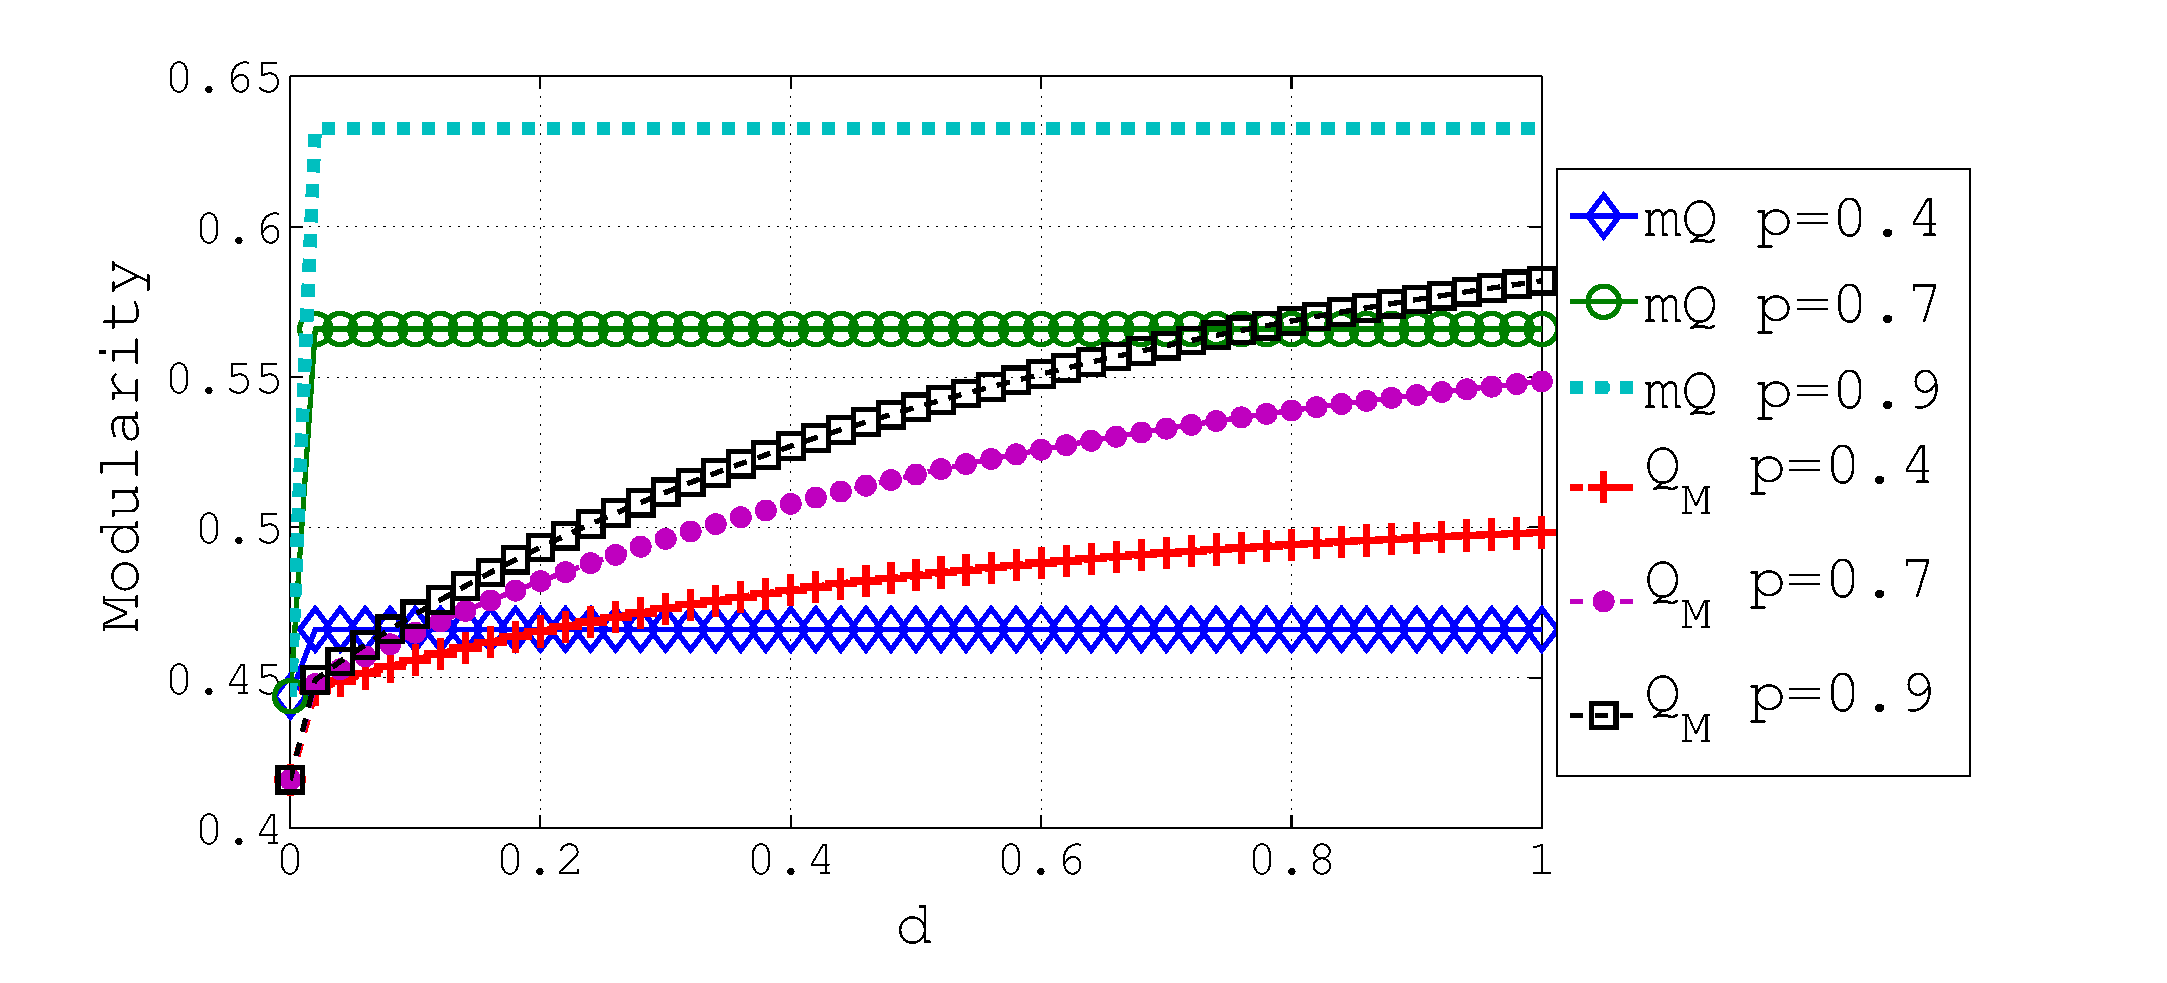
\includegraphics[width=3.5in]{./images/mQ_vs_march21_cross_multi.pdf}
% \vspace{-0.1in}
% \caption{Comparison of $mQ$ and $Q_M$ for Config B while adding coupling edges with different $P$ values}
% \label{cross_multi}
% \end{figure}

In a nutshell, the aforesaid experiments clearly demonstrate the elegance of $Q_M$ with respect to $mQ$, as a community quality index.
%In the next two sections, we evaluate how efficiently we can discover communities with the help of $Q_M$ in synthetic and empirical multilater networks.

% % We illustrate this limitation with the help of a representative example.
% % (a) We introduce the factors $e^{-F^C_1}$ and $e^{-F^C_2}$, respectively with the corresponding single layer modularity terms.
% % Consider a community $L^C_1$ which is very cohesive in the $L_1$ layer itself, however a high fraction of
% % nodes in $L^C_1$ may also be connected with the nodes of some different community of layer $L_2$ through coupling
% % edges (high $F^C_1$); this should dilute the cohesiveness of community $L^C_1$ and penalize the overall modularity.
% % Hence, we introduce the factors $e^{-F^C_1}$ and $e^{-F^C_2}$ to penalize the single layer terms of modularity.
% % Fig.~\ref{single1} depicts that in Config A, modularity
% % $MultiMod$ gracefully improves as a result of removal of these type of coupling edges.
% %
% % (b) The factor $H^C_1\times H^C_2$, introduced with the coupling layer term of Eq.~\ref{eqn2}, measures how strongly the coupling
% % edges in community $C$ connect the group of nodes
% % $L^C_1$ and $L^C_2$ respectively. In Config B, even if the cross layer term results in high modularity, removal
% % of coupling edges results in low $H^C_1\times H^C_2$, which in turn reduces $MultiMod$. In Fig.~\ref{single0}, we can
% % observe that in Config B, $MultiMod$ gracefully degrades, following our intuition, with deletion
% % of coupling edges.



%\subsection{Ranking Algorithms}



%\subsection{Sensitivity} 
\section{Community Evaluation: Synthetic network}
\label{eval}
We evaluate the performance of the proposed multilayer community detection algorithms \textbf{GN-$Q_M$} and \textbf{Louvain-$Q_M$} in a
controlled environment. First we present the experimental setup explaining the generation of synthetic multilayer network
with ground truth communities and the evaluation metric. Next, we present the competing baseline algorithms and
finally, we exhibit the elegance of the proposed algorithms over baselines from different perspectives.
% Additionally, we also discuss about the scalability \& adaptability of our algorithm for larger and more
% complicated network [BM: do we really want it?] structures.

\subsection{Experimental setup}
We generate the synthetic two layer networks ($\mathcal{G} = \{\{L_1, L_2\}, \{L_{12}\}\}$) with planted communities
following the model proposed in section~\ref{syn_gen}.
We fix the number of nodes $|V_i|$ in each layer $L_i$ at $100$ with maximum degree $k^{i}_{max}=10$ \& average
degree $\langle k_i\rangle=6$. The power-law exponents for degree distribution ($\gamma_i$) and community size distribution ($\beta_i$)
for each layer are fixed at 2 and 1 respectively.
The other model parameters ($\mu$, $\alpha$, $p$ \& $d$) are regulated and adjusted according to the requirement.
We apply the normalized mutual information (NMI)~\cite{danon2005comparing} as the yardstick
to quantify the similarity between the detected and ground truth communities.
% Suppose, $N$ is the number of nodes in the entire multilayer network,
% $w_1, w_2, \dots, w_W$ are the sets of nodes (all layers combined) contained in the
% detected $W$ communities and $r_1, r_2, \dots, r_R$ are the sets of nodes (all layers combined) contained in the
% total $R$ ground truth communities.
% Then NMI, of this two sets of communities can be calculated as
%
% \begin{equation}
%  NMI = \frac{\sum_{k=1}^{W} \sum_{j=1}^R \frac{\left \vert w_k \cap r_j \right \vert}{N} \log \frac{N \left \vert w_k \cap r_j \right \vert}
%  {\left \vert w_k \right \vert \left \vert r_j \right \vert}} {[(-\sum_{k=1}^W\frac{\left \vert w_k \right \vert}{N}
%  \log \frac{ \left \vert w_k \right \vert}{N} ) + (-\sum_{j=1}^R \frac{\left \vert r_j \right \vert}{N}
%  \log \frac{ \left \vert r_j \right \vert}{N})]/2}
% \end{equation}
%
%$NMI$ attains higher value if the ground truth and detected communities exhibit good agreement.
The synthetic network contains $30$
single layer (\& no cross layer) ground truth communities when $\alpha = 0$ and $15$
cross layer (\& no single layer) ground truth communities when $\alpha = 1$.

%If both match completely, we have a maximum NMI value of 1, whereas if the obtained and ground truth partitions are totally independent of one another, we have a minimum value of 0. Such kind of testing is widely used by other researchers in the community detection field[CITE?].


% \begin{figure}
% \centering
% 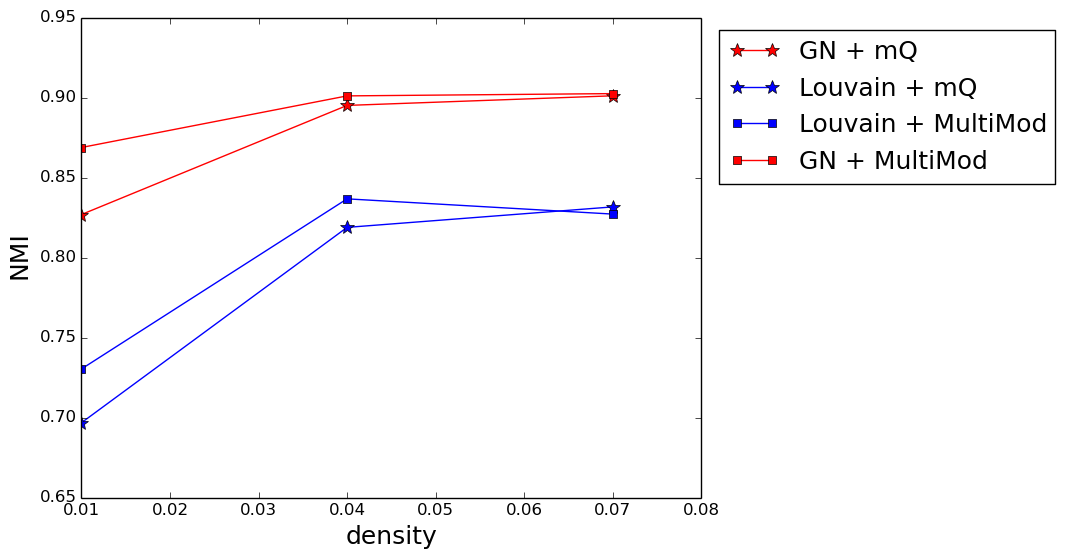
\includegraphics[width=3.5in]{./images/NMI_D_P0_4_A0_6_MU0_05.png}
% \vspace{-0.1in}
% \caption{NMI of obtained and ground truth communities various $d$ values for $p=0.4$, $\alpha=0.6$, $\mu=0.05$}
% \vspace{-0.1in}
% \label{nmi1}
% \end{figure}
\subsection{Competing algorithms}
%As we mentioned before, any single layer community detection algorithm which maximizes modularity or a similar metric can be used as
%our algorithm. In this paper, we choose Girvan-Newman~\cite{newman2004fast} (GN) and Louvain~\cite{blondel2008fast} as our
%single layer algorithms on top of which we use our $Q_M$ metric. We compare this two methods with the following two types of
%baseline methods.
% [BM: Use the following naming convention; \textbf{GN-$Q_M$}, \textbf{Louvain-$Q_M$}, \textbf{GN-$mQ$} and
% \textbf{Louvain-$mQ$} etc]
We introduce the following three classes of competing algorithms to evaluate the
performance of \textbf{GN-$Q_M$} and \textbf{Louvain-$Q_M$}.

\subsubsection{Baselines with $mQ$} We induce the multilayer modularity $mQ$ proposed in~\cite{medical_paper} with the standard
 Girvan-Newman and Louvain algorithms~\cite{newman2004finding},~\cite{blondel2008fast}. We refer these baseline algorithms 
 as \textbf{GN-$mQ$} and \textbf{Louvain-$mQ$} respectively.

\subsubsection{Merging based baselines} We apply standard Louvain algorithm~\cite{blondel2008fast} to
 detect communities at the individual layers and then attempt to merge those communities across the layers.
 We merge one top layer community $C_T$ with one bottom layer community $C_B$ with which it is maximally connected 
 if the connection density between them is above a threshold\footnote{Merging is performed if the ratio of the number of coupling links 
 between $C_T$ \& $C_B$ and the total number of 
 coupling links connected with $C_T$ \& $C_B$ is at least $Th$. We vary $Th$ from $0.1$ to $1.0$ and report the best obtained result.}; 
 otherwise keep $C_T$ and $C_B$ as a single layer community.

\subsubsection{State-of-the-art algorithms} We implement `MetaFac'~\cite{metafac} and `CompMod'~\cite{CompMod} as state of the art multilayer community
detection algorithms, already introduced in section~\ref{syn_evalu}.

\begin{figure}
\begin{center}
\subfigure[Varying $d$ values for $p=0.4$, $\alpha=0.6$, $\mu=0.05$ for $mQ$ based baselines
]{\label{nmi1}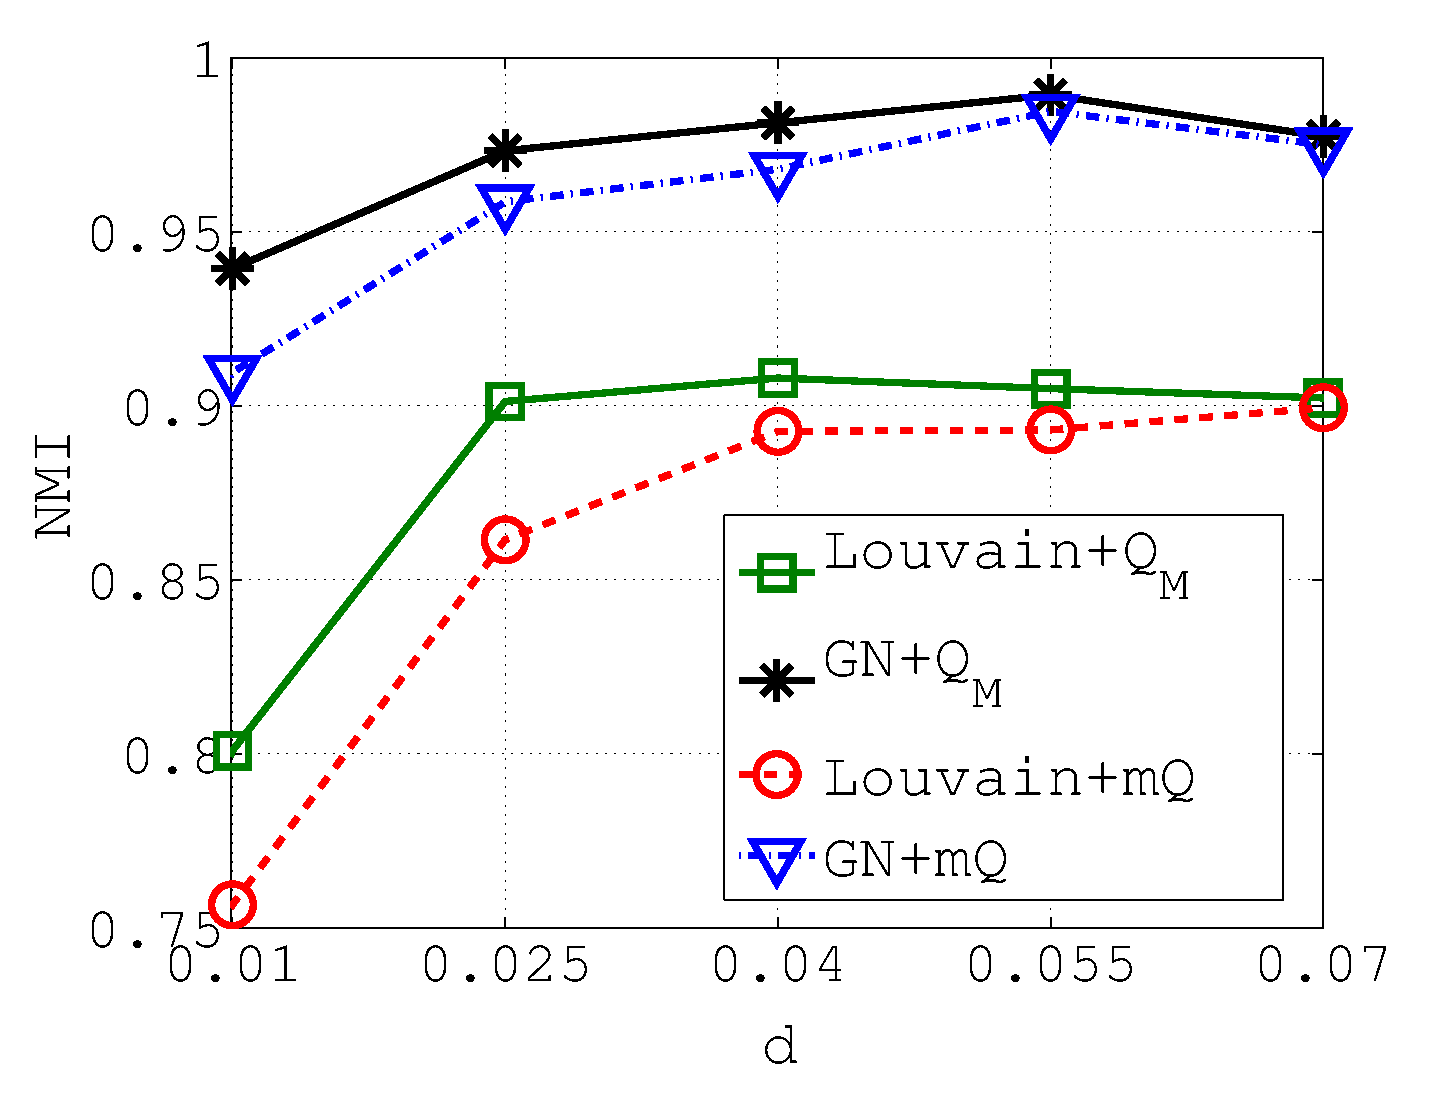
\includegraphics[angle=0,scale=.17]{./images/NMI_density_mQ_QM.pdf}}
\subfigure[Varying $d$ values for $p=0.4$, $\alpha=0.6$, $\mu=0.05$ for merging based baselines
]{\label{nmi1_1}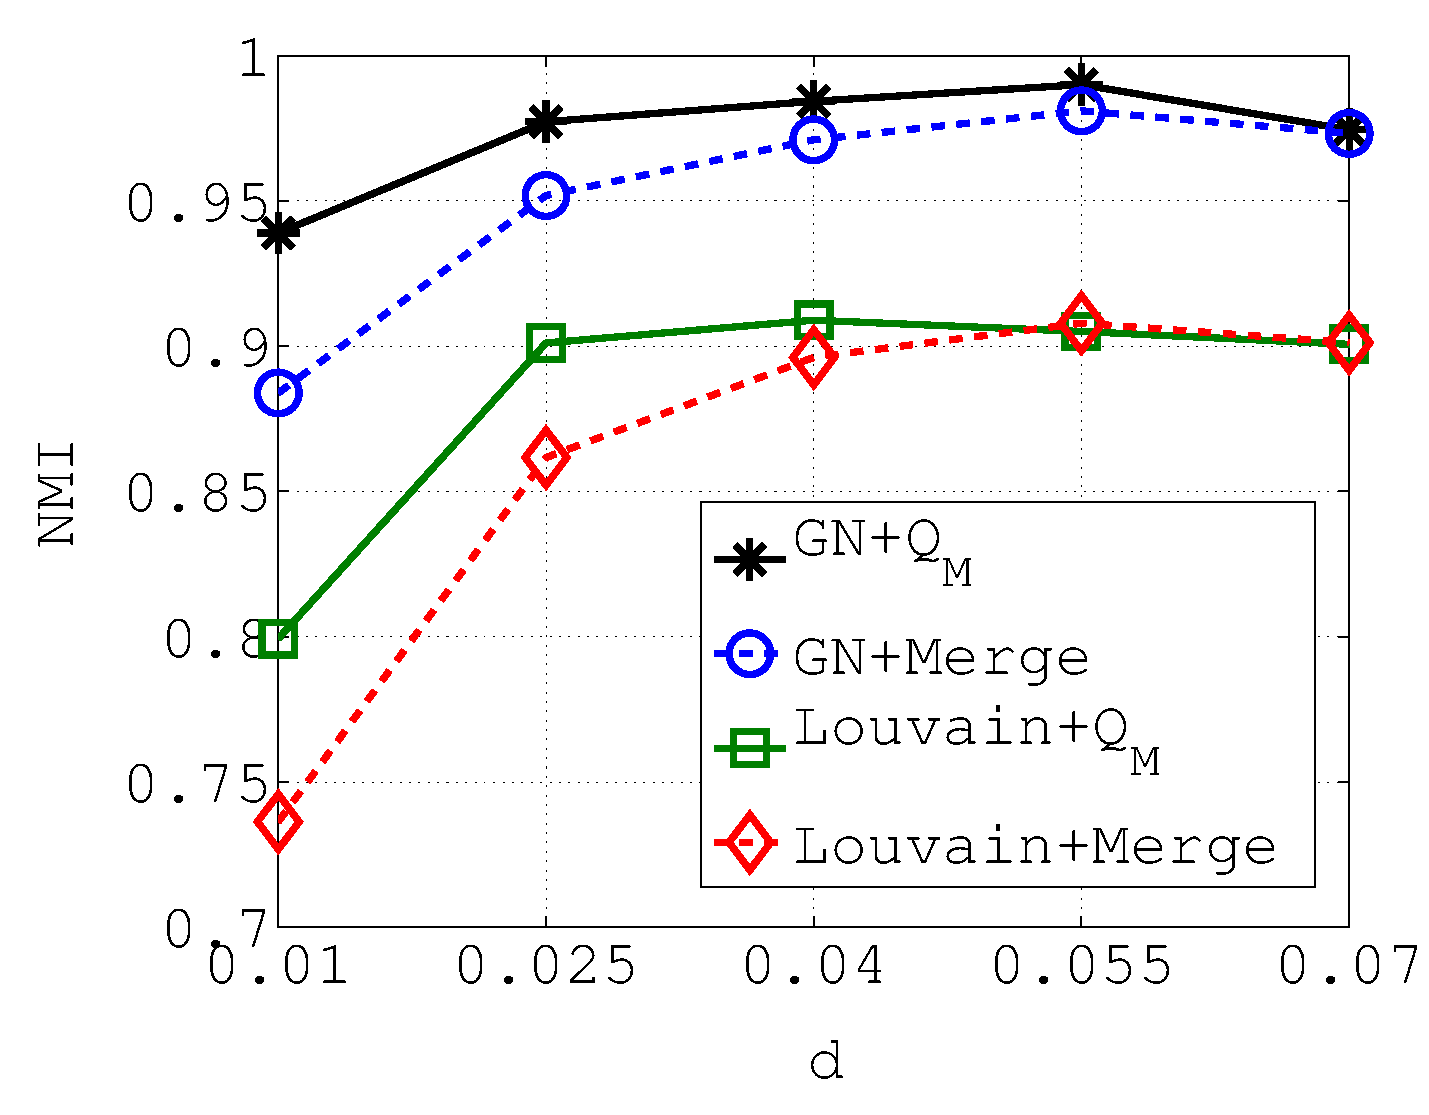
\includegraphics[angle=0,scale=.17]{./images/NMI_density_merge_QM.pdf}}
\end{center}
\vspace{-0.24in}
\caption{NMI of obtained and ground truth communities for various $d$ values.}
\vspace{-0.22in}
\label{nmi00}
\end{figure}



% \begin{figure}
% \begin{center}
% \subfigure[Precision
% ]{\label{reco1}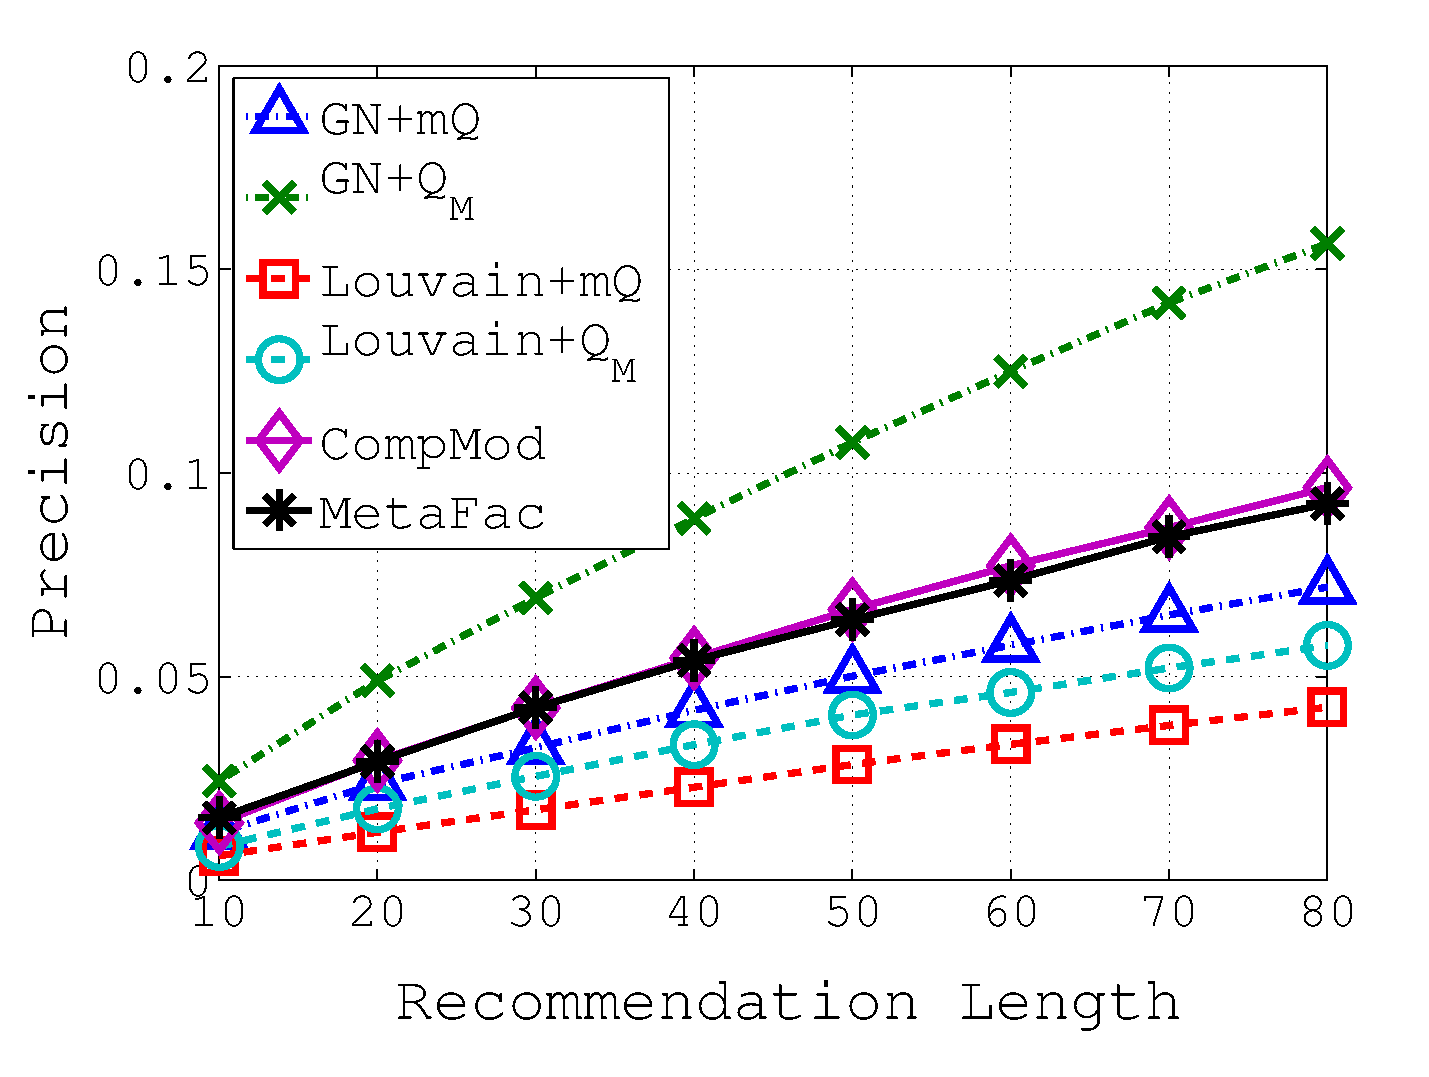
\includegraphics[angle=0,scale=.18]{./images/Intersection_Reco_march21_square.pdf}}
% \subfigure[F1 Score
% ]{\label{reco0}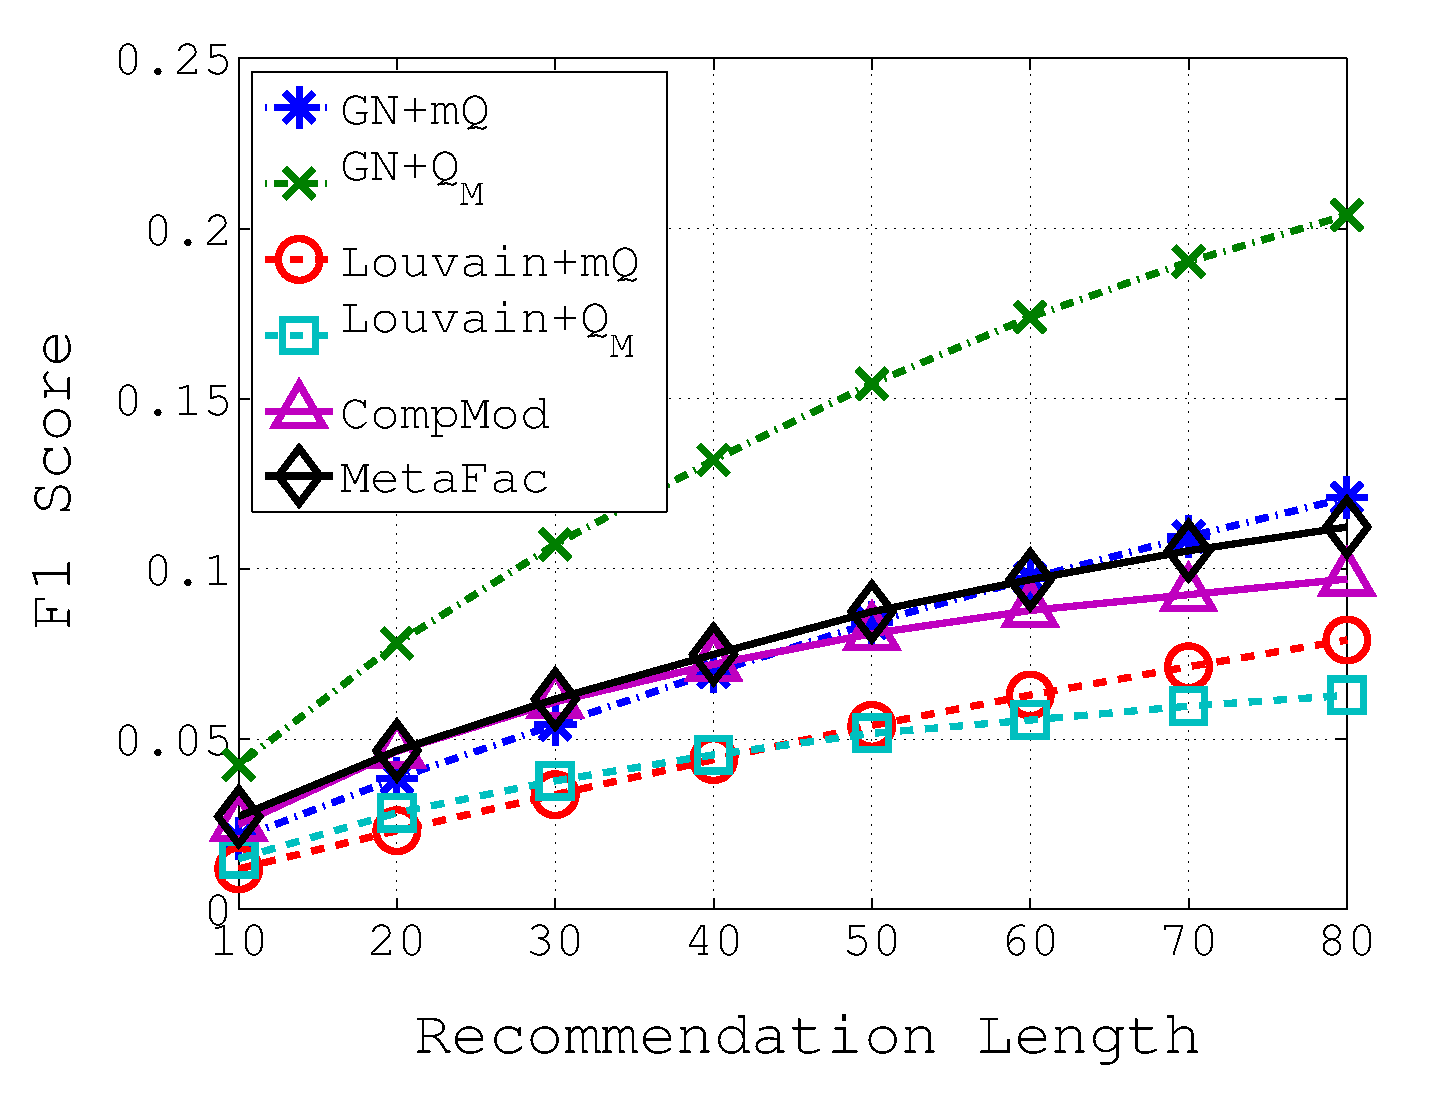
\includegraphics[angle=0,scale=.18]{./images/F1_Reco_march21_square.pdf}}
% \end{center}
% \vspace{-0.3in}
% \caption{Precision \& F1 Score for communities obtained from different algorithms for various recommendation lengths}
% \vspace{-0.22in}
% \label{reco}
% \end{figure}

\subsection{Evaluation}
\subsubsection{Comparison with baselines with $mQ$}
The proposed \textbf{GN-$Q_M$} and \textbf{Louvain-$Q_M$} algorithms perform quite closely with their respective benchmark 
\textbf{GN-$mQ$} and
\textbf{Louvain-$mQ$}  However, the improvement gets manifested when we reduce the density
of coupling links $d$. In Fig.~\ref{nmi1}, we observe that \textbf{GN-$Q_M$} and \textbf{Louvain-$Q_M$} outperform the baselines in the
lower link density regime. This comes from the fact that the modularity $mQ$ fails to reflect the cohesiveness
of multilayer communities for low $d$ values, as explained in Fig.~\ref{cross_multi}.

\subsubsection{Comparison with merging based baselines}
This baseline
%\footnote{For each configuration, we vary the threshold of merging and depict the one giving the best NMI.} 
performs pretty close to aforesaid \textbf{GN-$mQ$} and \textbf{Louvain-$mQ$}  since here
also we optimize the
modularities at top, bottom and bipartite layers separately. Evidently, the proposed \textbf{GN-$Q_M$} and \textbf{Louvain-$Q_M$} 
algorithms outperform
this baseline in the low coupling link density ($d$) regimes (see Fig.~\ref{nmi1_1}).

%Hence, as expected, the merging based baselines perform quite closely with the corresponding
% and fails to reflect the cohesiveness of multilayer communities in $d$, as explained in Fig.~\ref{single0}. The higher NMI of \textbf{GN-$Q_M$} and Louvain-$Q_M$
% manifests the elegance of the proposed modularity index $Q_M$.


\subsubsection{Comparison with state-of-the-art algorithms}
% \begin{figure}
% \centering
% 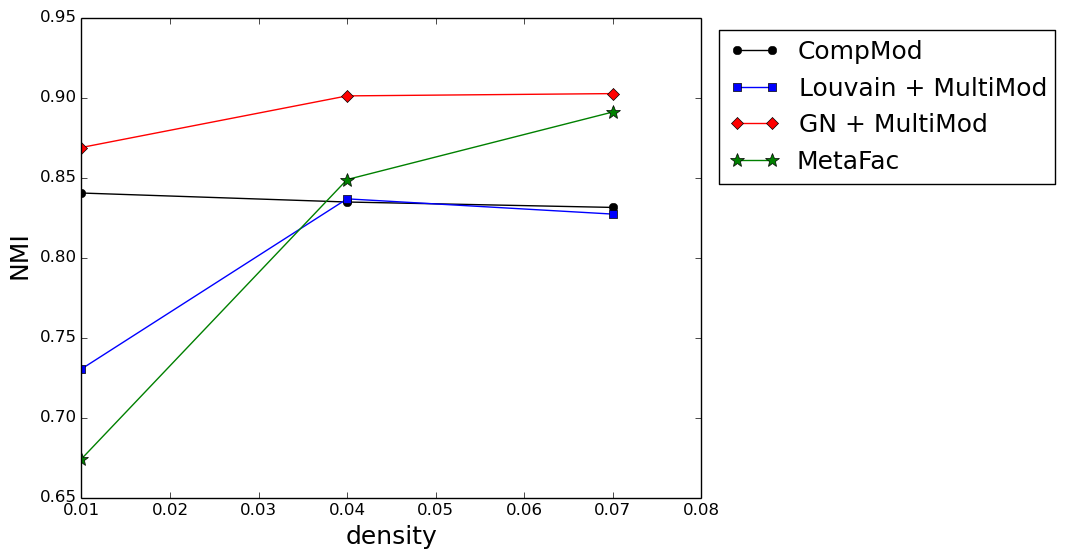
\includegraphics[width=3.5in]{./images/NMI_D2_P0_4_A0_6_MU0_05.png}
% \vspace{-0.1in}
% \caption{NMI of obtained (nmi for mQ and nmia for $Q_{adapt}$) and ground truth communities for p=0.9}
% \vspace{-0.1in}
% \label{nmi}
% \end{figure}

\textbf{(a) Effect of $\alpha$:} The model parameter $\alpha$ regulates the proportion of ground truth cross layer
(against single layer) communities in the
 synthetic multilayer network. In Fig.~\ref{nmi2}, we observe that \textbf{GN-$Q_M$} and \textbf{Louvain-$Q_M$} do not exhibit high
 sensitivity with $\alpha$; this points to the
 fact that performance of these two algorithms (specially GN-$Q_M$) does not depend on the proportion of single layer
 and cross layer communities present in the network. However, the performance of $MetaFac$ monotonically improves
 with increasing $\alpha$ whereas $CompMod$
exhibits the opposite behaviour. In fact, $MetaFac$ algorithm is intrinsically biased towards detecting cross layer
communities whereas
 $CompMod$ is more suitable for detecting single layer communities.
\textbf{(b) Effect of $p$:}  Model parameter $p$ realizes the cohesiveness of the coupling links in the apriori cross layer communities.
We observe (see Fig.~\ref{nmi4}) that our algorithms outperform $MetaFac$ and $CompMod$ in the presence of moderate to cohesive 
cross layer communities (say $p>0.3$). However, for $p<0.3$ $CompMod$ performs relatively better due to the degradation of
the cross layer communities, since $CompMod$ intrinsically favors the single layer communities.

\begin{figure}
\begin{center}
\subfigure[Varying $\alpha$ values for $p=0.8$, $\mu=0.4$ and $d=0.04$
]{\label{nmi2}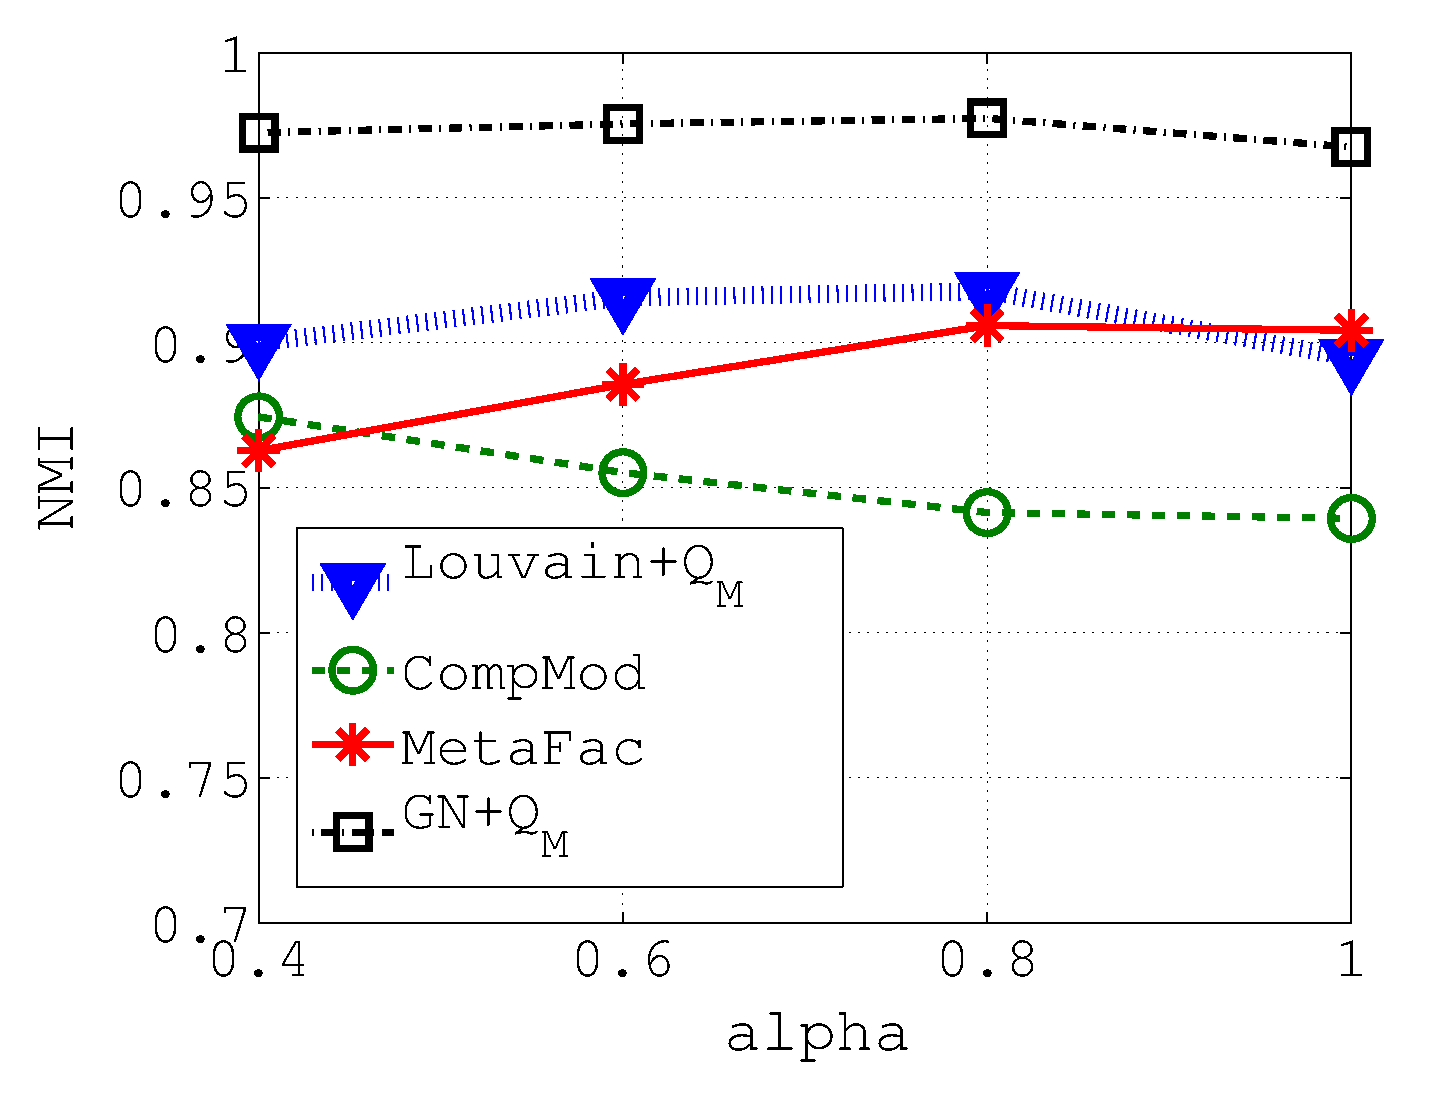
\includegraphics[angle=0,scale=.17]{./images/NMI_alpha_QM.pdf}}
% \subfigure[Varying $\mu$ values for $p=0.8$, $\alpha=0.6$ and $d=0.04$
% ]{\label{nmi3}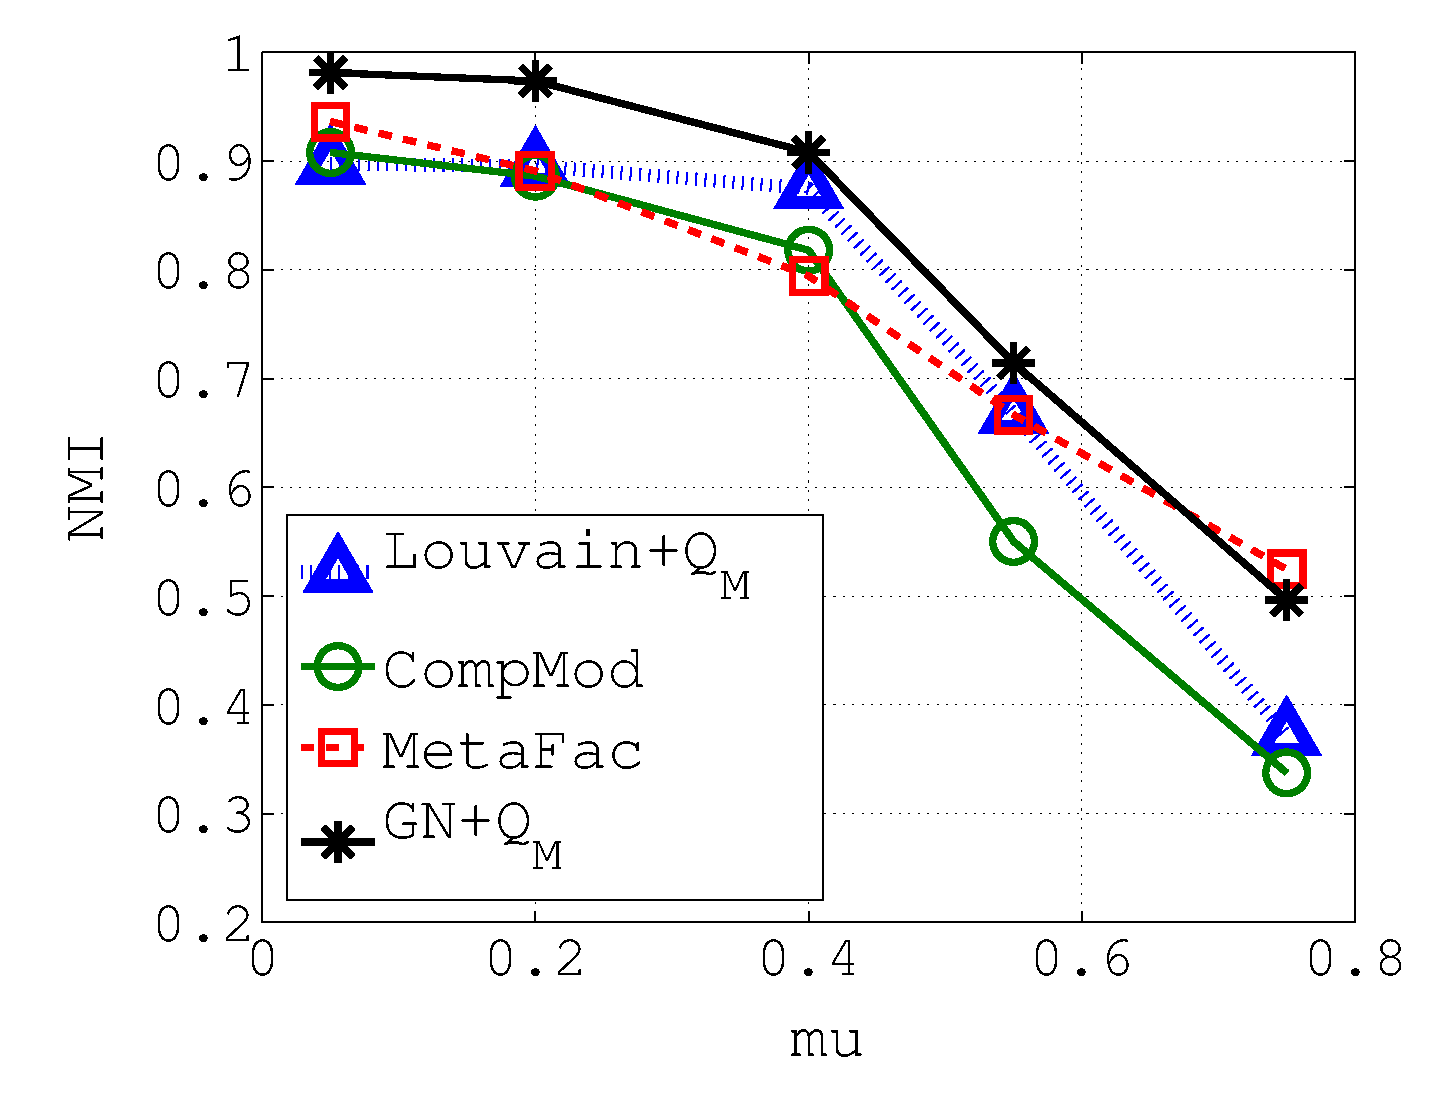
\includegraphics[angle=0,scale=.21]{./images/NMI_mu_QM.pdf}}
\subfigure[Varying $p$ values for $\mu=0.4$, $\alpha=0.6$ and $d=0.04$
]{\label{nmi4}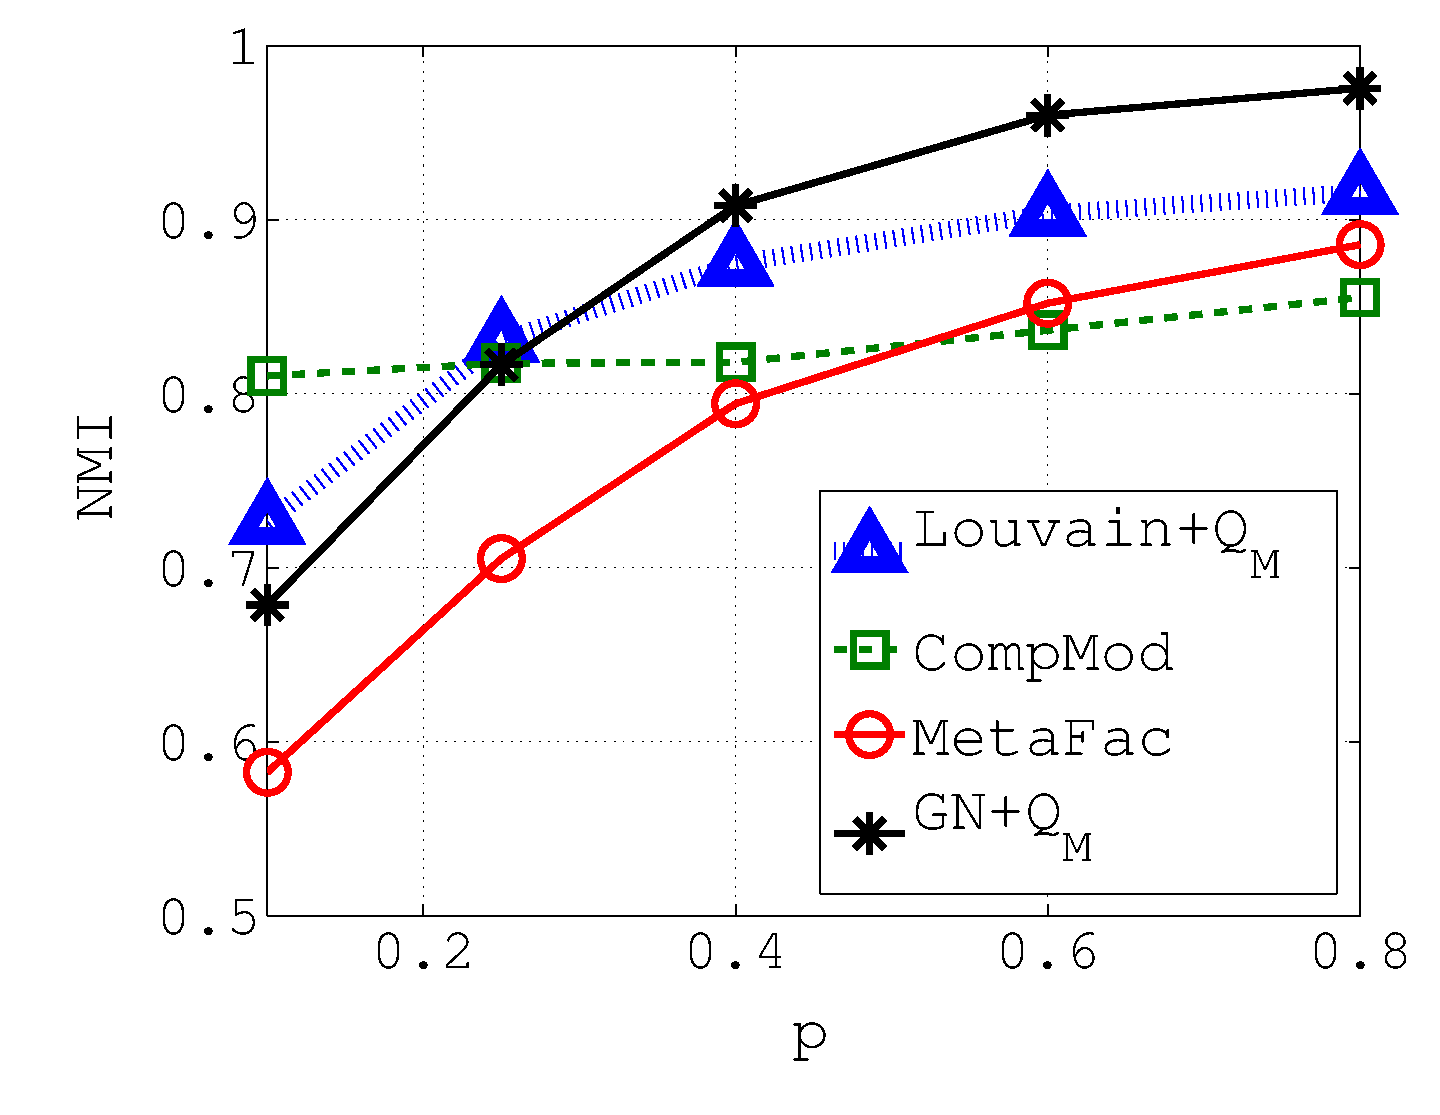
\includegraphics[angle=0,scale=.17]{./images/NMI_p_QM.pdf}}.
\end{center}
\vspace{-0.23in}
\caption{NMI of obtained and ground truth communities for various $\alpha$ \& $p$ values.}
\vspace{-0.25in}
\label{nmi11}
\end{figure}


% \begin{figure}
% \centering
% 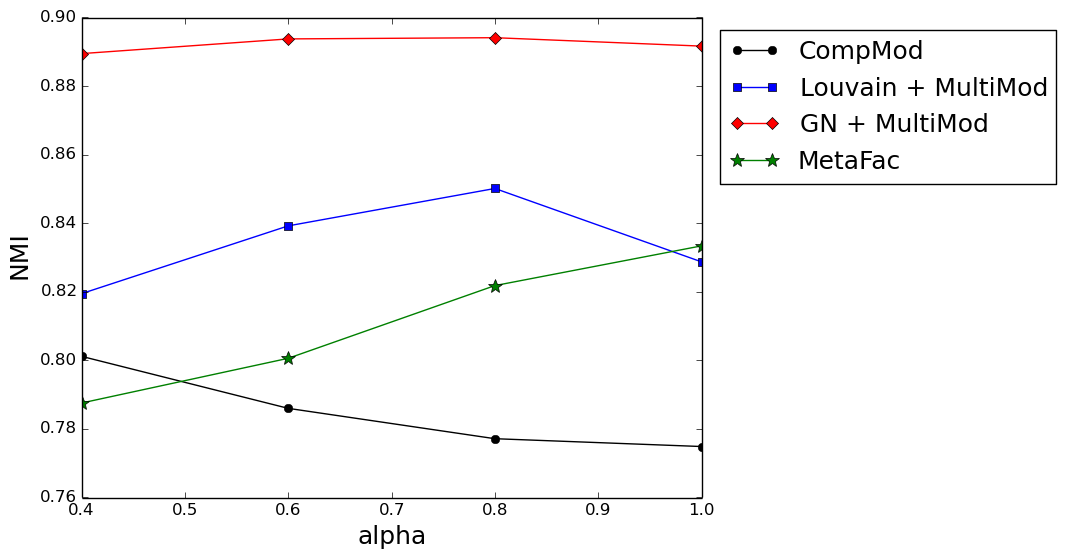
\includegraphics[width=3.5in]{./images/NMI_A_P0_8_MU0_4_D0_04.png}
% \vspace{-0.1in}
% \caption{NMI of obtained and ground truth communities with various $\alpha$ values for $p=0.8$, $\mu=0.4$ and $d=0.04$}
% \vspace{-0.1in}
% \label{nmi2}
% \end{figure}

% \item Effect of $\mu$: $\mu$ is the LFR parameter which decides the cohesivity of the single layer communities in the
% first step of synthetic network generation; increasing $\mu$ degrades the community cohesivity.
% We observe decreasing NMI for all the algorithms with increasing $\mu$ in Fig.~\ref{nmi3}.
% Nevertheless, \textbf{GN-$Q_M$} performs marginally better than competing algorithms.
% This is possibly because higher $\mu$ indicates poor cohesiveness; hence, poor quality of ground
% truth communities.



% \begin{figure}
% \centering
% 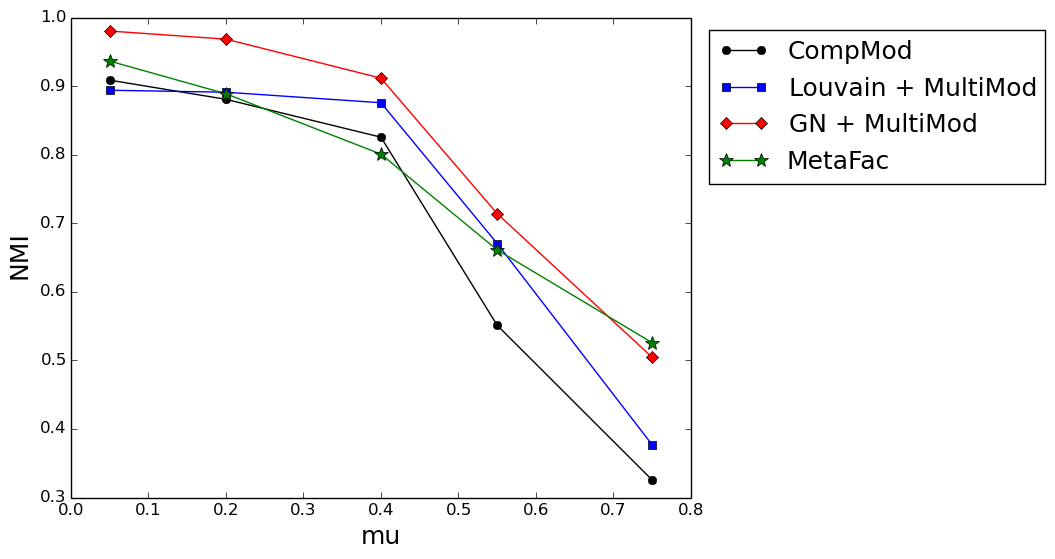
\includegraphics[width=3.5in]{./images/NMI_MU_P0_4_A0_6_D0_04.png}
% \vspace{-0.1in}
% \caption{NMI of obtained and ground truth communities with various $\mu$ values for $p=0.8$, $\alpha=0.6$ and $d=0.04$}
% \vspace{-0.1in}
% \label{nmi3}
% \end{figure}

% \begin{figure}
% \centering
% 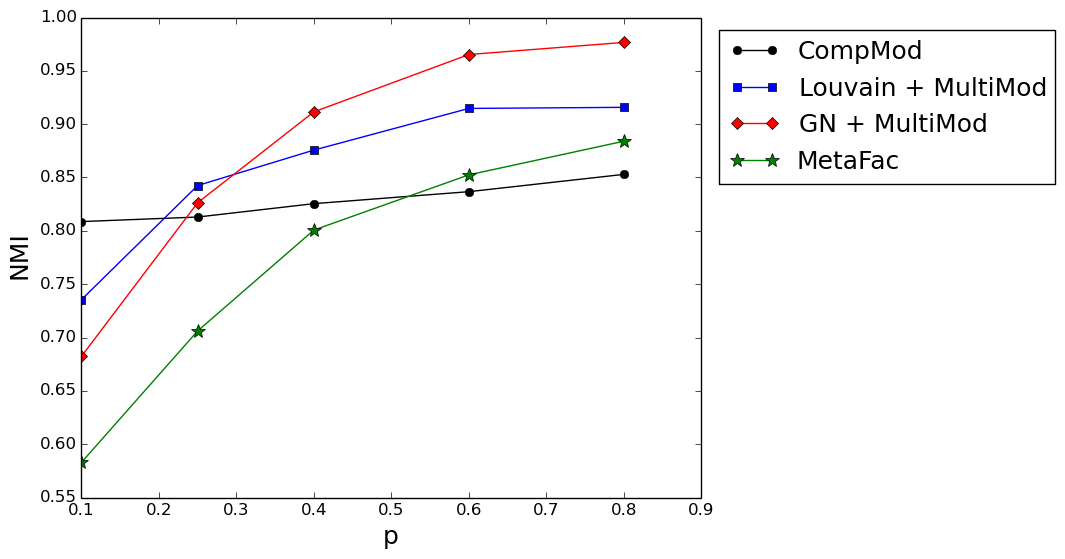
\includegraphics[width=3.5in]{./images/NMI_P_A0_6_MU0_4_D0_04.png}
% \vspace{-0.1in}
% \caption{NMI of obtained and ground truth communities with various $p$ values for $\mu=0.4$, $\alpha=0.6$ and $d=0.04$}
% \vspace{-0.1in}
% \label{nmi4}
% \end{figure}


%[BM: check. dropped $\mu$]
In a nutshell, we claim that (a) the proposed algorithms show pretty balanced behaviour across different range of model
parameters ($d$, $p$ etc) and (b) importantly, they can
simultaneously detect both single layer and cross layer communities without any specific bias towards anyone of 
them (invariant to $\alpha$).
Though \textbf{GN-$Q_M$} and \textbf{Louvain-$Q_M$} perform relatively poorly in the lower $p$ regions, notably, they never rank as the
worst in the batch. $CompMod$ performs decently in lower $p$ regions due to its intrinsic bias towards cross layer communities,
where $MetaFac$ fails miserably.

%R[BM: In the entire paper, replace cross layer link as coupling link.]

% \subsection{Comparison with baselines}
% Compare the results produced by different baselines on different synthetic networks with our algorithm's results. We
% may use different metrics like NMI, ARI, Purity etc. and their weighted versions \cite{metric} for comparisons. We
% need to also explain the reason of the success of our algorithm and modularity metric. The baseline algorithms can be the ones used in
% \cite{InfoCom} (CompMod~\cite{CompMod}, MetaFac~\cite{metafac}, NaiveSimp, Trans-C, Trans-JD),
% the algorithm InfoCom proposed in ~\cite{InfoCom} itself
% and the algorithm proposed in ~\cite{medical_paper}.\textcolor{red}{[SP: I have already received the code for CompMod~\cite{CompMod}. If
% Raphael can implement InfoCom~\cite{InfoCom} and MetaFac~\cite{metafac} (at least the MetaFac), it will be very helpful. Implementing others
% are relatively trivial.]}
%
% \subsection{Effect of varying Parameters}
% In this subsection, we apply the Newman-Girvan community detection algorithm with modularity replaced by $mQ$ and $Q_{adapt}$ on different
% synthetic networks generated with different parameters. This is done to analyze the impact of those parameters on the ground
% truth and obtained communities. In general, the communities obtained by maximizing $mQ$ and $Q_{adapt}$ are very similar
% irrespective of the synthetic network parameters.
%
% \begin{figure}
% \begin{center}
% \subfigure[Modularity of Ground Truth communities (Qt) and communities obtained using $mQ$ as a metric (Q) and
% using $Q_{adapt}$ as a metric (Qa) at p=0.9
% ]{\label{Q1}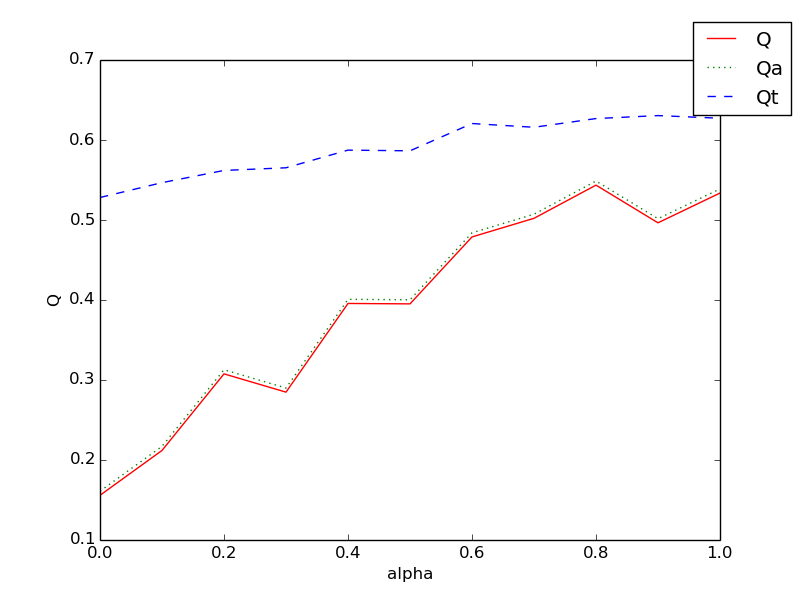
\includegraphics[angle=0,scale=.25]{./images/Q0_9.png}}
% \subfigure[Modularity of obtained communities using $mQ$ as a metric (Q) and
% using $Q_{adapt}$ as a metric (Qa) removing a fraction $g$ of cross community coupling edges at p=0.7.
% ]{\label{Q2}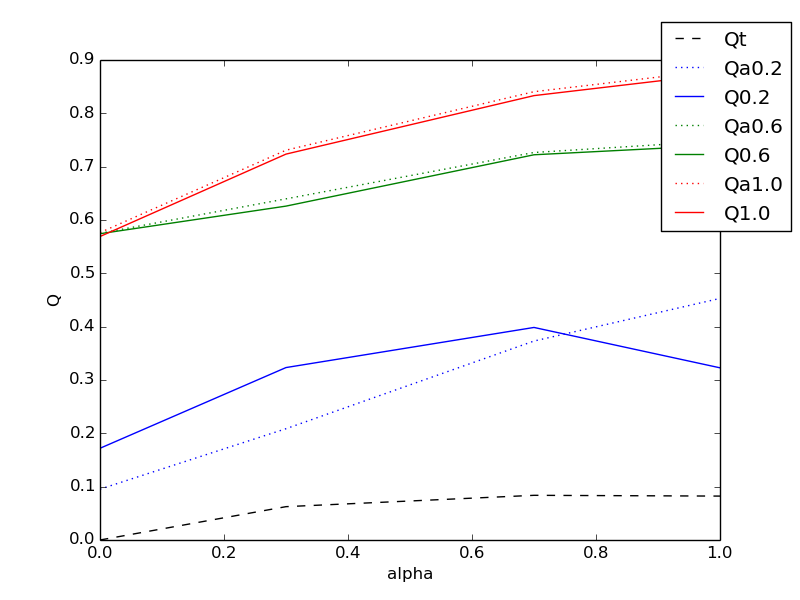
\includegraphics[angle=0,scale=.25]{./images/Q0_7_mp0_65.png}}
% \end{center}
% \vspace{-0.22in}
% \caption{Modularity of Ground Truth and obtained communities}
% \label{Q}
% \end{figure}
%
%
%
%
% \begin{enumerate}
%  \item \textbf{Effect of $p$ and $\alpha$ on modularity:} We observe that if $p$ is high i.e. most of the coupling edges are within
%  cross-layer communities, then modularity of the ground truth communities as well as obtained communities increase
%  with $\alpha$ (fraction of multilayer communities in ground truth)
%  (see Fig.~\ref{Q1}). This happens because high $\alpha$ implies that most of the ground-truth communities are multilayer and
%  high $p$ implies that most of the multilayer communities are of good quality. This two factors jointly help to increase the modularity
%  of the ground truth and obtained communities. The opposite occurs when $p$ is low i.e. modularity decreases with increasing $\alpha$ in
%  that case.\\
%  \item \textbf{Effect of deleting fraction of cross community coupling edges on modularity:} A disadvantage of our synthetic network
%  generation procedure is that we cannot fully control the number of coupling edges. The parameter $p$ just controls the fraction
%  of coupling edges within and outside the cross-layer communities. In general, the count of
%  cross community coupling edges is quite high with respect to the amount of single layer edges. This disrupts the cross-layer
%  community structure and lowers the modularity for ground truth and obtained communities.
%  If we remove a fraction $g$ of cross community coupling edges before running the community
%  detection algorithm, the modularity of the obtained communities improve (see Fig.~\ref{Q2}). The reason is intuitive - removing
%  cross community coupling edges essentially improves the quality of the cross-layer communities. The obtained communities even have higher
%  modularity than the ground truth communities.\\
%
% \begin{figure}
% \begin{center}
% \subfigure[CDF of different types of deleted edges while running Newman-Girvan algorithm with iterations for
% mixing parameter 0.05, p=0.7 and $\alpha$=0.7
% ]{\label{d1}\includegraphics[angle=0,scale=.25]{./images/mp05_0_7_0_7_0_2.png}}
% \subfigure[CDF of different types of deleted edges while running Newman-Girvan algorithm with iterations for
% mixing parameter 0.65, p=0.7 and $\alpha$=0.7
% ]{\label{d2}\includegraphics[angle=0,scale=.25]{./images/mp65_0_7_0_7_0_2.png}}
% \end{center}
% \vspace{-0.22in}
% \caption{CDF of different types of deleted edges while running Newman-Girvan algorithm}
% \label{d}
% \end{figure}
%
% \item \textbf{Effect of $alpha$ on NMI:} We generally find that NMI of obtained and ground truth communities decay with increasing
%  $\alpha$ (see Fig.~\ref{nmi}) irrespective of $p$ values. \textcolor{red}{[SP: It is little difficult to explain because for
%  same $p$ value ($p$=0.9), we find in Fig.~\ref{Q1} that modularity of the obtained communities increase with $\alpha$. There can be
%  two different possible reasons - a) The algorithm is obtaining better communities but different ones from the ground truth communities.
%  The Newman-Girvan algorithm treats the entire network as a single layer network and possibly finds quite the same single layer
%  communities for different $p$ and $\alpha$ values. But increasing $\alpha$, increases the fraction of multilayer communities in ground
%  truth which in turn decreases their NMI with the obtained communities. b) The second possible reason is that the
%  fraction of singleton communities generally increases with decreasing $\alpha$ and higher fraction of singleton communities improves
%  NMI.]}\\
%  \item \textbf{Effect of mixing parameter $\mu$ of LFR on the sequence of deletion of different types of edges:} In Fig.~\ref{d}, we
%  show the sequence of deletion of 4 types of edges while running the Newman-Girvan algorithm for mixing parameter $\mu = 0.05~\&~0.65$.
%  The four types of edges are - single layer within community \& cross community edges, within community \& cross community coupling edges.
%  As we know, $\mu$ is basically fraction of cross community edges for single layer LFR communities. If $\mu$ is high, the algorithm
%  automatically deletes the within community single layer edges and obtain poor communities.
%
% \end{enumerate}

\section{Community Evaluation: Empirical network}
\label{emp}
In this section, we demonstrate the performance of the \textbf{GN-$Q_M$} and \textbf{Louvain-$Q_M$} algorithms on the empirical dataset.
First we construct the multilayer networks based on the information extracted from the `Yelp' and `Meetup' datasets. Next, we explain 
the evaluation procedure and show that the proposed algorithms outperform the competing baselines.

\subsection{Yelp dataset}
% % We leverage on the dataset collected from Yelp\footnote{https://www.yelp.com/dataset\_challenge}, a popular location based social
% % network platform. First we describe
% % the Yelp dataset and explain the construction of the corresponding multilayer network. Next we describe the evaluation
% % procedure and demonstrate the performance of GN-$Q_M$ algorithm on the empirical dataset.

\subsubsection{Data description}
  The dataset obtained from Yelp~\cite{gupta2015complementary}, a popular location based social network (LBSN) platform,
  contains detailed information regarding Yelp
  customers/visitors (including their social connections \& residence),
  locations and the tips \& reviews posted by the customers. We assume that a customer $v$ visits a location $L$ if $v$ writes a
  tip/review for $L$.
  %For each location, the dataset contains information about its category (restaurants, hotels, shopping etc.),
  %latitude-longitude, address etc; similarly,
  %For each customer, we collect the details of her social connections, residence city etc. in the dataset.
%   Each location is indexed by
%   a \textit{location ID}, and contains information about its category (restaurants, hotels, shopping etc.),
%   latitude-longitude, address etc. as attributes.
%   Similarly, each visitor is indexed by \textit{a user ID} and contains information regarding her city, social connections etc.
%   The dataset contains information of total $61184$ business units located in $378$ cities and $366715$ customers during the
%   period $2005-2014$.
%   Each tip \& review entry is properly (daywise) timestamped and indexed by an unique \textit{tip/review id} containing the
%   corresponding visitor and business ID information.
%  Additionally, there are nearly 1.6 million reviews and 0.5 million tips in the dataset.
  We concentrate on the most popular city ``Las Vegas''
  containing $13,601$ locations and $173,697$ customers visiting those locations. To keep the network tractable, we first
  consider only the customers visiting locations within $5$KM radius from the center of the city. Then, we detect
  the maximally connected component in the friendship network of those visitors. This yields a set
  of $244$ connected customers. Furthermore, we consider only the $1627$ locations which are at least visited once by anyone of them.
  %[BM: Make it short. Perhaps we can only present the Las vegas data.]

\subsubsection{Construction of multilayer network $\mathcal{G}_{yelp}$}
%[BM:USE similar notation for synthetic network also, in the previous section]
We construct a multilayer network $\mathcal{G}_{yelp} =\{\{L_U, L_L\},\{L_{UL}\}\}$ for Yelp with two layers
where $L_U$ = ($V_U$, $E_U$) is the customer layer containing customer nodes and their social connections; $L_L$ = ($V_L$, $E_L$)
is the location layer containing location nodes and their proximity connections (any two locations within $200$ meters of each other are
connected)
and $L_{UL}$ = ($V_U$, $V_L$, $E_{UL}$) is the bipartite graph connecting customer node $c \in V_U$ with location node $l \in V_L$ if
customer $c$ visits the location $l$ (see Fig.~\ref{yelp}) .

% the bottom layer consists of
%  customers who are connected via social links and the top layer contains business nodes
%   where two businesses are connected
%   if and only if they are within ZZ meters of each other [BM:ZZ?]. We connect a customer node $v$  with a business node $B$ through a
%   coupling link if $v$ visits the business $B$ (see Fig.~\ref{yelp}). [BM: in this subsection, repeat the notations that
%   you introduced in representation section 2.]
  %The coupling link connecting a customer with a business node represents the visit of a customer to a business.

  %Finally, we add crosslayer (coupling) links between the nodes of this two layers with the help of
  %reviews i.e. we connect a visitor with a business if she has written at least one review for that business (see Fig.~\ref{yelp}).
\begin{figure}
\begin{center}

\subfigure[\vspace{-0.22in}Precision
]{\label{reco1}\includegraphics[angle=0,scale=.18]{./images/Intersection_Reco_march21_square_new.pdf}}
\subfigure[\vspace{-0.22in}F1 Score
]{\label{reco0}\includegraphics[angle=0,scale=.18]{./images/F1_Reco_march21_square_new.pdf}}
\end{center}
\vspace{-0.25in}
\caption{Precision \& F1 Score (avg. over all visitors) for communities obtained from different algorithms 
for various recommendation lengths on Yelp N/W.}
\vspace{-0.25in}
\label{reco}
\end{figure}





\subsubsection{Evaluation procedure}
%[BM: use suitable notations from section 2]
Unlike synthetic dataset, obtaining ground truth communities for the empirical network is challenging.
We evaluate the performance of the community detection algorithms on this network indirectly using a location recommendation framework.
In the LBSN platform, location recommendation is a standard problem~\cite{gupta2015complementary} where for one visitor $v \in V_U$, a
set of potential
locations $L \subseteq V_L$ are recommended for her future visit, based on the interest profile of $v$.
First, we apply location similarity based collaborative filtering~\cite{resnick1994grouplens} on the empirical dataset to obtain a set
of $K$ recommended locations for each visitor $v$ and consider it as our ground truth.
% Collaborative filtering basically estimates the pair wise location
% similarities utilizing their visitor overlap and then recommends each user $v$ a set of locations similar to ones she
%has already visited.
%We consider this per visitor location recommendation as ground truth.
Next, we apply the multilayer community detection algorithms on $\mathcal{G}_{yelp}$ and obtain $K'$ disjoint
communities $C_1, C_2,\dots,C_{K'}$. As explained in section~\ref{dataset}, each $C_i$ can be expressed as
$\{\{L^{C_i}_U, L^{C_i}_L\},\{L^{C_i}_{UL}\}\}$ where $L^{C_i}_U = (V^{C_i}_U, E^{C_i}_U)$,
$L^{C_i}_L = (V^{C_i}_L, E^{C_i}_L)$ and $L^{C_i}_{UL}$ = ($V^{C_i}_U$, $V^{C_i}_L$, $E^{C_i}_{UL})$.
% we extract the set of unvisited location
% nodes $L \subseteq V_L$ which is a member of the community $C_i$. %[BM: use proper notations].
We claim that for a visitor $v \in V^{C_i}_U$, the set $V^{C_i}_L$ is the recommended locations to visit,
following the community detection algorithms.
We evaluate this set $V^{C_i}_L$ against collaborative filtering based ground truth.

\subsubsection{Evaluation metrics \& Performance}
%[BM: use f1-score and precision]
Suppose, for a visitor $v$, $L_C$ is the set of locations recommended by the multilayer community detection algorithms and
 $L_R$ is the set of locations recommended by collaborative filtering. In such a scenario, we calculate the (a) Precision
 and (b) F1 Score of the recommendations as $\frac{\left\vert L_C \cap L_R \right\vert}{\left\vert L_C \right\vert}$ and
 $\frac{2 \left\vert L_C \cap L_R \right\vert}{\left\vert L_C \right\vert + \left\vert L_R \right\vert}$
 respectively. Notably, we do not use Recall ($\frac{\left\vert L_C \cap L_R \right\vert}{\left\vert L_R \right\vert}$) here to avoid bias 
 towards large communities.
% %  
% %  \footnote{Similarly, we can also define recall of the detected communities
% %  as $\frac{\left\vert L_C \cap L_R \right\vert}{\left\vert L_R \right\vert}$. But, we do not use it as it introduces bias towards
% %  algorithms detecting larger communities.}.
%  (a) Precision:  In that case, precision of the detected communities
%  can be measured as .
%  %between this two sets i.e. $J_{Sim} = \frac{\left\vert L_C \cap L_R \right\vert}{\left\vert L_C \cup L_R \right\vert}$.
%
%  (b) F1 Score: This can be calculated as
In Fig.~\ref{reco}, we plot precision and F1 score (averaged over all visitors) with varying recommendation length $K$ for our algorithms 
along
with the state of the art competing algorithms. Increasing $K$ usually increases the
numerator ($\left\vert L_C \cap L_R \right\vert$) for both the
metrics, resulting in an increasing pattern of precision and F1 score.
Clearly, both \textbf{GN-$Q_M$} \& \textbf{Louvain-$Q_M$} (especially, \textbf{GN-$Q_M$}) outperforms the competing algorithms for
almost all $K$ values, demonstrating the elegance of the proposed algorithms.


\begin{figure}
\centering
\includegraphics[width=2in]{./images/Meetup_precision_no_mq.pdf}
\vspace{-0.2in}
\caption{Precision \& F1 Score (averaged over all groups) for communities obtained from different algorithms on Meetup N/W.}
\vspace{-0.2in}
\label{meetup}
\end{figure}

\subsection{Meetup dataset}
% Meetup is a popular event based social networking (EBSN) portal that facilitates
% hosting events in various localities around the world.
% We develop a crawler to collect the Meetup data\footnote{\url{https://www.meetup.com/meetup_api/}} for the city of Chicago
% during a period of 20 months (from August 2015 to March 2017).
% In the following, we first describe
% the crawled dataset and explain the construction of the corresponding multilayer network. Next, we describe the evaluation
% procedure and demonstrate the performance of GN-$Q_M$ \& Louvain-$Q_M$ algorithms on this empirical dataset.

\subsubsection{Data description}
Meetup, a popular event based social networking (EBSN) platform, facilitates similar minded people to form online groups and
organize offline events.
We develop a crawler to collect the Meetup~\cite{pramanik2016predicting}
%({\url{https://www.meetup.com/meetup_api/}}) 
data for the city Chicago
during a period of 20 months (from August 2015 to March 2017).
The crawled dataset contains the details of $5727$ Meetup groups, $342,773$ members and $31,719$ events hosted
by those groups. The dataset contains the exact time, when a Meetup user joins a specific Meetup group.
Additionally, we collect the profile for each Meetup group and its members which are characterized by suite of predefined tags 
($20$ tags for members; $56$ for groups)
such as `web design', `foodie', `cycling' etc. reflecting
their respective preferences. In order to keep the network tractable, first we filter out all the Meetup groups possessing more than
$30$ members. Next, we select only the groups having at least $10$ members joined before the ${30}^{th}$ 
November, 2016 (i.e. within the first $80\%$ of the crawling period) and
at least $5$ members joining in next $4$ months (last $20\%$ of the crawling period). Finally, we obtain $49$ Meetup groups and their 
corresponding $1194$ members.
%  From the $5727$ groups present in the dataset,
%   we focus on the most popular city ``Las Vegas''
%   which contains $13601$ locations and $173697$ users visiting those locations. To reduce the size of the network, we first
%   consider only the users visiting locations within $5$KM radius from the center of the city. Then, we detect
%   the maximally connected component in the friendship network of those visitors. This yields a set
%   of $244$ connected users. Furthermore, we consider only the $1627$ locations which are at least visited once by anyone of them.
  %[BM: Make it short. Perhaps we can only present the Las vegas data.]

\subsubsection{Construction of multilayer network $\mathcal{G}_{meetup}$}
%[BM:USE similar notation for synthetic network also, in the previous section]
We construct a multilayer network $\mathcal{G}_{meetup} =\{\{L_M, L_G\},\{L_{MG}\}\}$ containing all groups and members
%from Meetup dataset
collected during the
%first $80\%$ of the
entire crawling period.
%(till ${31}^{st}$ of March, 2017, denoted as training period).
The network contains the following two layers; $L_M$ = ($V_M$, $E_M$) is the member layer containing user nodes and their similarity based
connections and $L_G$ = ($V_G$, $E_G$) denotes the group layer containing Meetup groups as nodes and their respective similarity based 
connections.
In both the layers, similarities between node pairs are computed based on the Jaccard coefficient of their respective tags overlap;
we connect
the top $33^{rd}$ percentile of node pairs in $L_M$ \& $L_G$.
$L_{MG}$ = ($V_M$, $V_G$, $E_{MG}$) is the bipartite graph connecting a member node $x\in V_M$ with a group node $g \in V_G$ if $x$ is
a member of Meetup group $g$ before November 30, 2016.

% the bottom layer consists of
%  customers who are connected via social links and the top layer contains business nodes
%   where two businesses are connected
%   if and only if they are within ZZ meters of each other [BM:ZZ?]. We connect a customer node $v$  with a business node $B$ through a
%   coupling link if $v$ visits the business $B$ (see Fig.~\ref{yelp}). [BM: in this subsection, repeat the notations that
%   you introduced in representation section 2.]
  %The coupling link connecting a customer with a business node represents the visit of a customer to a business.

  %Finally, we add crosslayer (coupling) links between the nodes of this two layers with the help of
  %reviews i.e. we connect a visitor with a business if she has written at least one review for that business (see Fig.~\ref{yelp}).


\subsubsection{Evaluation procedure}
%[BM: use suitable notations from section 2]
%Unlike synthetic dataset, obtaining ground truth communities for the empirical network is non trivial.
We evaluate the performance of the community detection algorithms with the help of a group recommendation framework.
In the EBSN platform, recommending suitable groups to Meetup users is a well studied problem~\cite{group_reco2_TASP}, where for 
user $x$, a set of groups $g_S \subseteq V_G$
are recommended.
% % We evaluate the performance of the community detection algorithms with the help of a group recommendation framework,
% % a well studied problem~\cite{group_reco2_TASP}
% % in the EBSN platform, 
% % %recommending suitable groups to Meetup users is a well studied problem~\cite{group_reco2_TASP}, 
% % where for user $x$, a set of suitable groups $g_S \subseteq V_G$ are recommended.
% In oure apply location similarity based collaborative filtering~\cite{resnick1994grouplens} on the empirical dataset to obtain a set
% of $K$ recommended locations for each visitor $v$ and consider it as our ground truth.
% Collaborative filtering basically estimates the pair wise location
% similarities utilizing their visitor overlap and then recommends each user $v$ a set of locations similar to ones she
%has already visited.
%We consider this per visitor location recommendation as ground truth.
To perform the same, we first apply the multilayer community detection algorithms on $\mathcal{G}_{meetup}$ and obtain $K$ disjoint
communities $C_1, C_2,\dots,C_K$. As explained in section~\ref{dataset}, each $C_i$ can be expressed as
$\{\{L^{C_i}_M, L^{C_i}_G\},\{L^{C_i}_{MG}\}\}$ where $L^{C_i}_M = (V^{C_i}_M, E^{C_i}_M)$,
$L^{C_i}_G = (V^{C_i}_G, E^{C_i}_G)$ and $L^{C_i}_{MG}$ = ($V^{C_i}_M$, $V^{C_i}_G$, $E^{C_i}_{MG})$.
% we extract the set of unvisited location
% nodes $L \subseteq V_L$ which is a member of the community $C_i$. %[BM: use proper notations].
Suppose, for a group $g \in V_G$, we define ${B}_g \subseteq V_M$ and ${A}_g \subseteq V_M$ as the set of members joining $g$
during the training (before Nov. $30$) and test period (after Nov. $30$) respectively.
We claim that for a group $g \in V^{C_i}_G$, $(V^{C_i}_M-{B}_g)$ is the set of users recommended to join the Meetup group $g$ in the 
test period.
%We evaluate this set $(V^{C_i}_M-{B}_g)$ against the actual set of users ${A}_g$ joining the group $g$ after ${31}^{st}$ of November, 2016.

\subsubsection{Evaluation metrics \& Performance}
%[BM: use f1-score and precision]
 Following the aforesaid procedure, let $M_g$ be the set of recommended users (by the community detection algorithms),
 to join the Meetup group $g$ in the test period. ${A}_g$ provides the ground truth information of group membership in the test 
 period. Hence, we calculate the (a) Precision and (b) F1 Score of the recommendation
 as $\frac{\left\vert M_g \cap A_g \right\vert}{\left\vert M_g \right\vert}$ and
 $\frac{2 \left\vert M_g \cap A_g \right\vert}{\left\vert M_g \right\vert + \left\vert A_g \right\vert}$
 respectively.
%  \footnote{We do not use Recall ($\frac{\left\vert M_g \cap A_g \right\vert}{\left\vert A_g \right\vert}$) to avoid bias 
%  towards large 
%  communities.}.
% %  \footnote{Similarly, we can also define recall of the detected communities
% %  as $(\left\vert M_g \cap A_g \right\vert)/(\left\vert A_g \right\vert)$. But, we do not use it as it introduces bias towards
% %  algorithms detecting larger communities.}.
%  {Similar to Yelp, here also we do not use recall
%  ($\frac{\left\vert M_g \cap A_g \right\vert}{\left\vert A_g \right\vert}$) due to its bias towards
%  algorithms detecting larger communities.}.
%  (a) Precision:  In that case, precision of the detected communities
%  can be measured as .
%  %between this two sets i.e. $J_{Sim} = \frac{\left\vert L_C \cap L_R \right\vert}{\left\vert L_C \cup L_R \right\vert}$.
%
%  (b) F1 Score: This can be calculated as
In Fig.~\ref{meetup}, we plot the precision and F1 score (averaged over all groups) for proposed algorithms against the competing algorithms.
Evidently, \textbf{GN-$Q_M$} outperforms the competing algorithms in terms of precision whereas \textbf{Louvain-$Q_M$} performs the best
in terms of F1
score, demonstrating the elegance of our proposed algorithms for the Meetup dataset.

%
% \begin{figure}
% \centering
% \includegraphics[width=3.5in]{./images/Jaccard_Reco.pdf}
% \vspace{-0.1in}
% \caption{$J_{Sim}$ for communities obtained from different algorithms for various recommendation length}
% \vspace{-0.1in}
% \label{reco1}
% \end{figure}
%
% \begin{figure}
% \centering
% \includegraphics[width=3.5in]{./images/Intersection_Reco.pdf}
% \vspace{-0.1in}
% \caption{$N_{Sim}$ for communities obtained from different algorithms for various recommendation length}
% \vspace{-0.1in}
% \label{reco2}
% \end{figure}
% [BM: drop if necessary]
% \subsection{Scalability \& Adaptability}
% In this subsection, we discuss how scalable our algorithm is and how it can adapt if the network becomes more complicated.
%
% \subsubsection{Scalability:}
% Scalability of community detection algorithms has always been an issue. Here, we categorically surpass this problem by using
% scalable single layer community detection algorithms like Louvain~\cite{blondel2008fast} and
% Girvan-Newman~\cite{newman2004fast}, as our base algorithms to optimize $Q_M$.
% As this algorithms are already proven to be scalable, there is no such scalability issue for our approach.
%
% \subsubsection{Adaptability:}
% In this paper, we show all the results with respect to 2-layer networks for the ease of understanding and representation. Nevertheless, our
% approach can be easily extended for networks with higher number of layers by modifying the $Q_M$ definition trivially. For example, if we
% wish to detect communities in a 3-layer network containing two bipartite coupling layers, there will be five terms in
% $Q_M$ - three single layer modularity terms and two bipartite modularity terms. 
%\vspace{-0.05in}
\section{Conclusion}
\label{conclus}
The major contribution of this paper is to develop $Q_M$, a novel modularity index for evaluating the quality of communities in 
multilayer networks.
It is experimentally shown that this index overcomes the limitations of the state of the art multilayer modularity
definitions~\cite{CompMod,medical_paper} and behaves as per expectation in the various topological scenarios.
% That is why unlike $mQ$ (modularity introduced in ~\cite{medical_paper}), it changes gracefully while varying coupling link
% density of the multilayer network (see Fig.~\ref{single}).
We have demonstrated the utility of $Q_M$ by developing multilayer community detection 
algorithms \textbf{GN-$Q_M$} and \textbf{Louvain-$Q_M$}, substituting vanilla modularity by $Q_M$ in classical community detection 
techniques. We have proved the convergence of both the proposed algorithms along with the complexity analysis.
% This observation essentially enables us to re-use the rich literature available for single layer community detection algorithms and merge
% $Q_M$ with any such standard algorithm.
% In this work, we have chosen to show our results with Louvain~\cite{blondel2008fast} and Girvan-Newman~\cite{newman2004fast} community
% detection algorithms.
%Notably, our approach is free from any external parameters.
% Our approach directly inherits the following advantages of the chosen algorithms
% (a) it is free from external parameters (say, number of communities);
% (b) it is fast and scalable to large-scale networks.
In order to examine the modularity $Q_M$ and evaluate the proposed algorithms in a controlled environment, we have developed a 
methodology to generate multilayer synthetic networks with pre-planted communities.
Our algorithms perform observably better than state-of-the-art community detection techniques for wide
spectrum of network parameters. Especially, unlike the competing algorithms, their performance remain almost invariant with
respect to the fraction of cross layer vs single layer communities present in the network. Finally, communities discovered 
by our algorithms exhibit practical applications for recommending locations in Yelp as well as recommending groups in Meetup, reflecting 
the effectiveness of our approach on
empirical dataset.
%May mention a disadvantage that we cannot expand it for hyperedges because corresponding k-partite modularity does not exist.
%\vspace{-0.05in} 

%\section{Acknowledgements}
%Acknowledgements. This work is funded in part by the European Commission
%H2020 FETPROACT 2016-2017 program under grant 732942 (ODYCCEUS), by the
%ANR (French National Agency of Research) under grants ANR-15-CE38-0001
%(AlgoDiv) and ANR-13-CORD-0017-01 (CODDDE), by the French program "PIA -
%Usages, services et contenus innovants" under grant O18062-44430
%(REQUEST), and by the Ile-de-France program FUI21 under grant 16010629
%(iTRAC).

\section{Acknowledgements}
This work has been partially supported by the SAP Labs
India Doctoral Fellowship program, DST - CNRS funded
Indo - French collaborative project titled ``Evolving Communities and Information Spreading''
and the French National Research Agency contract CODDDE ANR-13-CORD-0017-01.
%\vspace{0.1in}

\bibliographystyle{IEEEtran}
% argument is your BibTeX string definitions and bibliography database(s)
\bibliography{IEEEabrv,DSAA_multilayer}

\end{document}


